\documentclass{article}
\usepackage{bookman}
\renewcommand{\familydefault}{\sfdefault}
\usepackage{pdfpages}
\usepackage{fancyhdr}
\usepackage{graphicx}
\usepackage{url}
\usepackage{enumitem}
\usepackage[a4paper]{geometry}
%\geometry{showframe}
%\geometry{left=2.5cm}
\usepackage[utf8]{inputenc}% Brug af æ, ø og å
\usepackage{etoolbox}

\usepackage{adjustbox}
\usepackage{longtable}
\usepackage{verbatim}
\usepackage{pdflscape}
\usepackage{tocloft}
\usepackage{float}
\usepackage{cleveref}
\usepackage{subfig}

\usepackage{fancybox}
\usepackage[T1]{fontenc}
\usepackage{ragged2e}

%fancy style for pagenumbers
\fancypagestyle{customplain}{%
\fancyhf{}%
\fancyhf[cf]{\thepage}%
\setlength{\footskip}{80pt}
\renewcommand*\headrulewidth{0pt}}

\fancypagestyle{appendixplain}{%
\fancyhf{}%
\fancyhf[cf]{\thepage}%
\setlength{\footskip}{90pt}
\renewcommand*\headrulewidth{0pt}}

\newcommand{\grab}{\textit{Grab}\xspace}
\newcommand{\swipe}{\textit{Swipe}\xspace}
\newcommand{\throw}{\textit{Throw}\xspace}
\newcommand{\tilt}{\textit{Tilt}\xspace}

\newcommand{\push}{\textit{Push}\xspace}
\newcommand{\pull}{\textit{Pull}\xspace}

\newcommand{\effectiveness}{\textit{Effectiveness}\xspace}
\newcommand{\direction}{\textit{Direction}\xspace}
\newcommand{\technique}{\textit{Technique}\xspace}
\newcommand{\targetsize}{\textit{Target Size}\xspace}

\newcommand{\alltechniques}{ \grab, \swipe, \throw and \tilt}
\newcommand{\target}{\textit{Target-Study}\xspace}
\newcommand{\accuracy}{\textit{Accuracy-Study}\xspace}
\newcommand{\studyone}{\textit{Study One}}
\newcommand{\studytwo}{\textit{Study Two}}
\newcommand{\ts}{\textsuperscript}

\newcommand\T{\rule{0pt}{2.6ex}}       % Top strut
\newcommand\B{\rule[-1.2ex]{0pt}{0pt}} % Bottom strut

\newcommand\todoin[2][]{\todo[inline, caption={2do}, #1]{
\begin{minipage}{\textwidth-4pt}#2\end{minipage}}}

\newcommand\highlight[2][]{\todo[inline, backgroundcolor=yellow, bordercolor=none, caption={2do}, #1]{
\begin{minipage}{\textwidth-4pt}#2\end{minipage}}}


\def\startCirc#1{\tikz[remember picture,overlay]\path node[inner sep=0, anchor=south] (st) {\textbf{#1}} coordinate (start) at (st.center);}%
\def\endCirc#1{\tikz[remember picture,overlay]\path node[inner sep=0, anchor=south] (en) {\textbf{#1}} coordinate (end) at (en.center);%
 	\begin{tikzpicture}[overlay, remember picture]%
 	\path (start);%
 	\pgfgetlastxy{\startx}{\starty}%
 	\path (end);%
 	\pgfgetlastxy{\endx}{\endy}%
 	\pgfmathsetlengthmacro{\xdiff}{\endx-\startx}%
 	\pgfmathsetlengthmacro{\ydiff}{\endy-\starty}%
 	\pgfmathtruncatemacro{\xdifft}{\xdiff}%
 	\pgfmathsetmacro{\xdiffFixed}{ifthenelse(equal(\xdifft,0),1,\xdiff)}%
 	\pgfmathsetmacro{\angle}{ifthenelse(equal(\xdiffFixed,1),90,atan(\ydiff/\xdiffFixed))}%
 	\pgfmathsetlengthmacro{\xydiff}{sqrt(abs(\xdiff^2) + abs(\ydiff^2))}%
 	\path node[draw,rectangle, rounded corners=4mm, solid, rotate=\angle, minimum width=\xydiff+8ex, minimum height=5ex, fill=lightgray, opacity=0.3] at ($(start)!.5!(end)$) {};%
 	\end{tikzpicture}%
}


\newenvironment{newab}
		{\small
			\begin{center}
				\bfseries \abstractname\vspace{-.5em}\vspace{0pt}
			\end{center}
			\list{}{
				\setlength{\leftmargin}{.5cm}%
				\setlength{\rightmargin}{\leftmargin}%
			}%
			\item\relax}
		%{\endlist}
		
\newenvironment{dummy}{}

\makeatletter
\renewcommand{\@cftmaketoctitle}{}
\makeatother

\AtBeginDocument{                                               
  \renewcommand{\cftsecleader}{\cftdotfill{\cftsecdotsep}}    
  \renewcommand\cftsecdotsep{\cftdot}                         
  \renewcommand\cftsubsecdotsep{\cftdot}                      
  \renewcommand{\cftfigleader}{\cftdotfill{\cftsecdotsep}}
  \renewcommand{\cfttableader}{\cftdotfill{\cftsecdotsep}}
}

\begin{document}
\newlength{\drop}
\setcounter{page}{1}


\includepdf[fitpaper,pages=-,pagecommand={\thispagestyle{empty}}]{front.pdf} % The first page
\cleardoublepage

\newpage\null\thispagestyle{empty}\newpage
\cleardoublepage

\newgeometry{left=2.5cm}
\thispagestyle{empty}
% !TEX root = ../report.tex

% Dette er LaTeX-versionen af titelbladet for tek-nat-basis-rapporter 2004 efterår
% Filen kræver:
% Universitetets logo:  aau-logo.png (for LaTeX) eller aau-logo.ps (for LaTeX)
% Synopsis: En fil ved navn synopsis.tex

% Udarbejdet af: Hans Hüttel (hans@cs.auc.dk) 21. maj 2003
% Rettet af Morten Christophersen (mortench@tnb.aau.dk) 30. nov 2004 (ændret til nyt design 2004 efterår)

\begin{nopagebreak}
{\samepage

\begin{tabular}{r}
	\parbox{\textwidth}
	{  
		\raisebox{-9mm}{
\includegraphics[height=3cm]{formalities/aau_uk_studentreport_blue.png}}
		\hspace{3.7cm} \parbox{0cm}
		{
			\begin{tabular}{l}
			{\small \textbf{Aalborg University,}}\\
			{\small \textbf{Department of Computer Science}}\\
			
			{\small Selma Lagerlöfsvej 300} \\
			{\small Phone 99 40 72 28} \\
			{\small \url{http://www.cs.aau.dk}}
			\end{tabular}
		}
		\vspace{0cm}
	}
\end{tabular}

\begin{tabular}{cc}
\parbox{8cm}{
\vspace{2cm}
\begin{description}

\item {\textbf{Title of Paper:}}\\ 
Comparison of Push Techniques for Cross-Device Interaction Between Mobile Devices and Large Displays

\end{description}

\parbox{8cm}{

\begin{description}[itemsep=10pt, topsep=12pt, partopsep=0pt]
\item {\textbf{Project period:}}\\
   IS10, Spring Semester 2016\\
   1st February 2016 \\
   to 6th June 2016
  \hspace{4cm}
\item {\textbf{Group:}}\\
  IS105F16
  \hspace{4cm}
\item {\textbf{Participants:}} \\
  Bjarke M. Lauridsen\\
  Eric V. Ruder
  \hspace{2cm}
\item {\textbf{Supervisor:}}\\
  Jeni Paay
\end{description}
}
\begin{description}
\item { Circulation: -- }
\item { Number of pages: -- }
\item { Appendices: -- + -- CD} 
\end{description}
\vspace{1cm}
\vfill } &
\parbox{7cm}{
  \vspace{.15cm}
  \hfill 
  \begin{tabular}{l}
  {\textbf{Abstract:}}\bigskip \\
  \fbox{
    \parbox{6.5cm}{\bigskip
     {\vfill{\small % !TEX root = ../paper.tex
\begin{abstract}

\end{abstract}

     \bigskip}}
     }}
   \end{tabular}}
\end{tabular}}
\vspace{1.3cm}
\end{nopagebreak}

\restoregeometry
\cleardoublepage

\newpage\null\thispagestyle{empty}\newpage
\cleardoublepage

\newpage
\begin{dummy}
\drop=0.1\textheight
		\centering
		\vspace*{\baselineskip}
		\rule{\textwidth}{1.6pt}\vspace*{-\baselineskip}\vspace*{2pt}
		\rule{\textwidth}{0.4pt}\\[\baselineskip]
		{\LARGE TABLE OF CONTENTS}\\[0.2\baselineskip]
		\rule{\textwidth}{0.4pt}\vspace*{-\baselineskip}\vspace{3.2pt}
		\rule{\textwidth}{1.6pt}\\[\baselineskip]
		\scshape
		\vspace*{2\baselineskip}
		%Edited by \\[\baselineskip]
		\vspace*{2\baselineskip}
		\vspace*{2\baselineskip}
		\vspace*{2\baselineskip}
\tableofcontents
\vspace*{2\baselineskip}
	\vspace*{2\baselineskip}
	\vspace*{2\baselineskip}
	\vspace*{2\baselineskip}
		{\scshape 2016} \\
		{\large AALBORG UNIVERSITY}\par
\end{dummy}
\newpage
\cleardoublepage

\newpage\null\thispagestyle{empty}\newpage
\cleardoublepage

% !TEX root = ../report.tex
\section*{Preface}\label{sec:preface}
\addcontentsline{toc}{section}{Preface}

This report is the product of our 10th semester work as software engineers with a special in Human Computer Interaction, at the Department of Computer Science at Aalborg University.

The theme of our project is cross-device interaction between mobile devices and large displays.

In this report, we present a research paper based on a comparative study between 8 different cross-device interaction techniques.

A CD containing the source code of the developed systems is supplied together with this report.
The CD also contains a digital copy of this report as well as appendices with comments, pictures and data analysis results.
Additionally, it contains all logged numbers used for the quantitative analysis, enclosed as raw experiment logs and as a SPSS data sheet.

We would like to thank Jeni Paay, Associate Professor at Aalborg University, for providing ongoing feedback and guidance throughout the project
\cleardoublepage

\newpage\null\thispagestyle{empty}\newpage
\cleardoublepage

% !TEX root = ../report.tex
\section*{Introduction}\label{sec:introduction}
\addcontentsline{toc}{section}{Introduction}
Our initial motivation for this and last semester's project was our interest in Cross-Device Interaction, Natural User Interfaces (NUI), and public spaces.
One project that inspired us was a collaborative touch based wall, where users could come up and create music together by touching the wall at different places.

We started out by narrowing the subject and coming up with the current theme: natural user interaction techniques with multiple devices. 
We then decided to work on a project were the main idea was to measure different natural user interaction techniques that would be used to exchange data between mobile devices and large displays. 

This is a relatively new field of study and as such, provides us ample opportunity to contribute meaningful and relevant information to it's pool of knowledge. 
We are excited to be part of this exploration of cross-device, natural user interaction techniques. 

The main product of this semester, the paper delivered in the report, presents a research experiment were we explore and compare four different cross-device interaction techniques. 
These four techniques are all techniques that have been used before in research and prototypes, so that we could study something meaningful and relevant.
We were not interested in creating novel interaction techniques that would not expand the current knowledge base.
These techniques are measured in terms of their accuracy and precision, in comparison to each other.
This is done by creating an experiment in which users are asked to perform the each technique and hit targets that are displayed on a large display.
We then present and discuss the given results. 
\cleardoublepage

\newpage\null\thispagestyle{empty}\newpage
\cleardoublepage

% !TEX root = ../report.tex
%\section*{Paper 1}
\addcontentsline{toc}{section}{Paper 1}

%\newlength{\drop}
\begin{dummy}

	\drop=0.1\textheight
	\centering
	\vspace*{\baselineskip}
	\rule{\textwidth}{1.6pt}\vspace*{-\baselineskip}\vspace*{2pt}
	\rule{\textwidth}{0.4pt}\\[\baselineskip]
	{\LARGE PAPER: \\ \hfill \break Comparison of Push Techniques for Cross-Device Interaction Between Mobile Devices and Large Displays}\\[0.2\baselineskip]
	\rule{\textwidth}{0.4pt}\vspace*{-\baselineskip}\vspace{3.2pt}
	\rule{\textwidth}{1.6pt}\\[\baselineskip]
	\scshape
	{ \large Toward Cross-device Natural User Interactions with Large Displays } \par
	\vspace*{2\baselineskip}
	%Edited by \\[\baselineskip]
	\vspace*{2\baselineskip}
	\vspace*{2\baselineskip}
	\vspace*{2\baselineskip}
		
		
	\begin{newab}
		
	\end{newab}

	\vspace*{2\baselineskip}
	\vspace*{2\baselineskip}
	\vspace*{2\baselineskip}
	\vspace*{2\baselineskip}
		{\scshape 2016} \\
		{\large AALBORG UNIVERSITY}\par
	
\end{dummy}
\cleardoublepage

\newpage\null\thispagestyle{empty}\newpage
\cleardoublepage

\includepdf[pages=-,pagecommand={\thispagestyle{customplain}}]{paper/paper.pdf}
\cleardoublepage

\newpage\null\thispagestyle{empty}\newpage
\cleardoublepage

% !TEX root = ../report.tex
\section*{The Experiments} \label{sec:experiments}
\addcontentsline{toc}{section}{The Experiments}
In this section we will discuss some elements of the experiment setup in greater detail, improvements to the experiment and compare the procedures from this and last semester.

\subsection*{Improvements to the system}\label{sec:systemImprovements}
\addcontentsline{toc}{subsection}{Improvements to the system}
We made some improvements to the system compared to last semester, and one of the biggest improvements to the system was to replace the first generation Kinect with the newer Kinect for tracking bodies and detecting hands.
This also meant that we were able to use the Kinect for Windows SDK 2.0 which gives the developer more features for example \textit{``Thumb tracking, end of hand tracking, open and closed hand gestures''}. \footnote{Kinect for Windows SDK 2.0 Features - https://msdn.microsoft.com/library/dn782025.aspx}



\subsection*{Improvements of the demo videos}\label{sec:videoslastsemester}
\addcontentsline{toc}{subsection}{Improvements of the demo videos}
When we did the experiment last semester we also had demonstration videos for the participants to look at if they were in doubt of how to perform a certain technique.
The way we did it then was to have the videos run in a loop on the small screen while the test started on the big screen.
Participants were able to start the test even after just seeing the title of the technique they were suppose to do and last semester we saw people jumping straight into it without having looked at the videos of the techniques. 
When this would happen they would simply spend more time in the beginning trying to figure the technique out for themselves.
If they were not successful performing the technique they would finally turn their attention to the demonstration of the technique.
During the experiment some participants noted that they did not notice the video of the technique running in a loop on the small screen.

The quality of the videos we used last semester were not good and people often complained that they were not clear and that they could not clearly see who the technique should be performed.
The videos were shot from two different perspectives and the phone appeared very small on the screen and was not easy to see.
The tempo of the videos and the cuts to white text on black background made the video seem unconnected and possibly a little hard to follow.\\

For this semester we changed the procedure for how we introduced the participants to the techniques and we also changed all the demonstration videos.
The procedure was changed such that participants had to watch the technique being performed two times before the test would start and they could start using the technique themselves.
Another change we made to the procedure were to have the video play on the large screen initially and after two iterations on the large screen the video played in a loop on the small screen.
The videos were changed so they are easier to understand and visibly more clear than were the case previously for example with the interaction on the phone being hard to see.
In the new videos a technique is explained in a slower pace and without cuts to a black screen with white text and we zoomed in on the phone as can be seen in \Cref{fig:demovideC}.
Four screenshots of the Push Throw technique demo video is shown in \Cref{fig:demovideo}.

\begin{figure}[H]
\subfloat[]{\includegraphics[width = 0.5\columnwidth]{images/demovideo1.pdf}\label{fig:demovideA}}
\subfloat[]{\includegraphics[width = 0.5\columnwidth]{images/demovideo2.pdf}\label{fig:demovideB}}\\
\subfloat[]{\includegraphics[width = 0.5\columnwidth]{images/demovideo3.pdf}\label{fig:demovideC}}
\subfloat[]{\includegraphics[width = 0.5\columnwidth]{images/demovideo4.pdf}\label{fig:demovideD}}
\caption{The images here shows the screen at different times during the demonstration video. The video was shown to the participant before each technique test starts. In \protect\subref{fig:demovideA} the technique is being presented with the direction and the name of the technique. In \protect\subref{fig:demovideB}, \protect\subref{fig:demovideC}, and \protect\subref{fig:demovideD} the video pauses and the participant will be able to read the instructions on the screen.}
\label{fig:demovideo}
\end{figure}
\cleardoublepage

% !TEX root = ../report.tex
\section*{Techniques}\label{sec:techniques}
\addcontentsline{toc}{section}{Techniques}

\begin{figure}[H]
	\subfloat[]{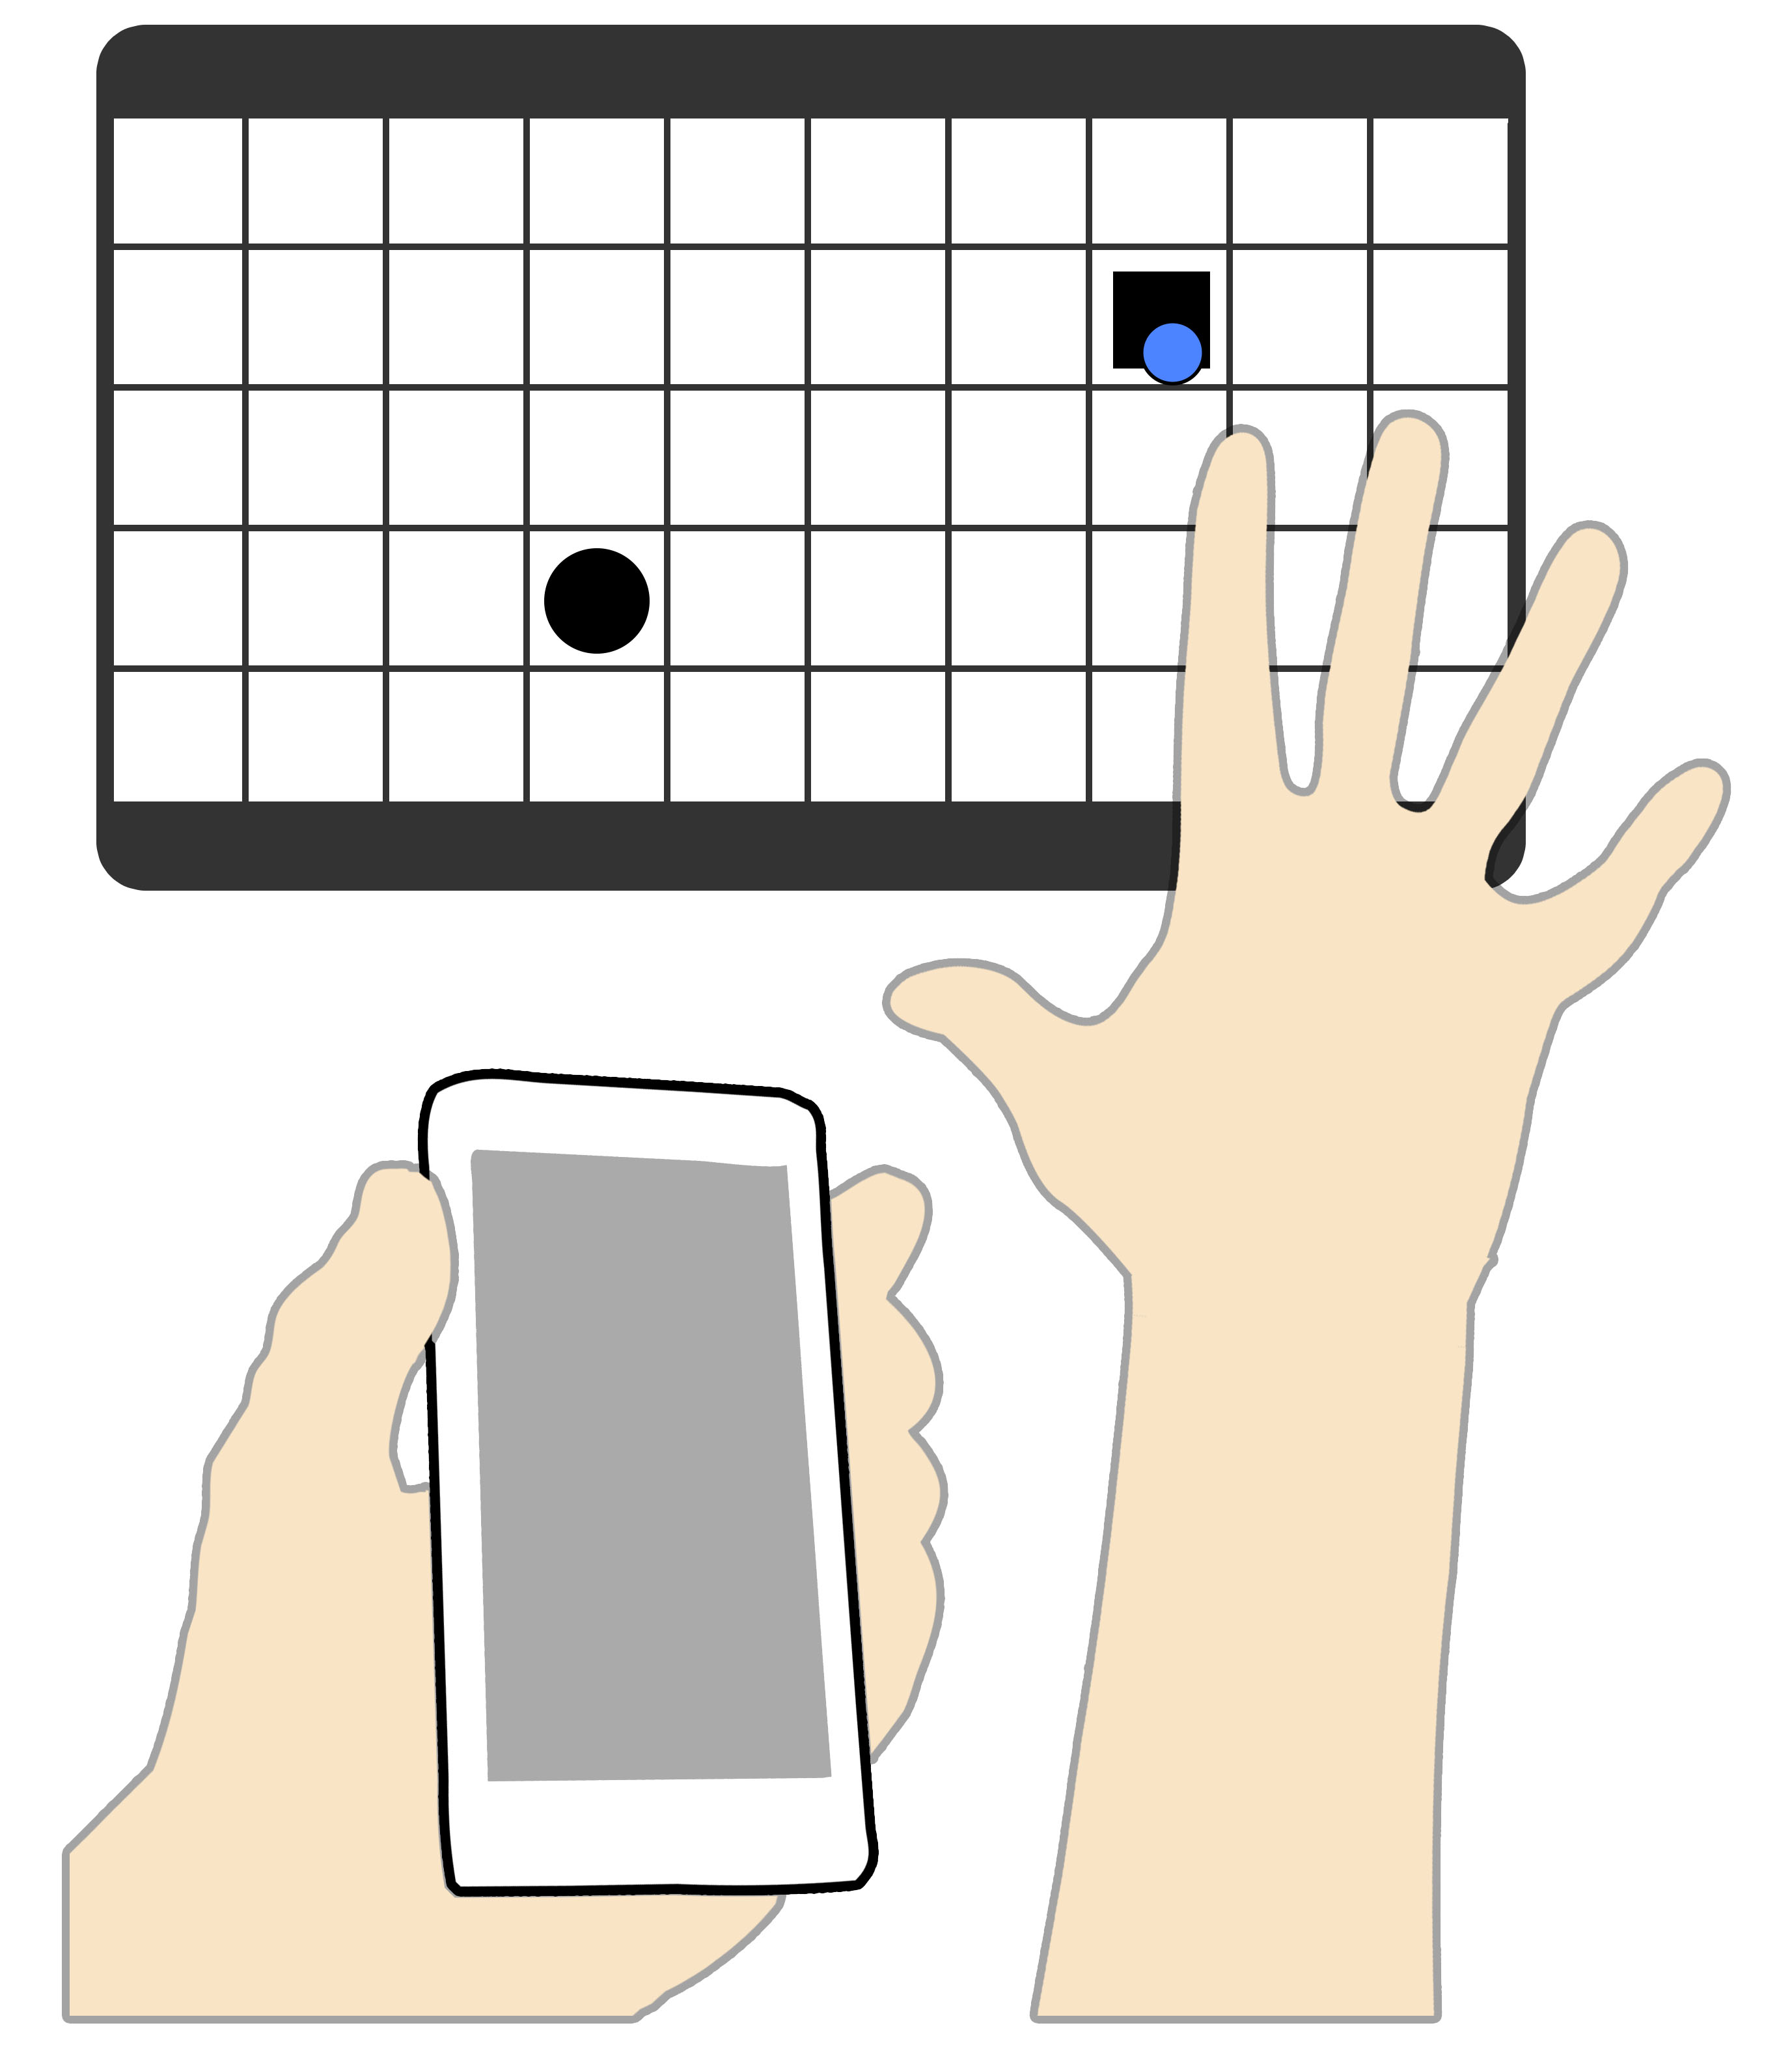
\includegraphics[width = 0.33\columnwidth]{images/techniques/grabPull1.jpg}\label{fig:grabPull1}}
	\subfloat[]{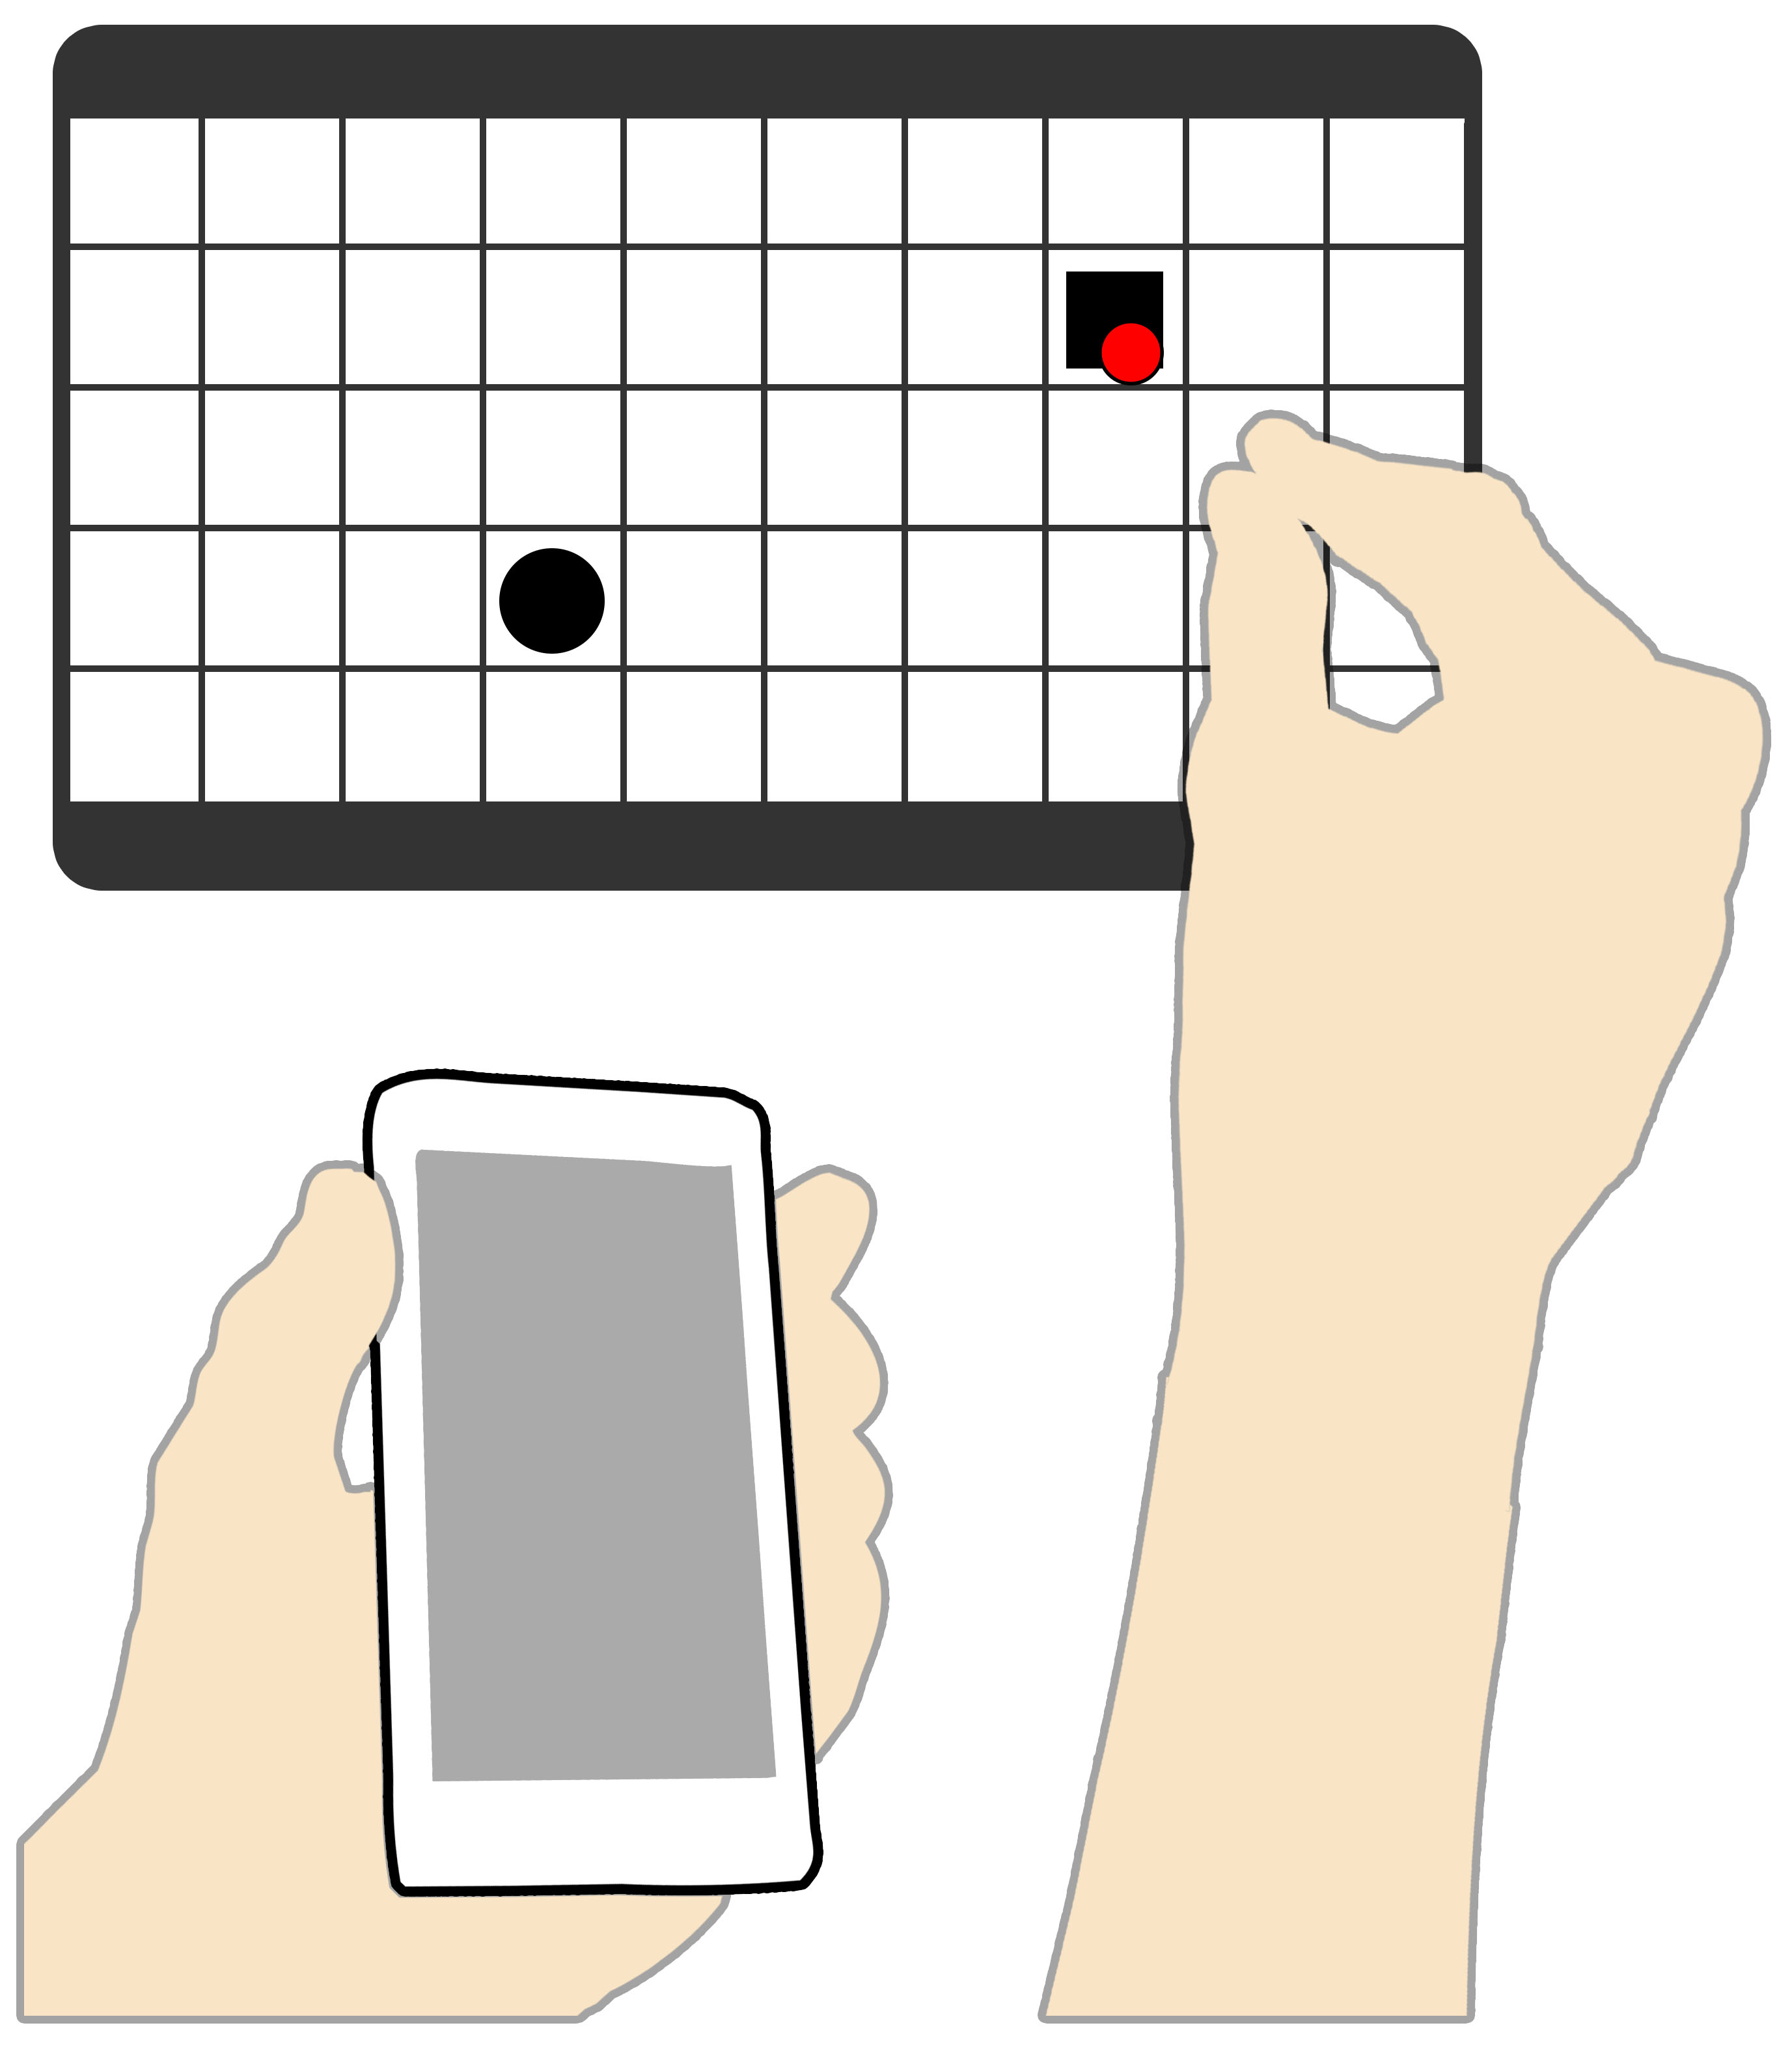
\includegraphics[width = 0.33\columnwidth]{images/techniques/grabPull2.jpg}\label{fig:grabPull2}}
	\subfloat[]{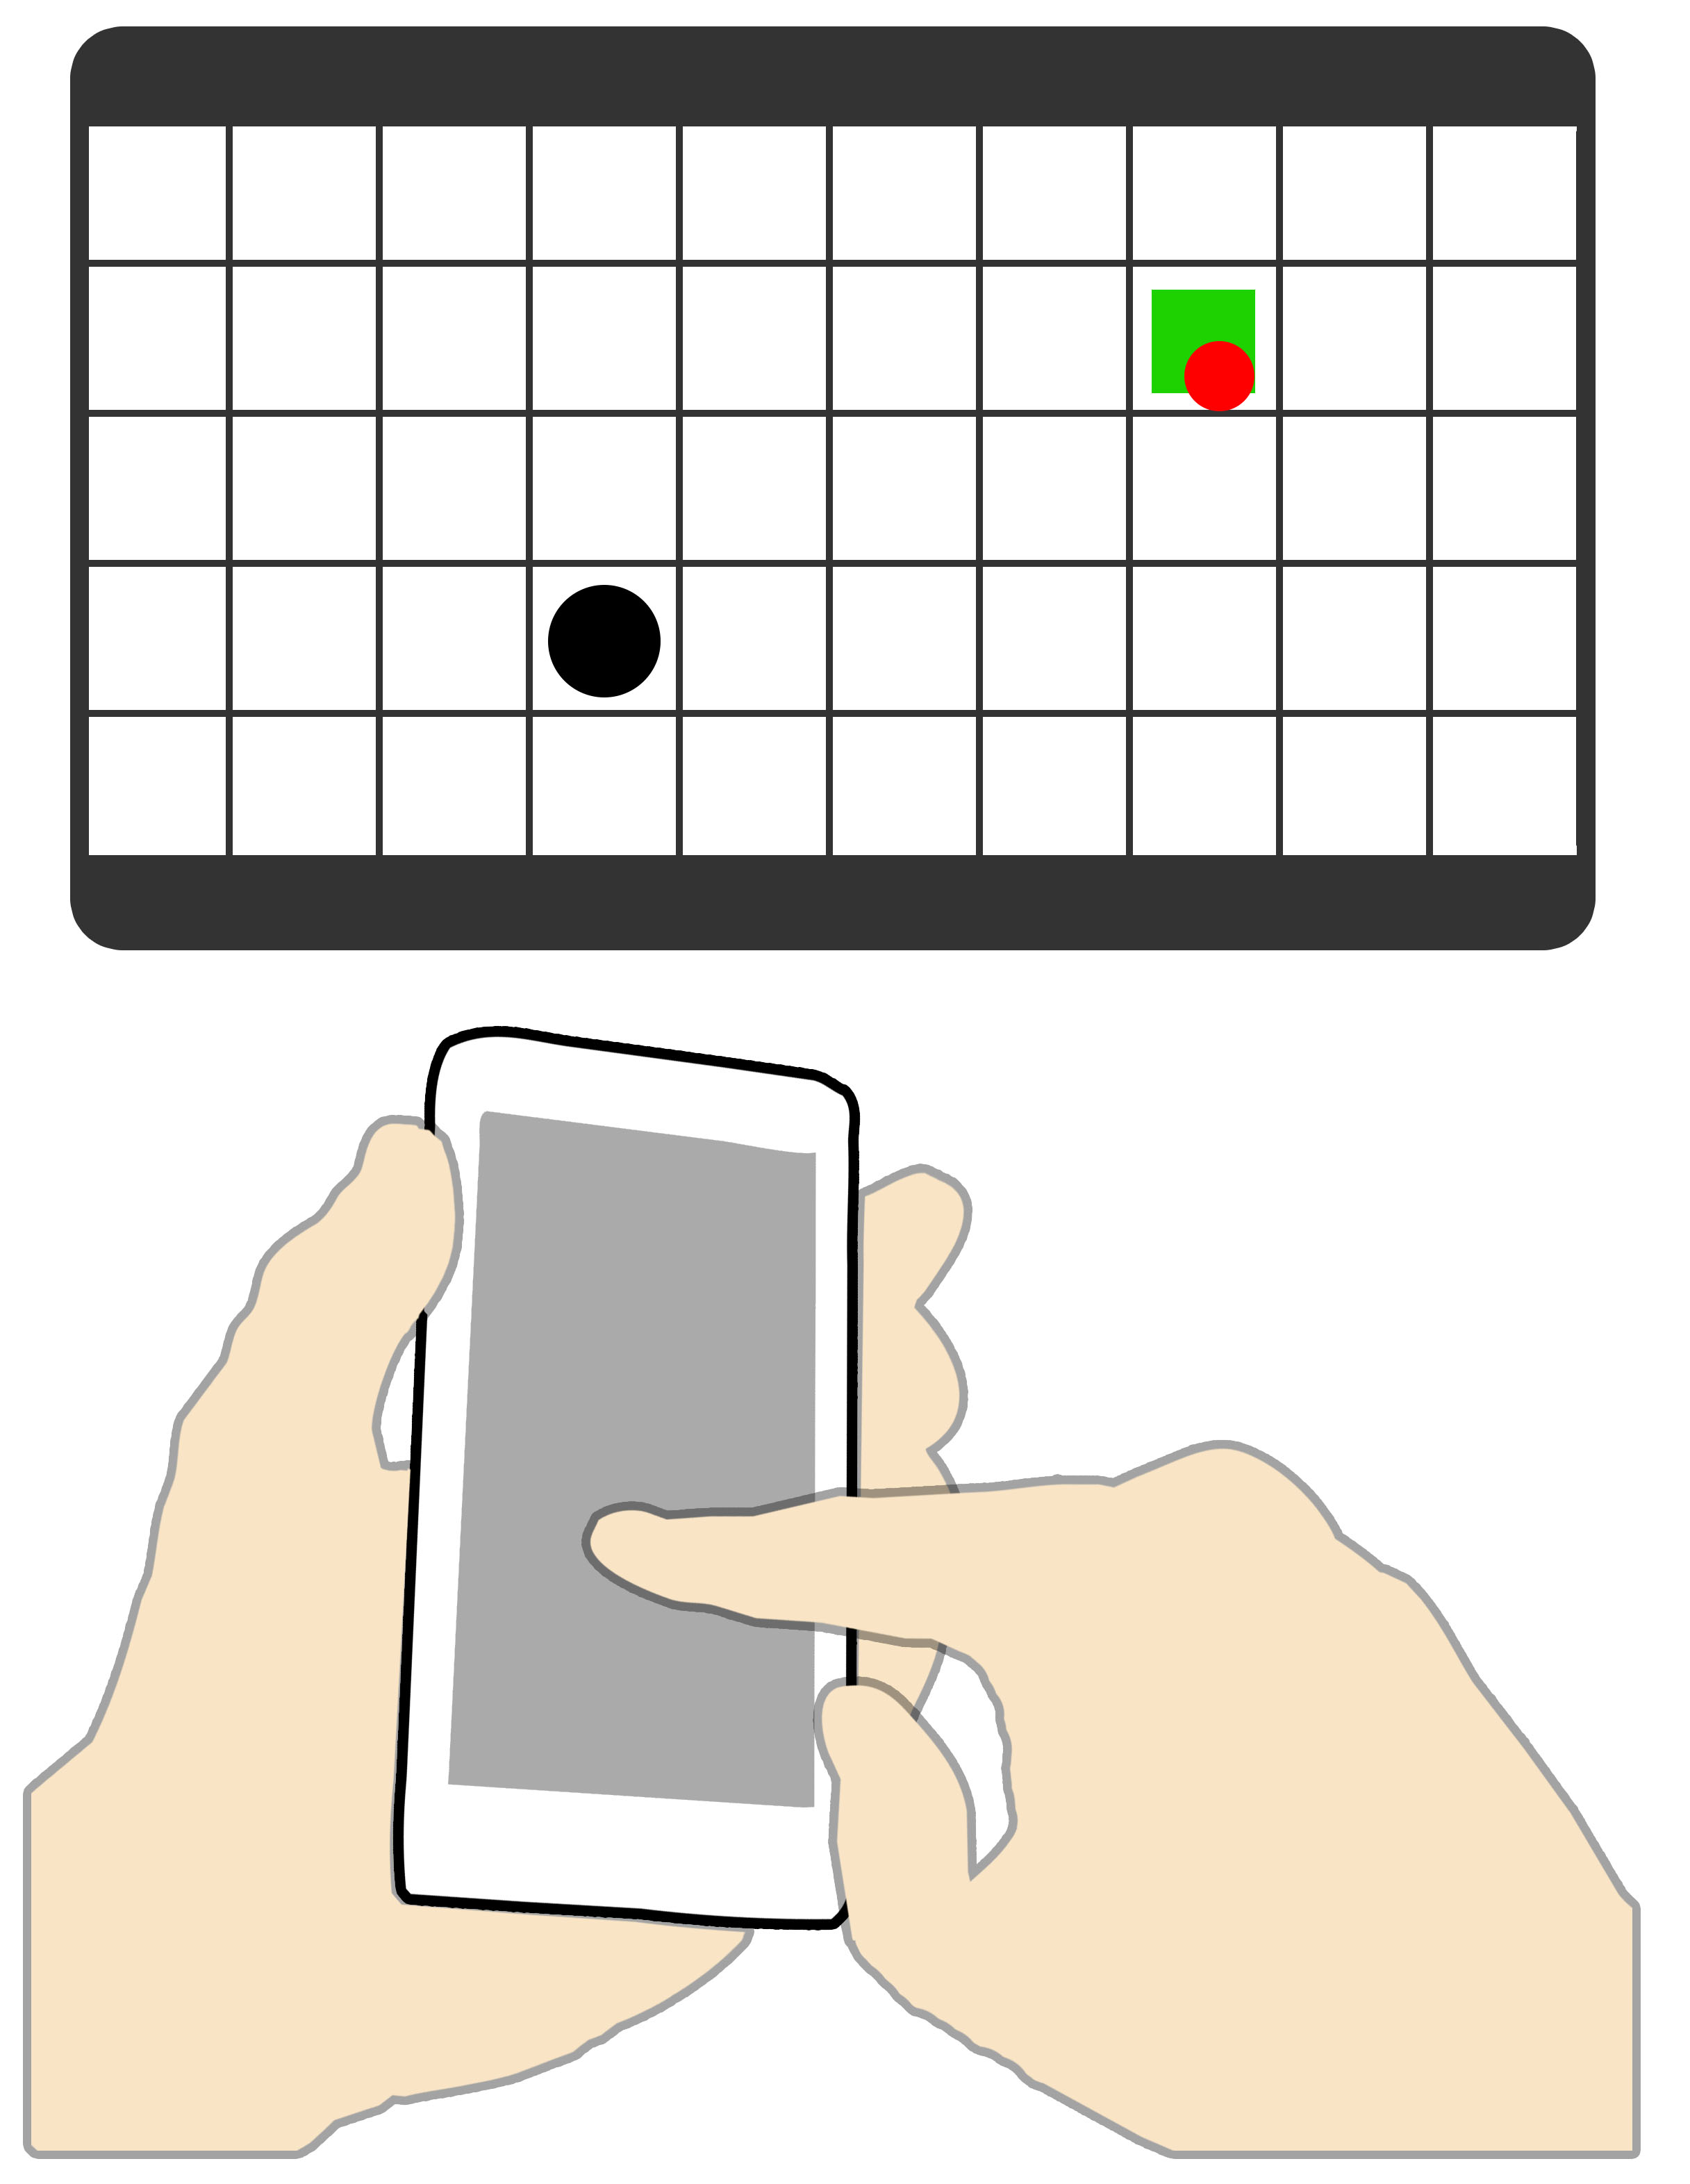
\includegraphics[width = 0.33\columnwidth]{images/techniques/grabPull3.jpg}\label{fig:grabPull3}}
	\caption{\push \grab technique}
	\label{fig:grabTechnique}
\end{figure}

\begin{figure}[H]
	\subfloat[]{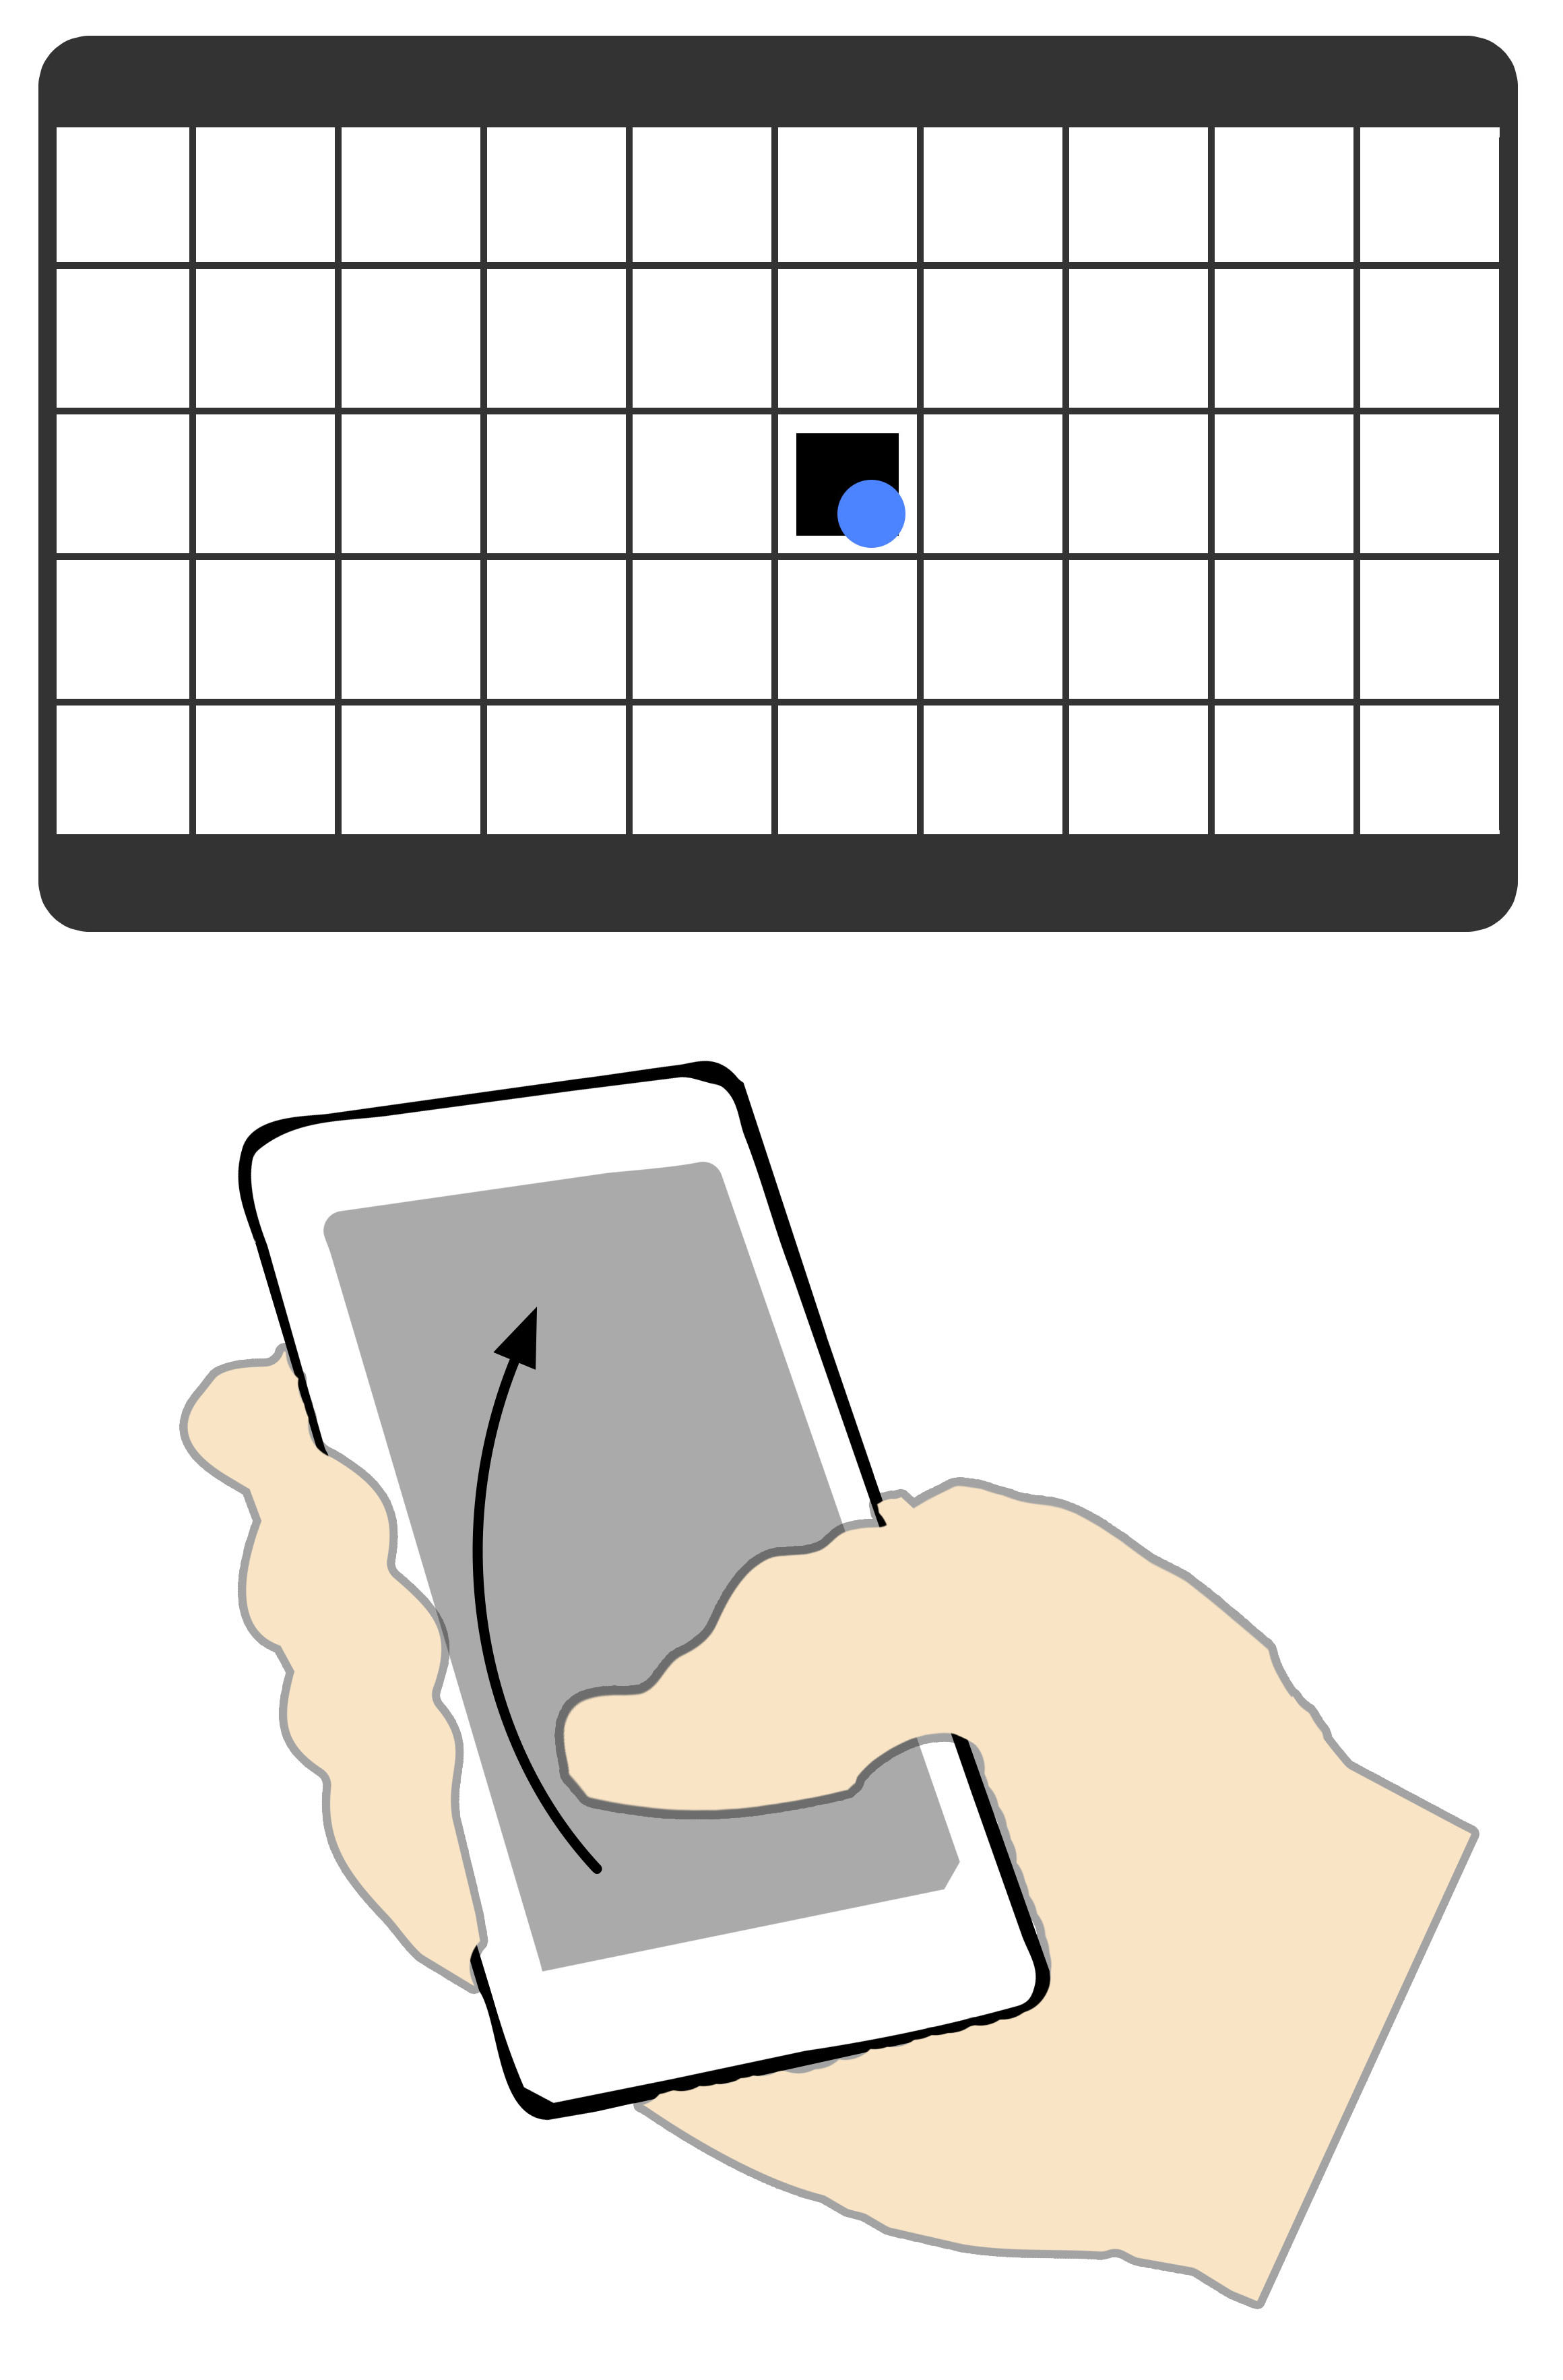
\includegraphics[width = 0.33\columnwidth]{images/techniques/swipePush1.jpg}\label{fig:swipePush1}}
	\subfloat[]{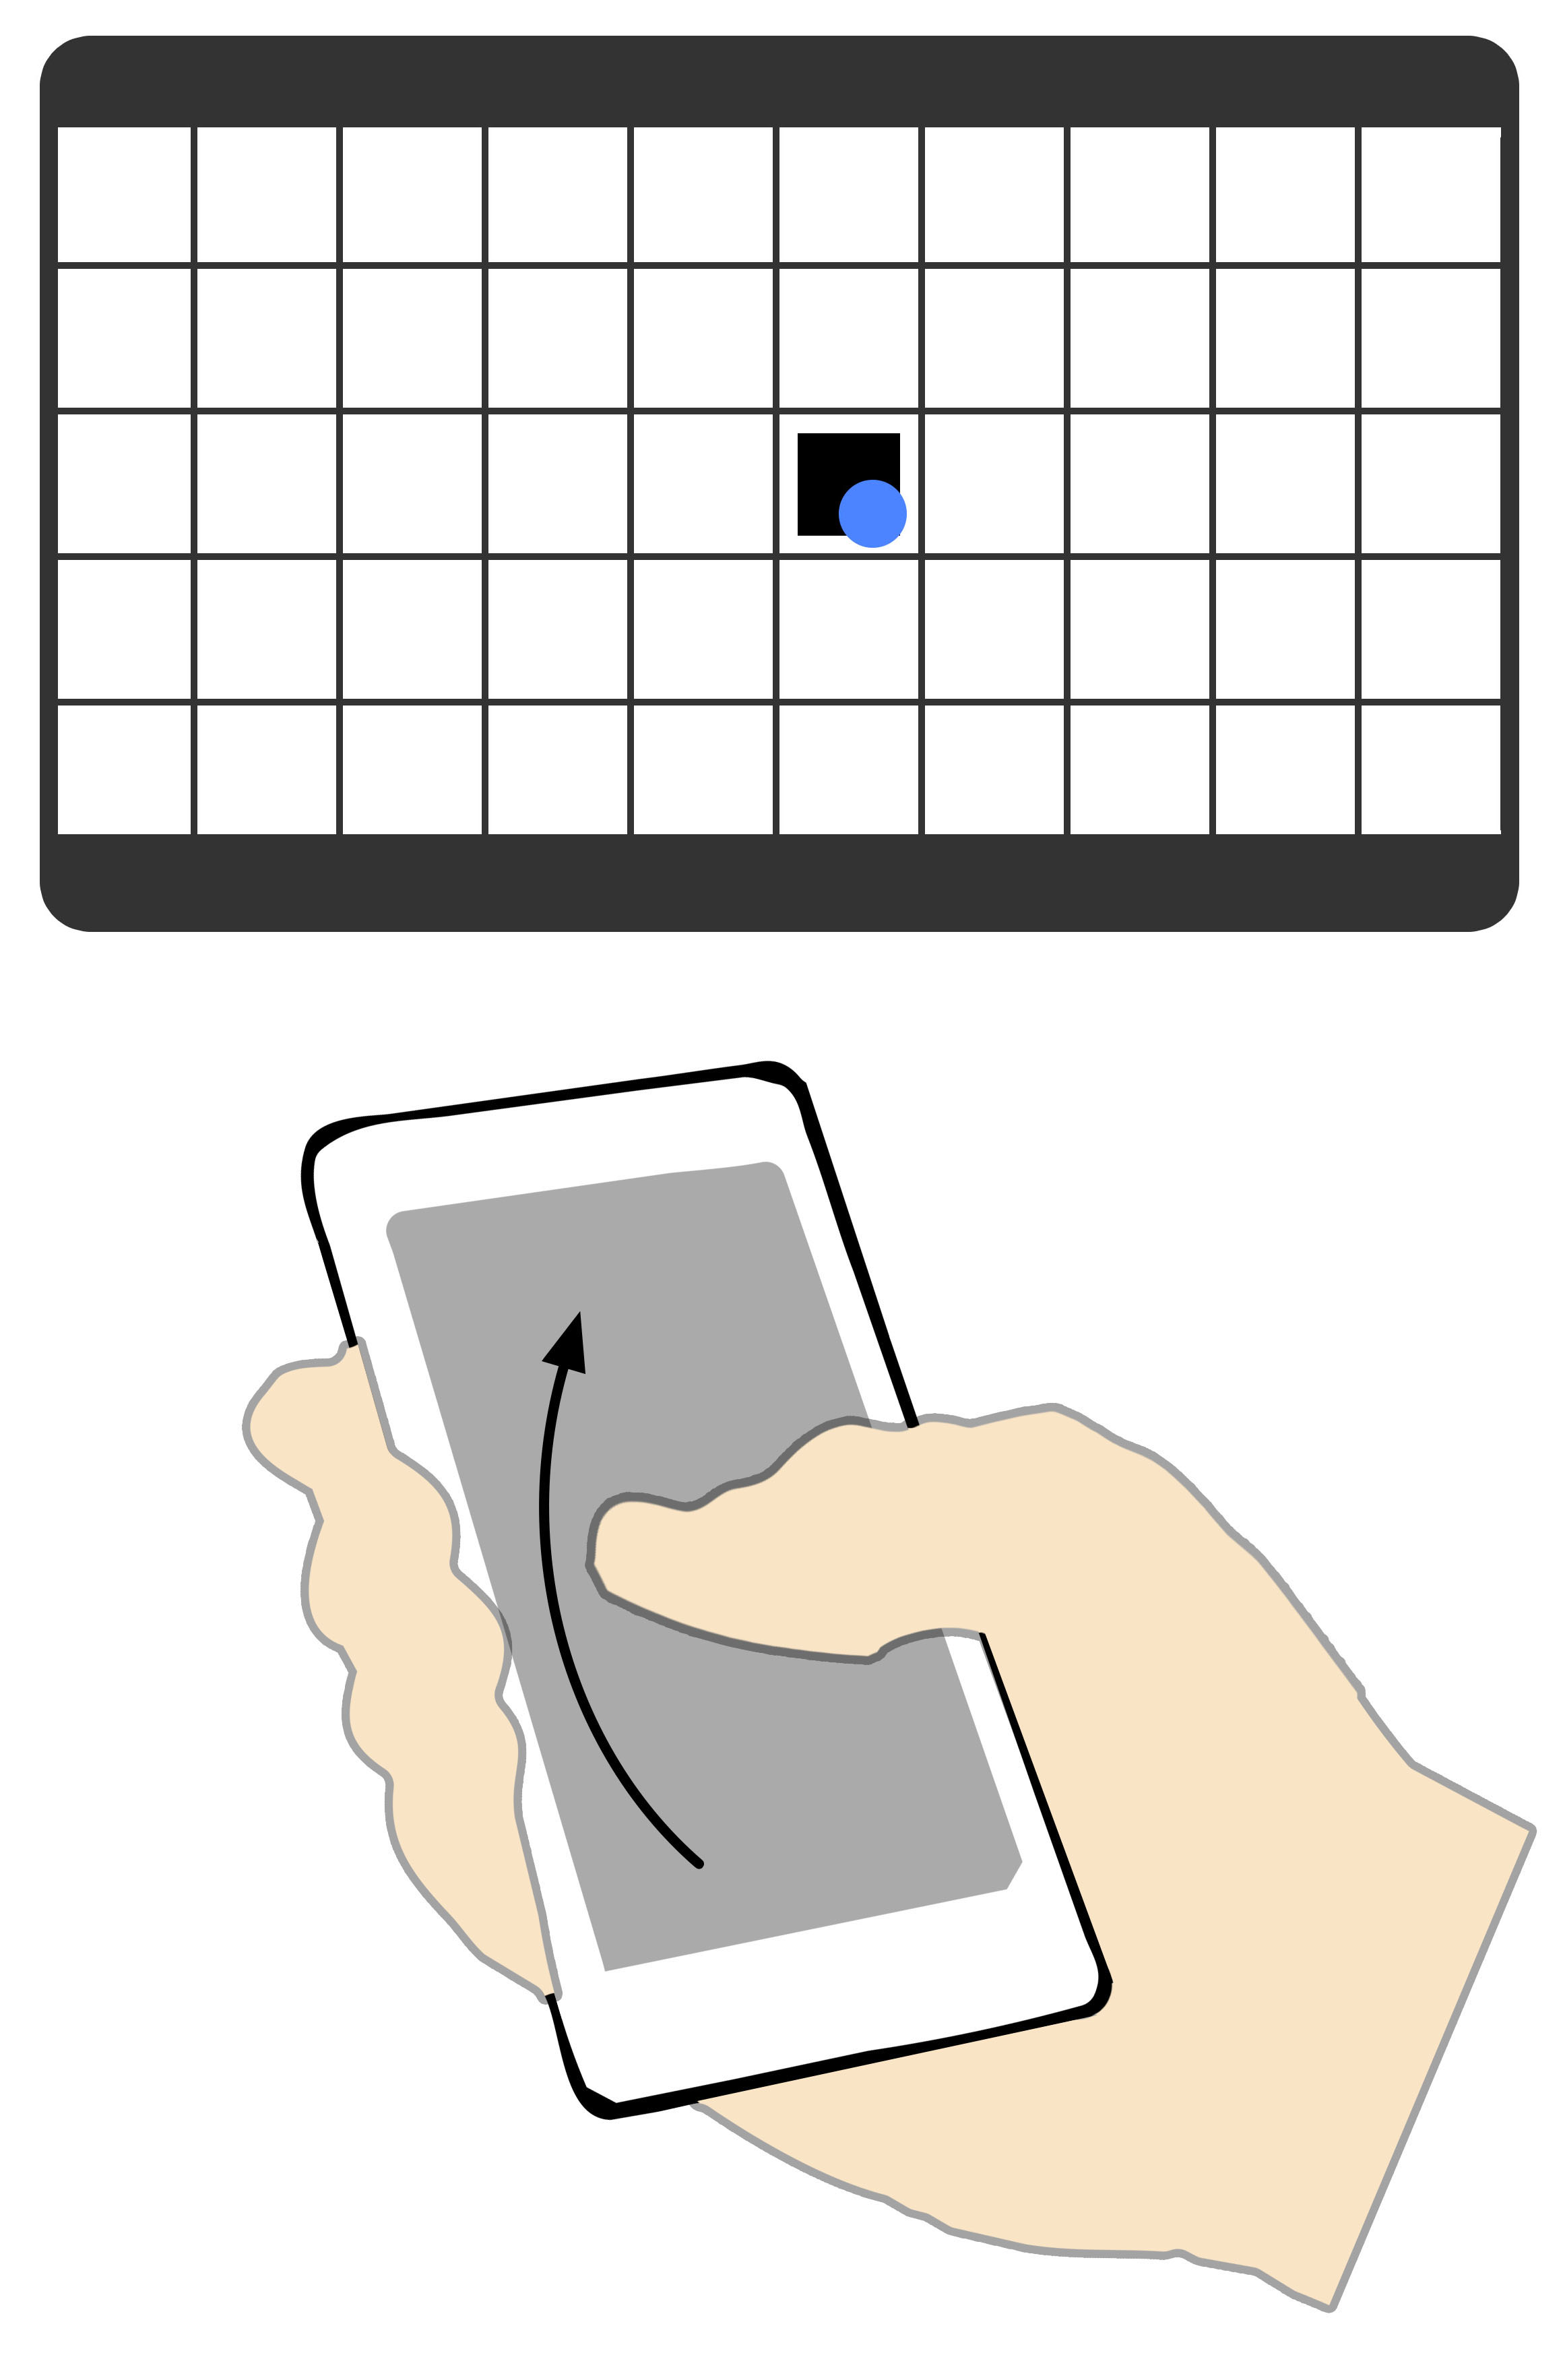
\includegraphics[width = 0.33\columnwidth]{images/techniques/swipePush2.jpg}\label{fig:swipePush2}}
	\subfloat[]{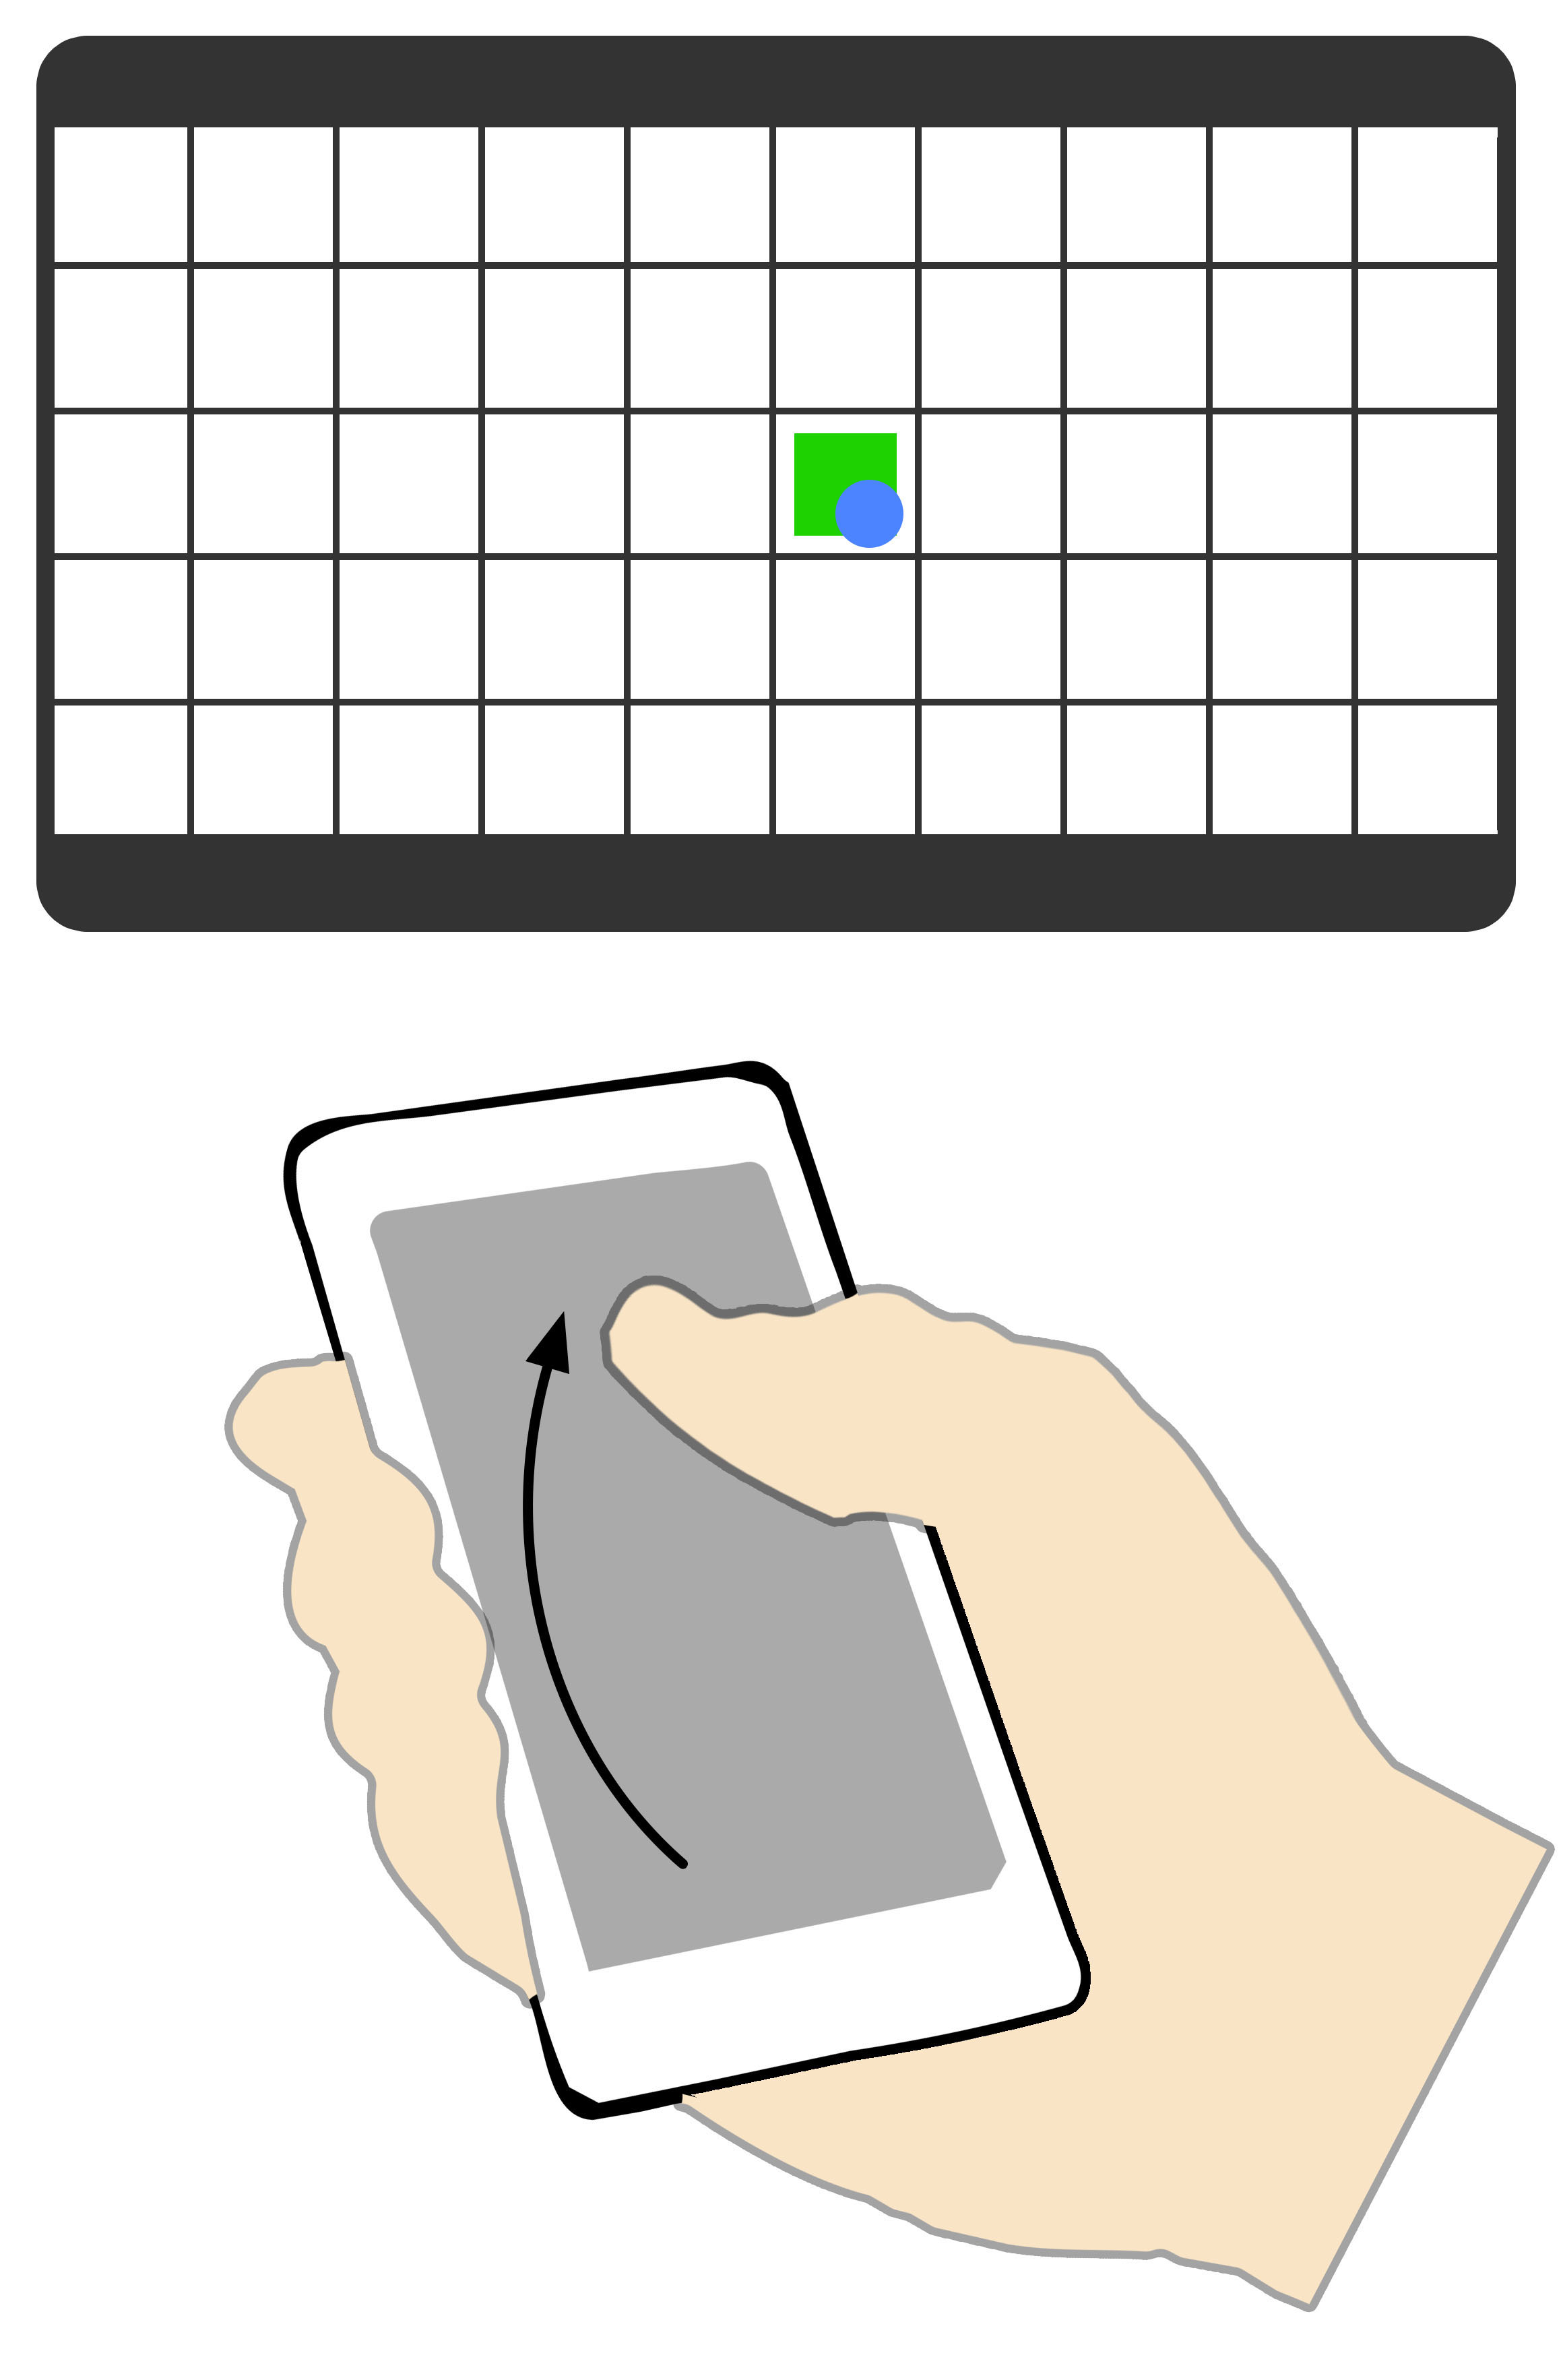
\includegraphics[width = 0.33\columnwidth]{images/techniques/swipePush3.jpg}\label{fig:swipePush3}}
	\caption{\push \grab technique}
	\label{fig:grabTechnique}
\end{figure}

\begin{figure}[H]
	\subfloat[]{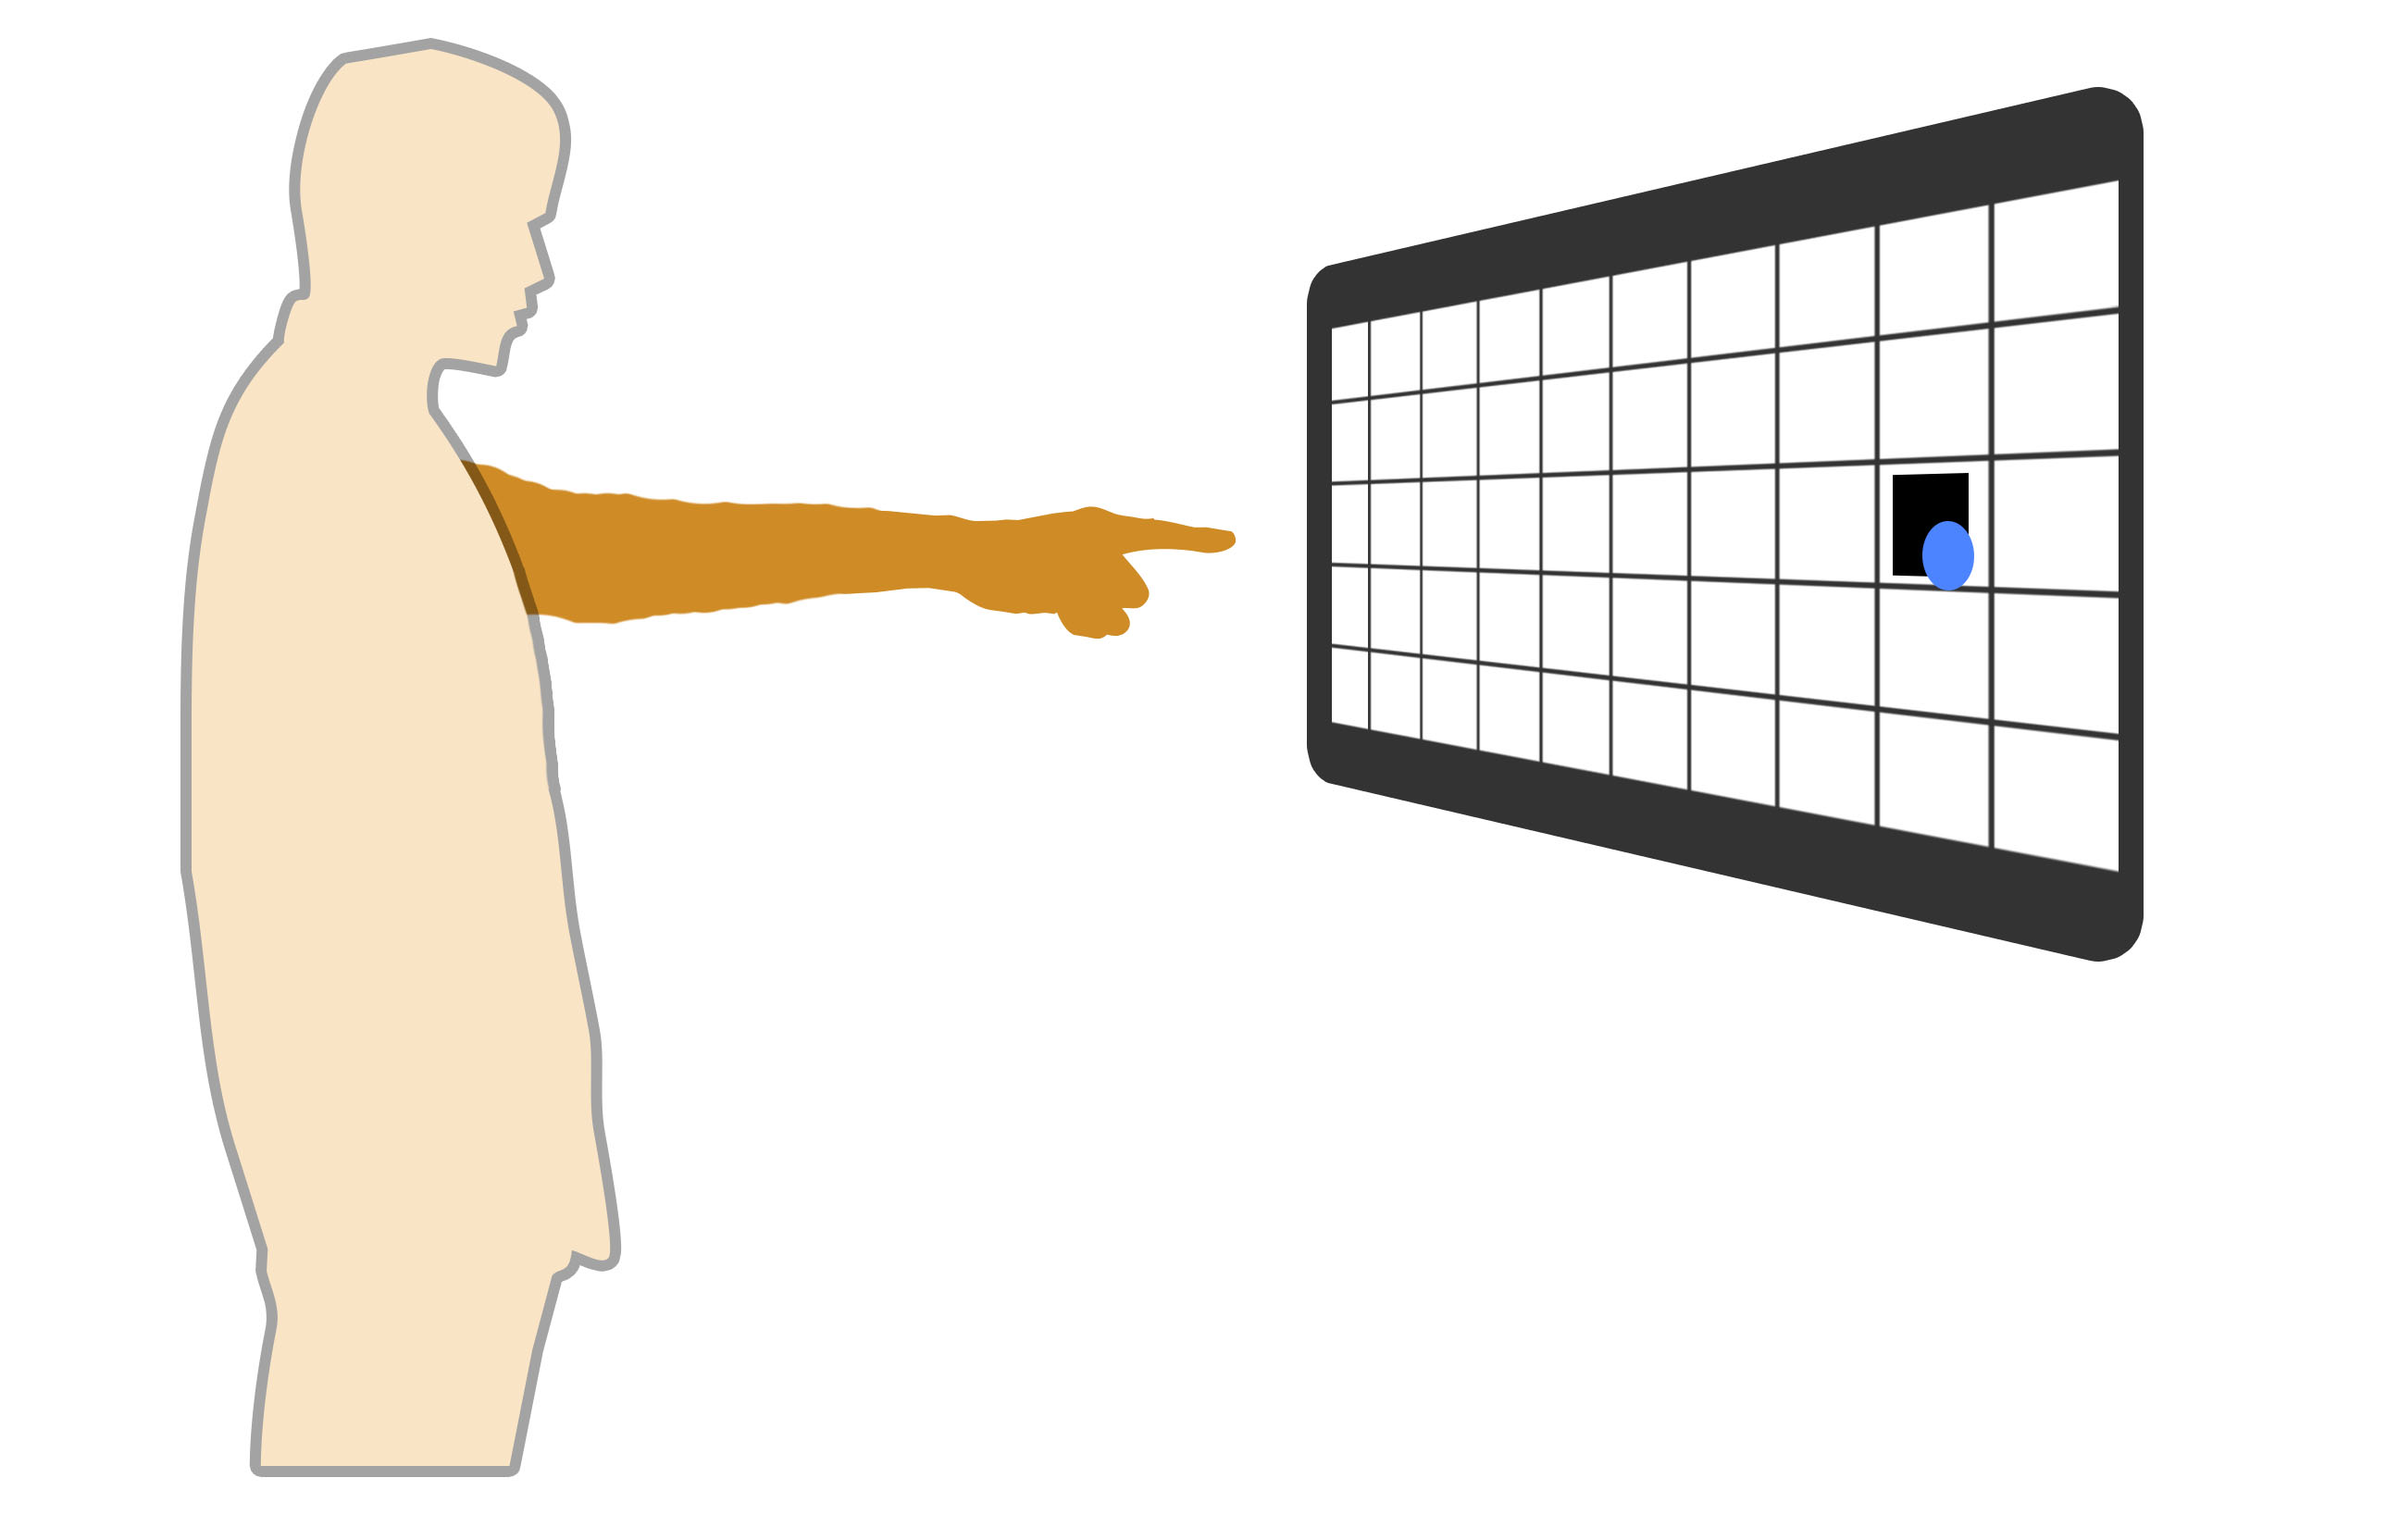
\includegraphics[width = 0.33\columnwidth]{images/techniques/throwPush1.jpg}\label{fig:throwPush1}}
	\subfloat[]{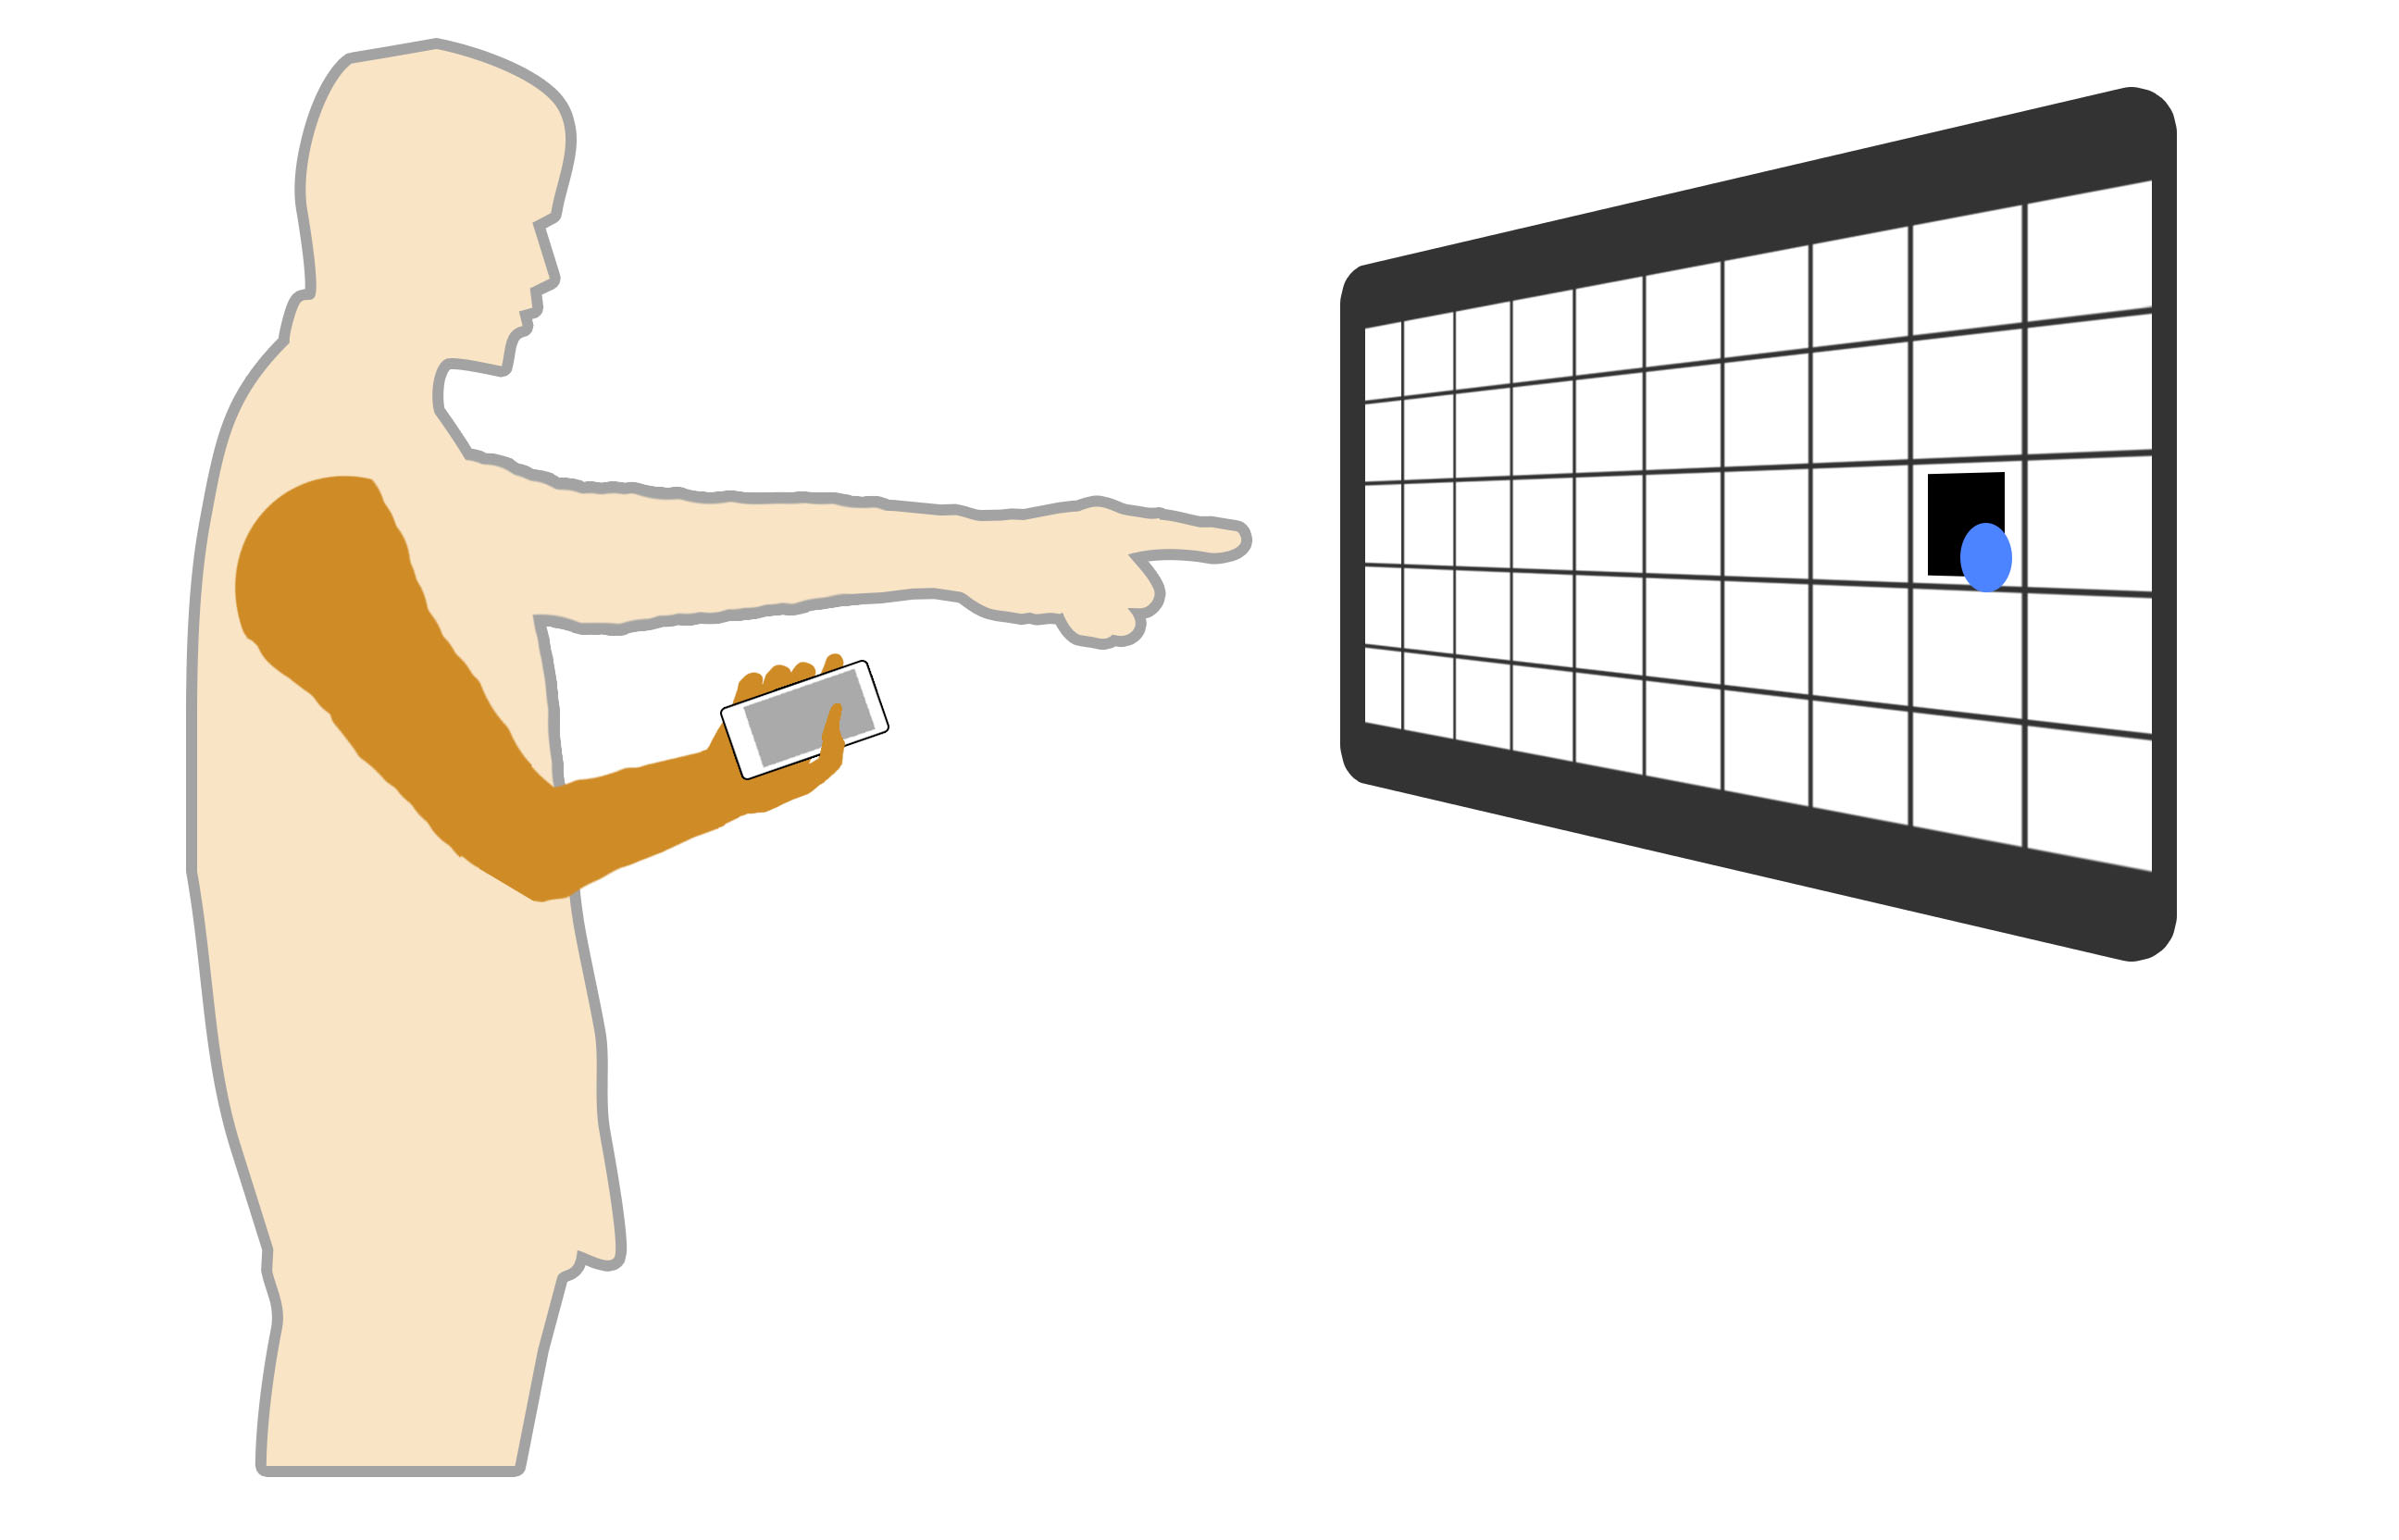
\includegraphics[width = 0.33\columnwidth]{images/techniques/throwPush2.jpg}\label{fig:throwPush2}}
	\subfloat[]{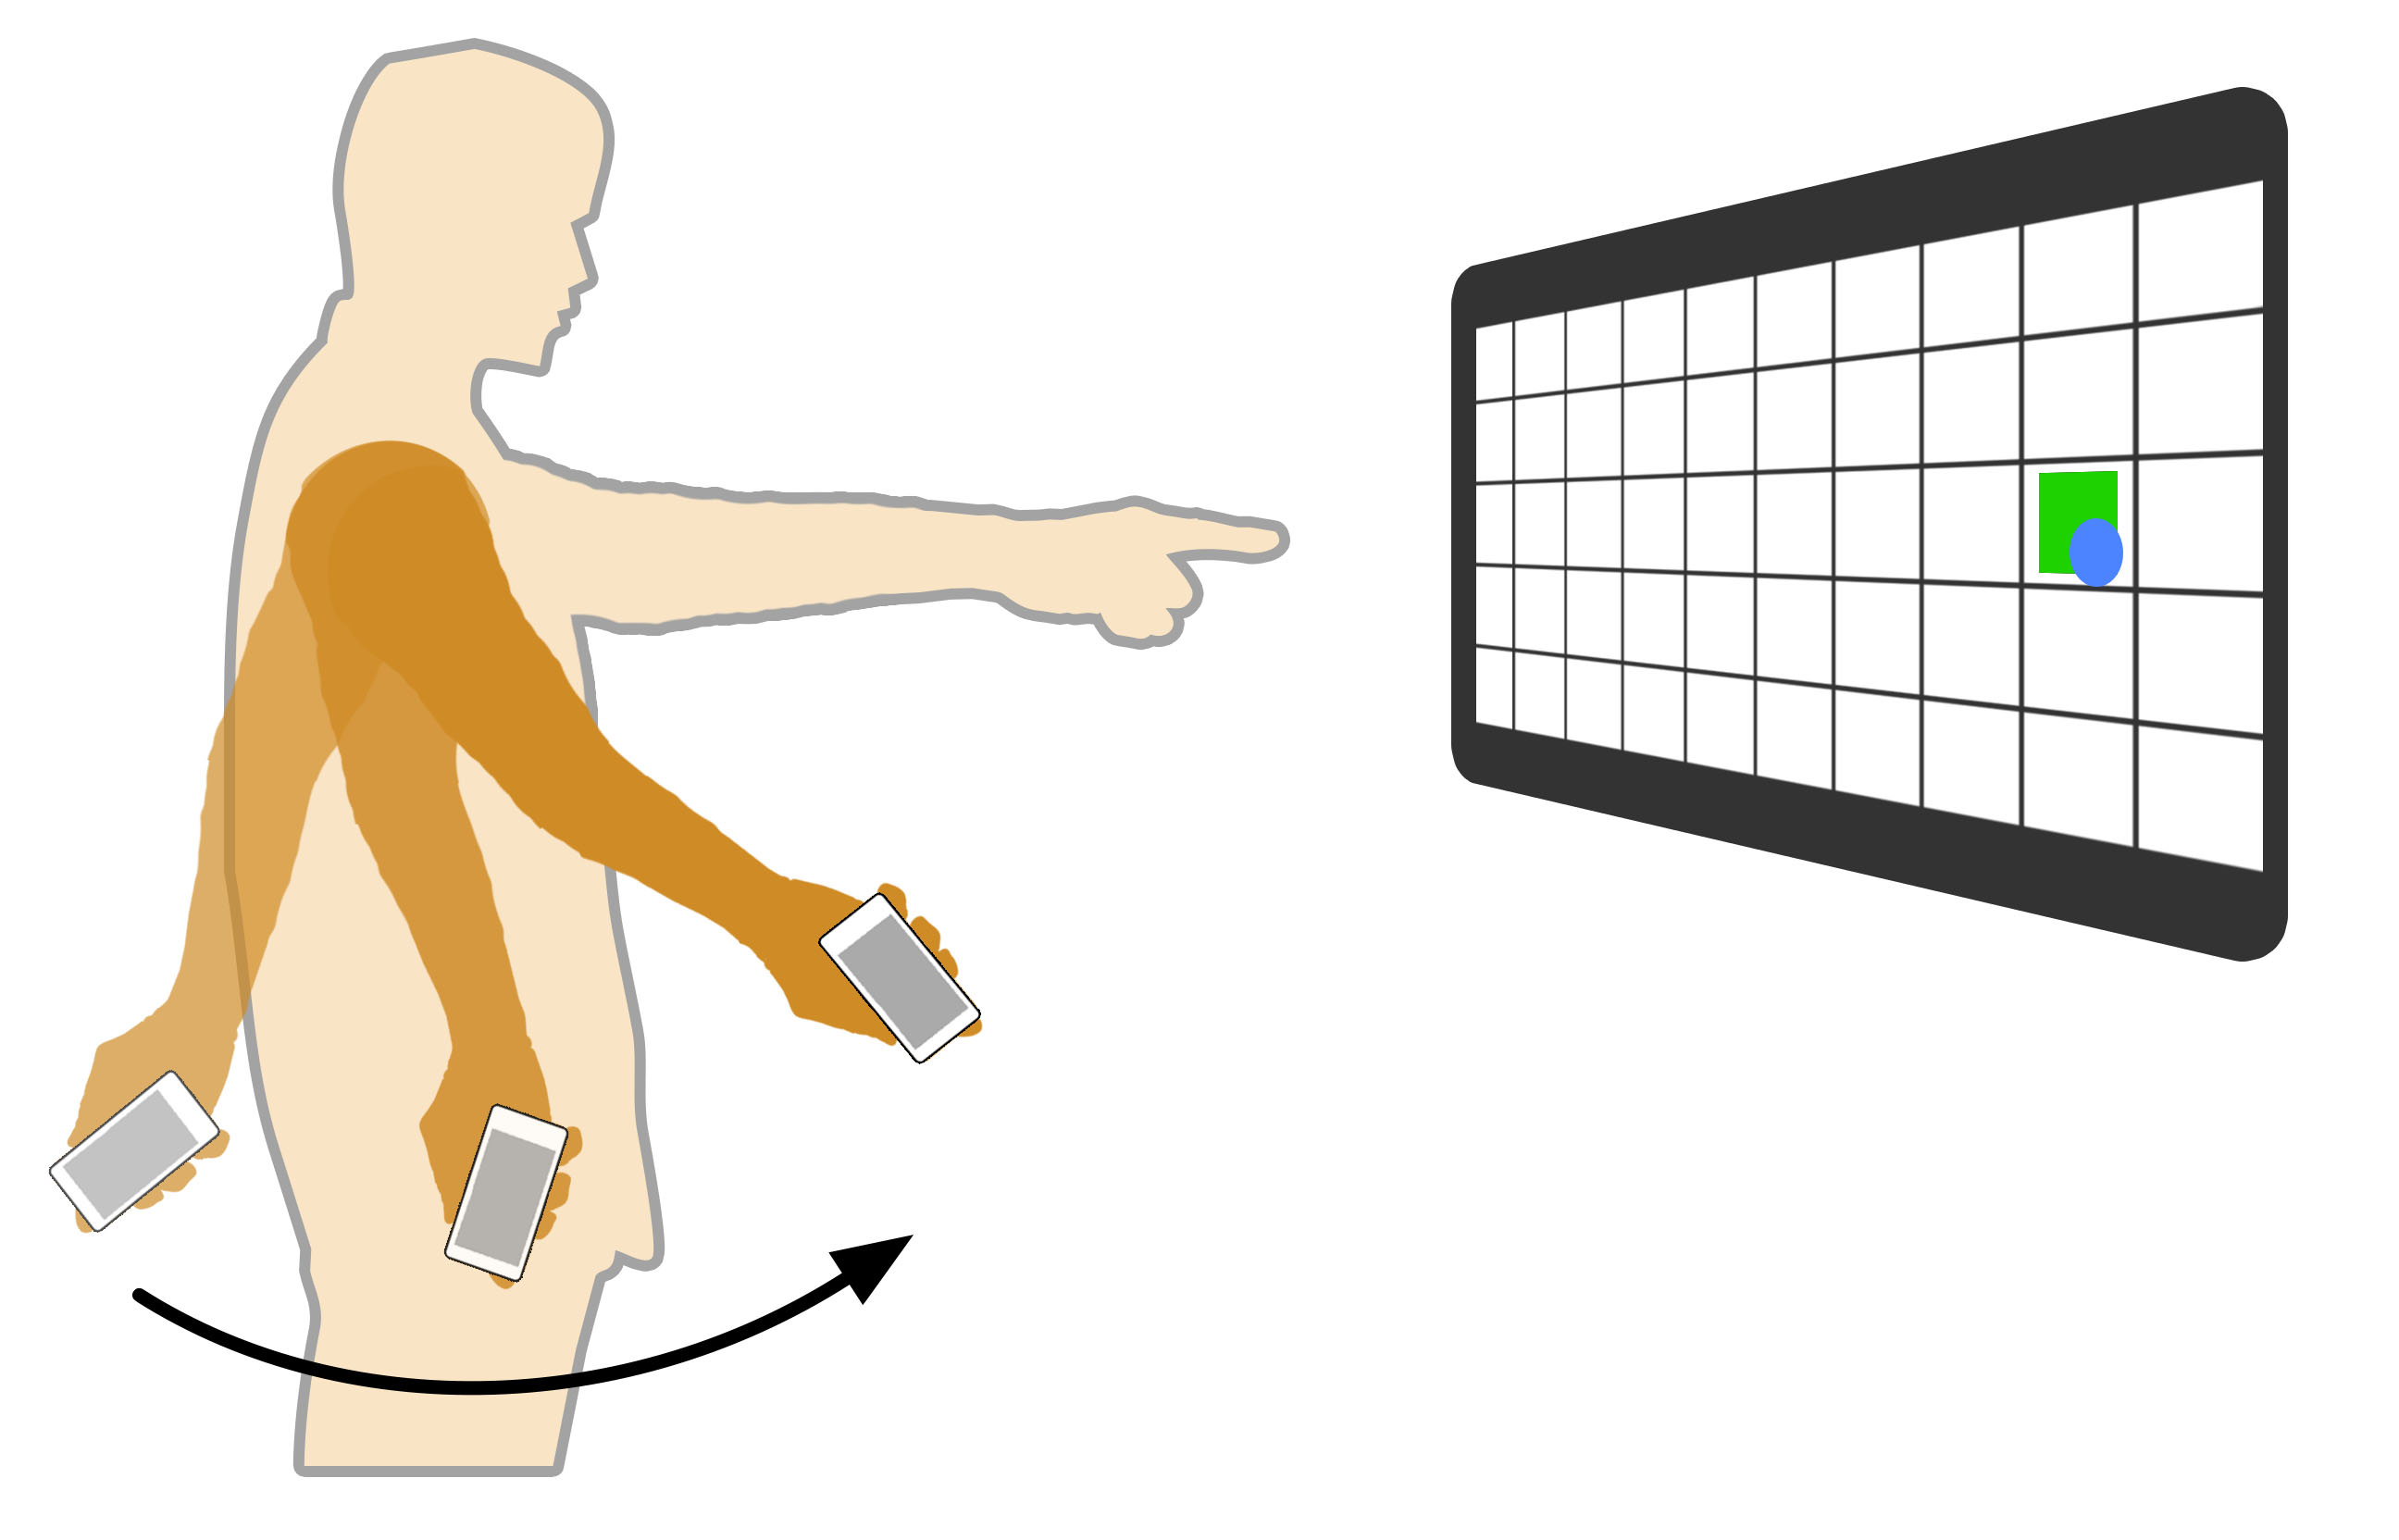
\includegraphics[width = 0.33\columnwidth]{images/techniques/throwPush3.jpg}\label{fig:throwPush3}}
	\caption{\push \grab technique}
	\label{fig:grabTechnique}
\end{figure}

\begin{figure}[H]
	\subfloat[]{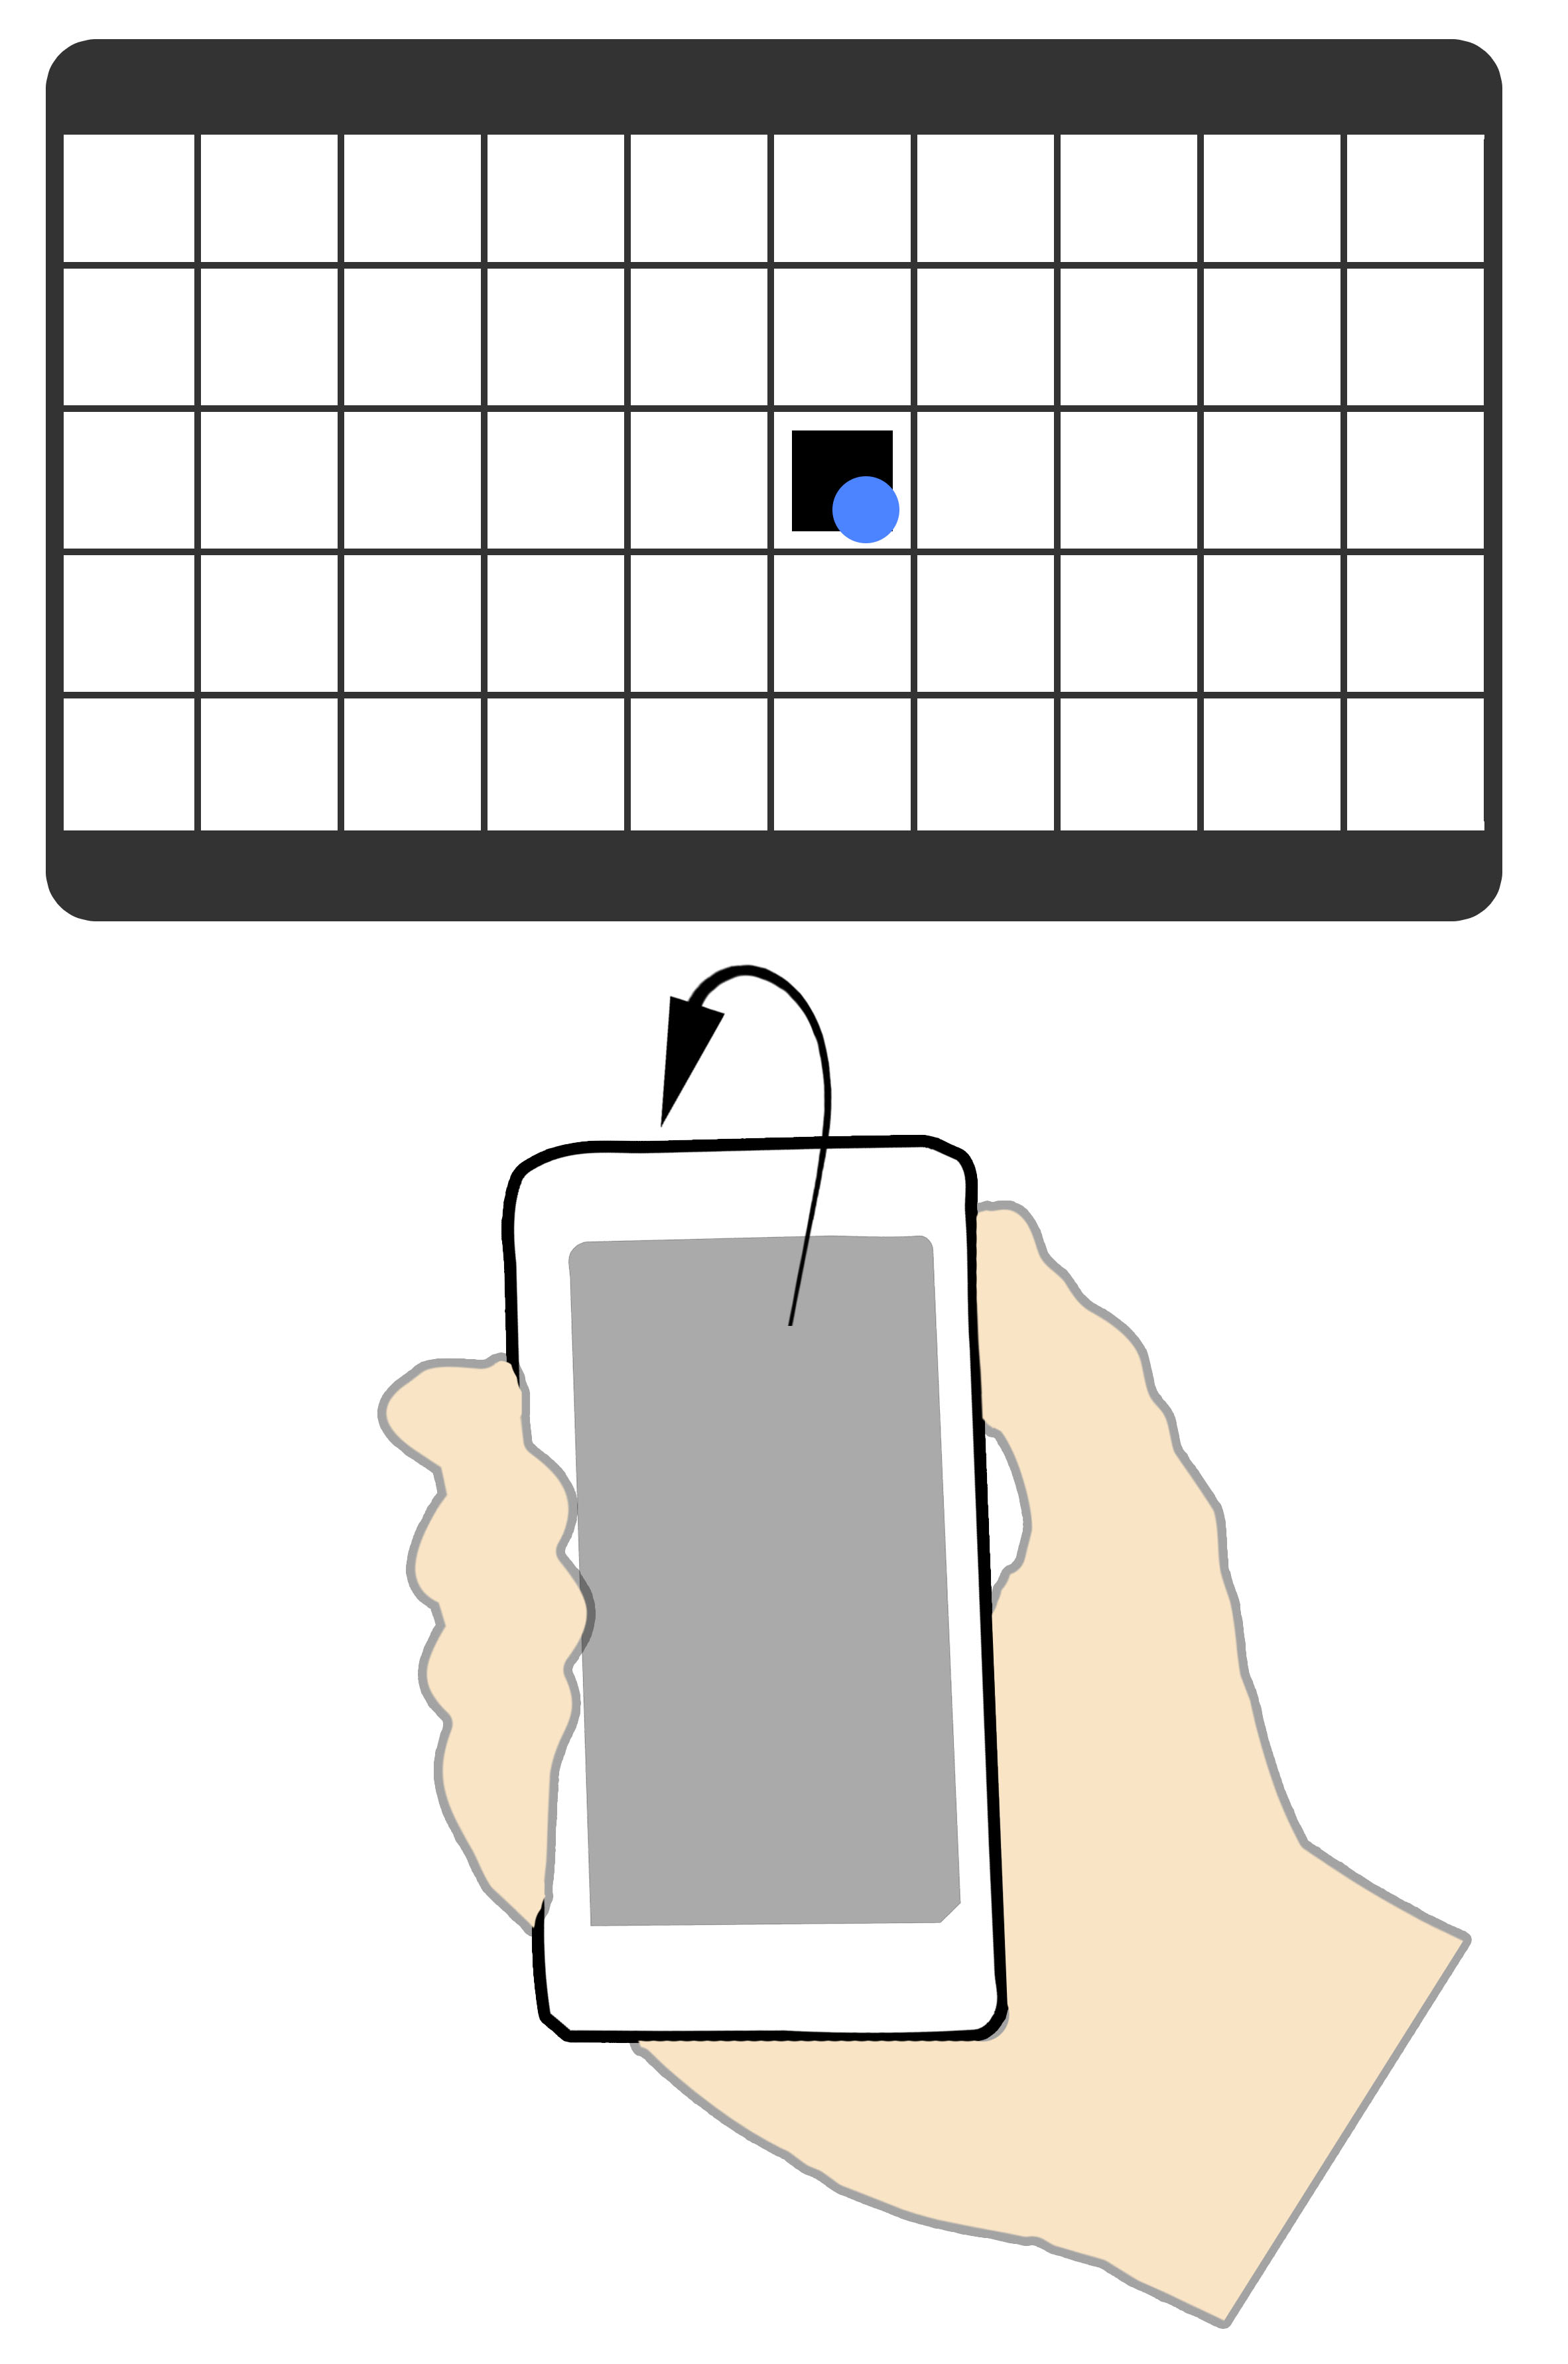
\includegraphics[width = 0.33\columnwidth]{images/techniques/tiltPush1.jpg}\label{fig:tiltPush1}}
	\subfloat[]{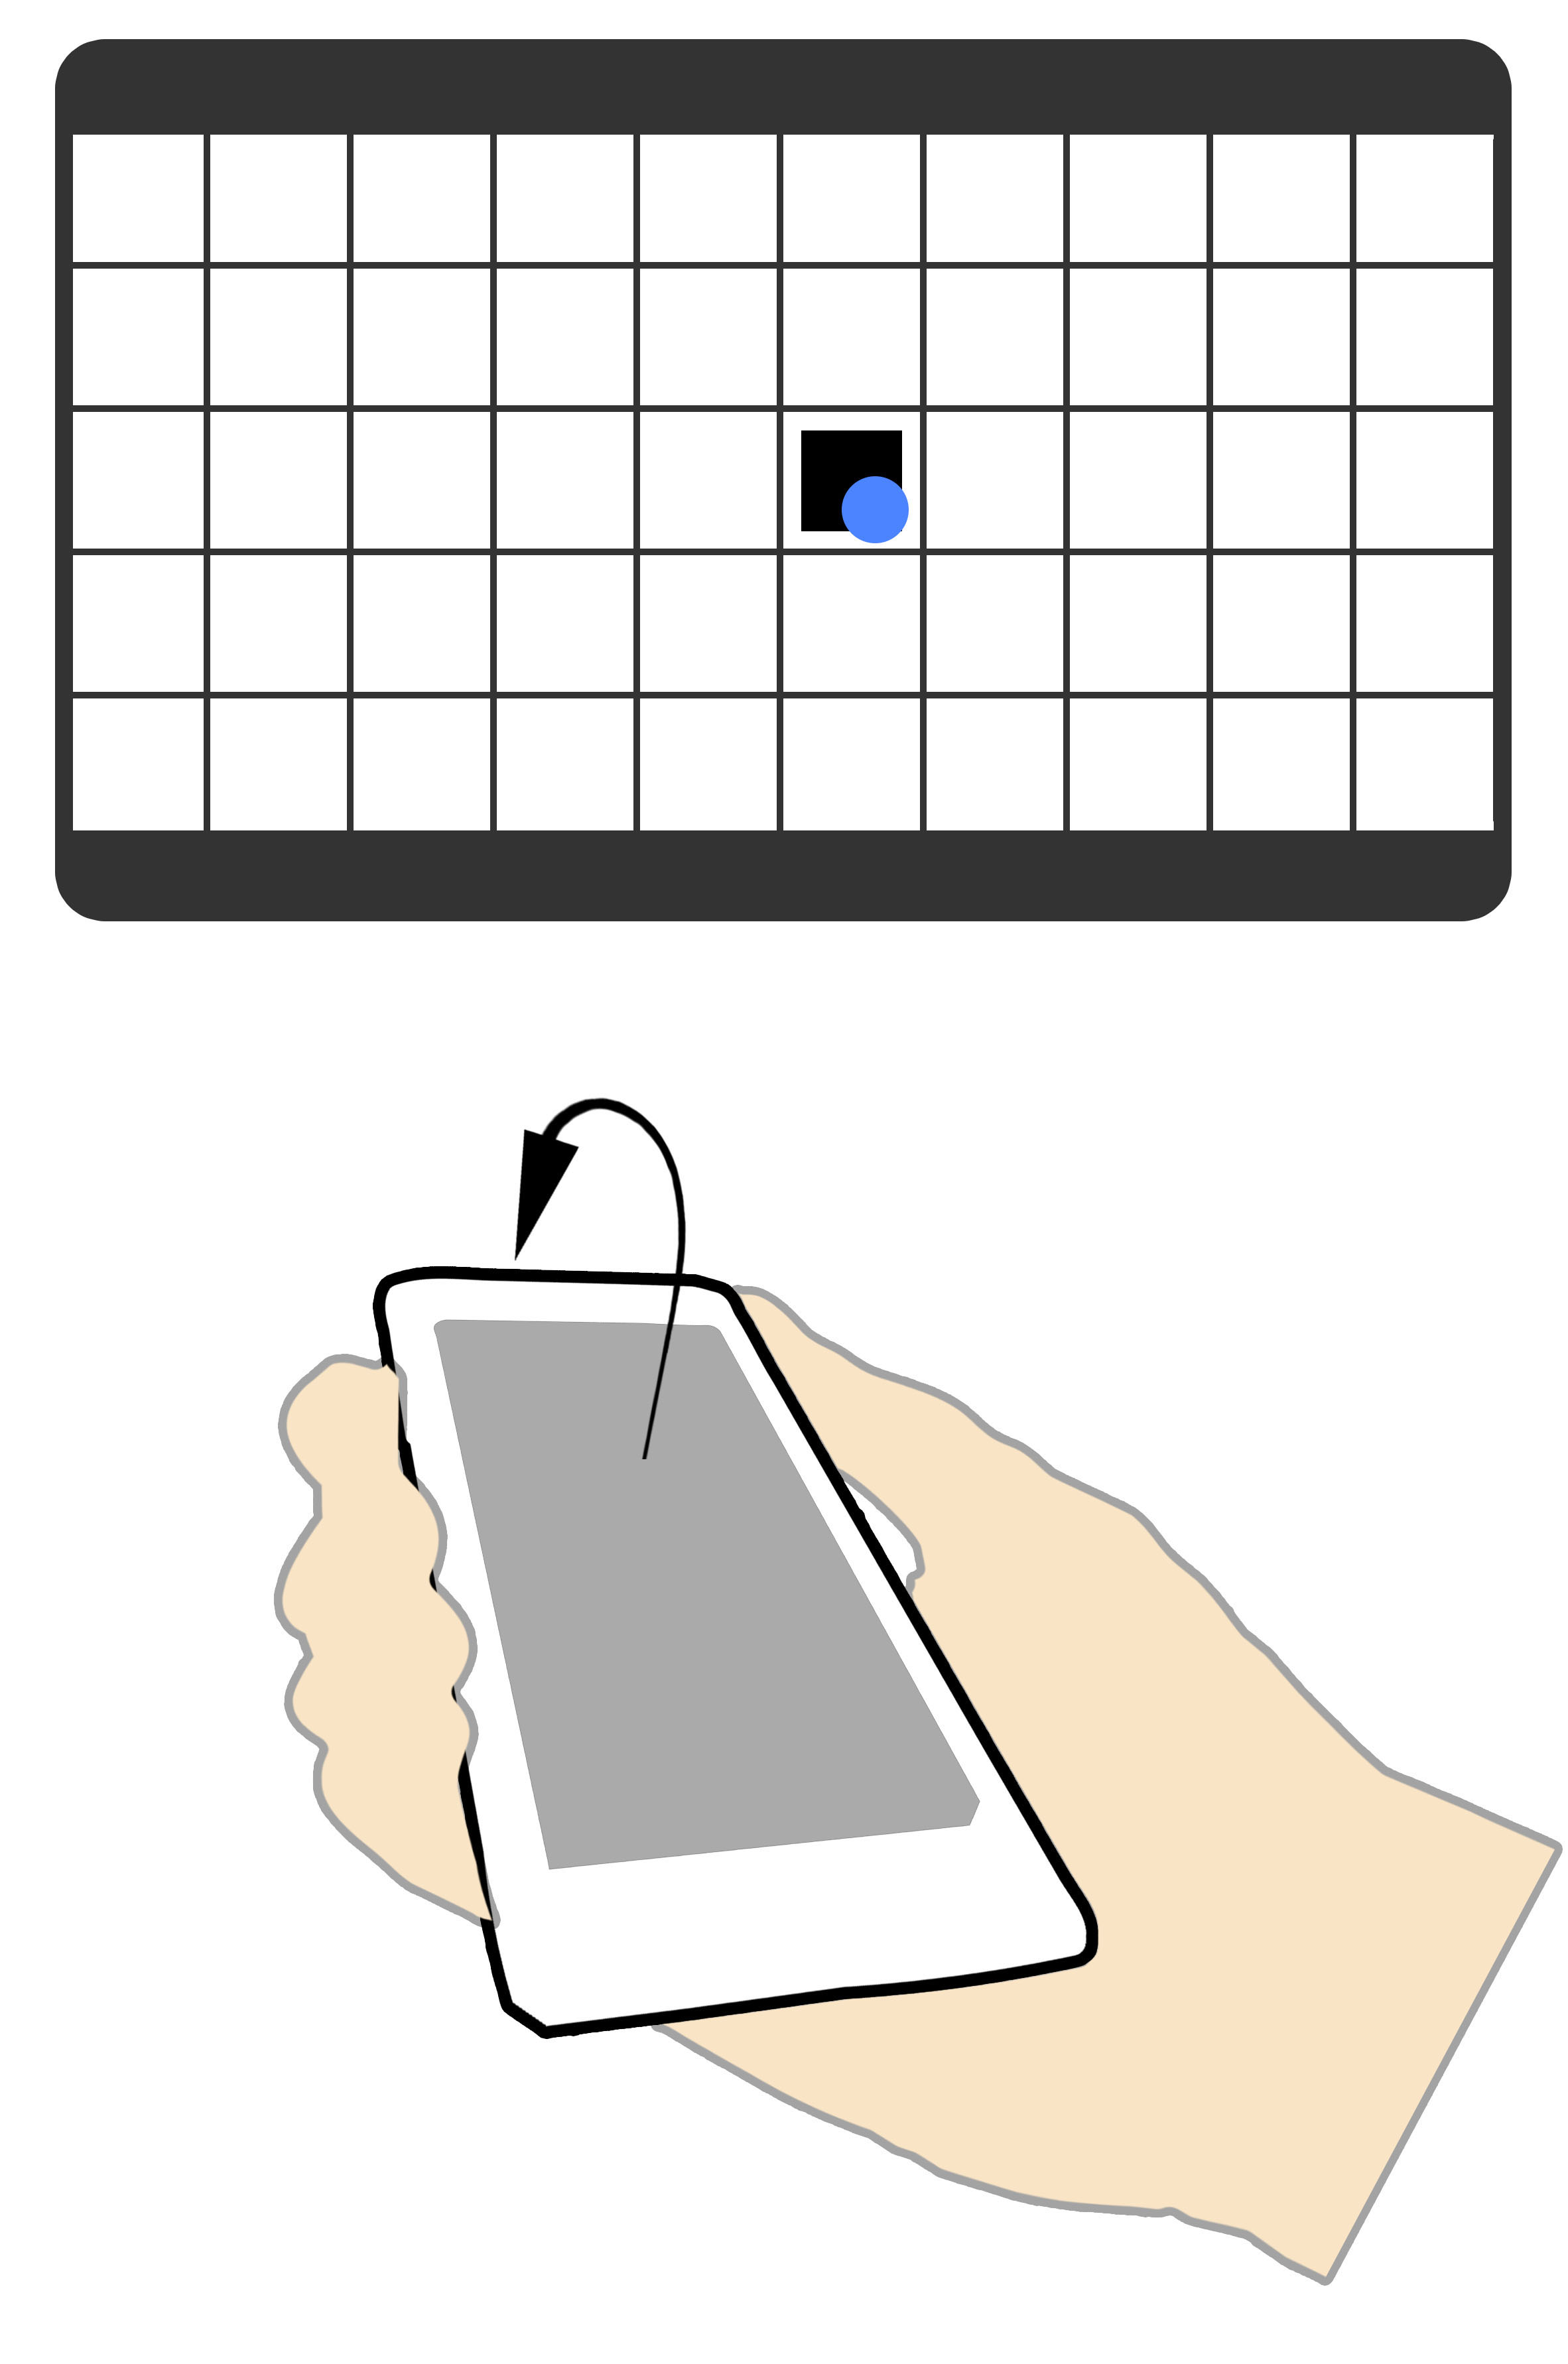
\includegraphics[width = 0.33\columnwidth]{images/techniques/tiltPush2.jpg}\label{fig:tiltPush2}}
	\subfloat[]{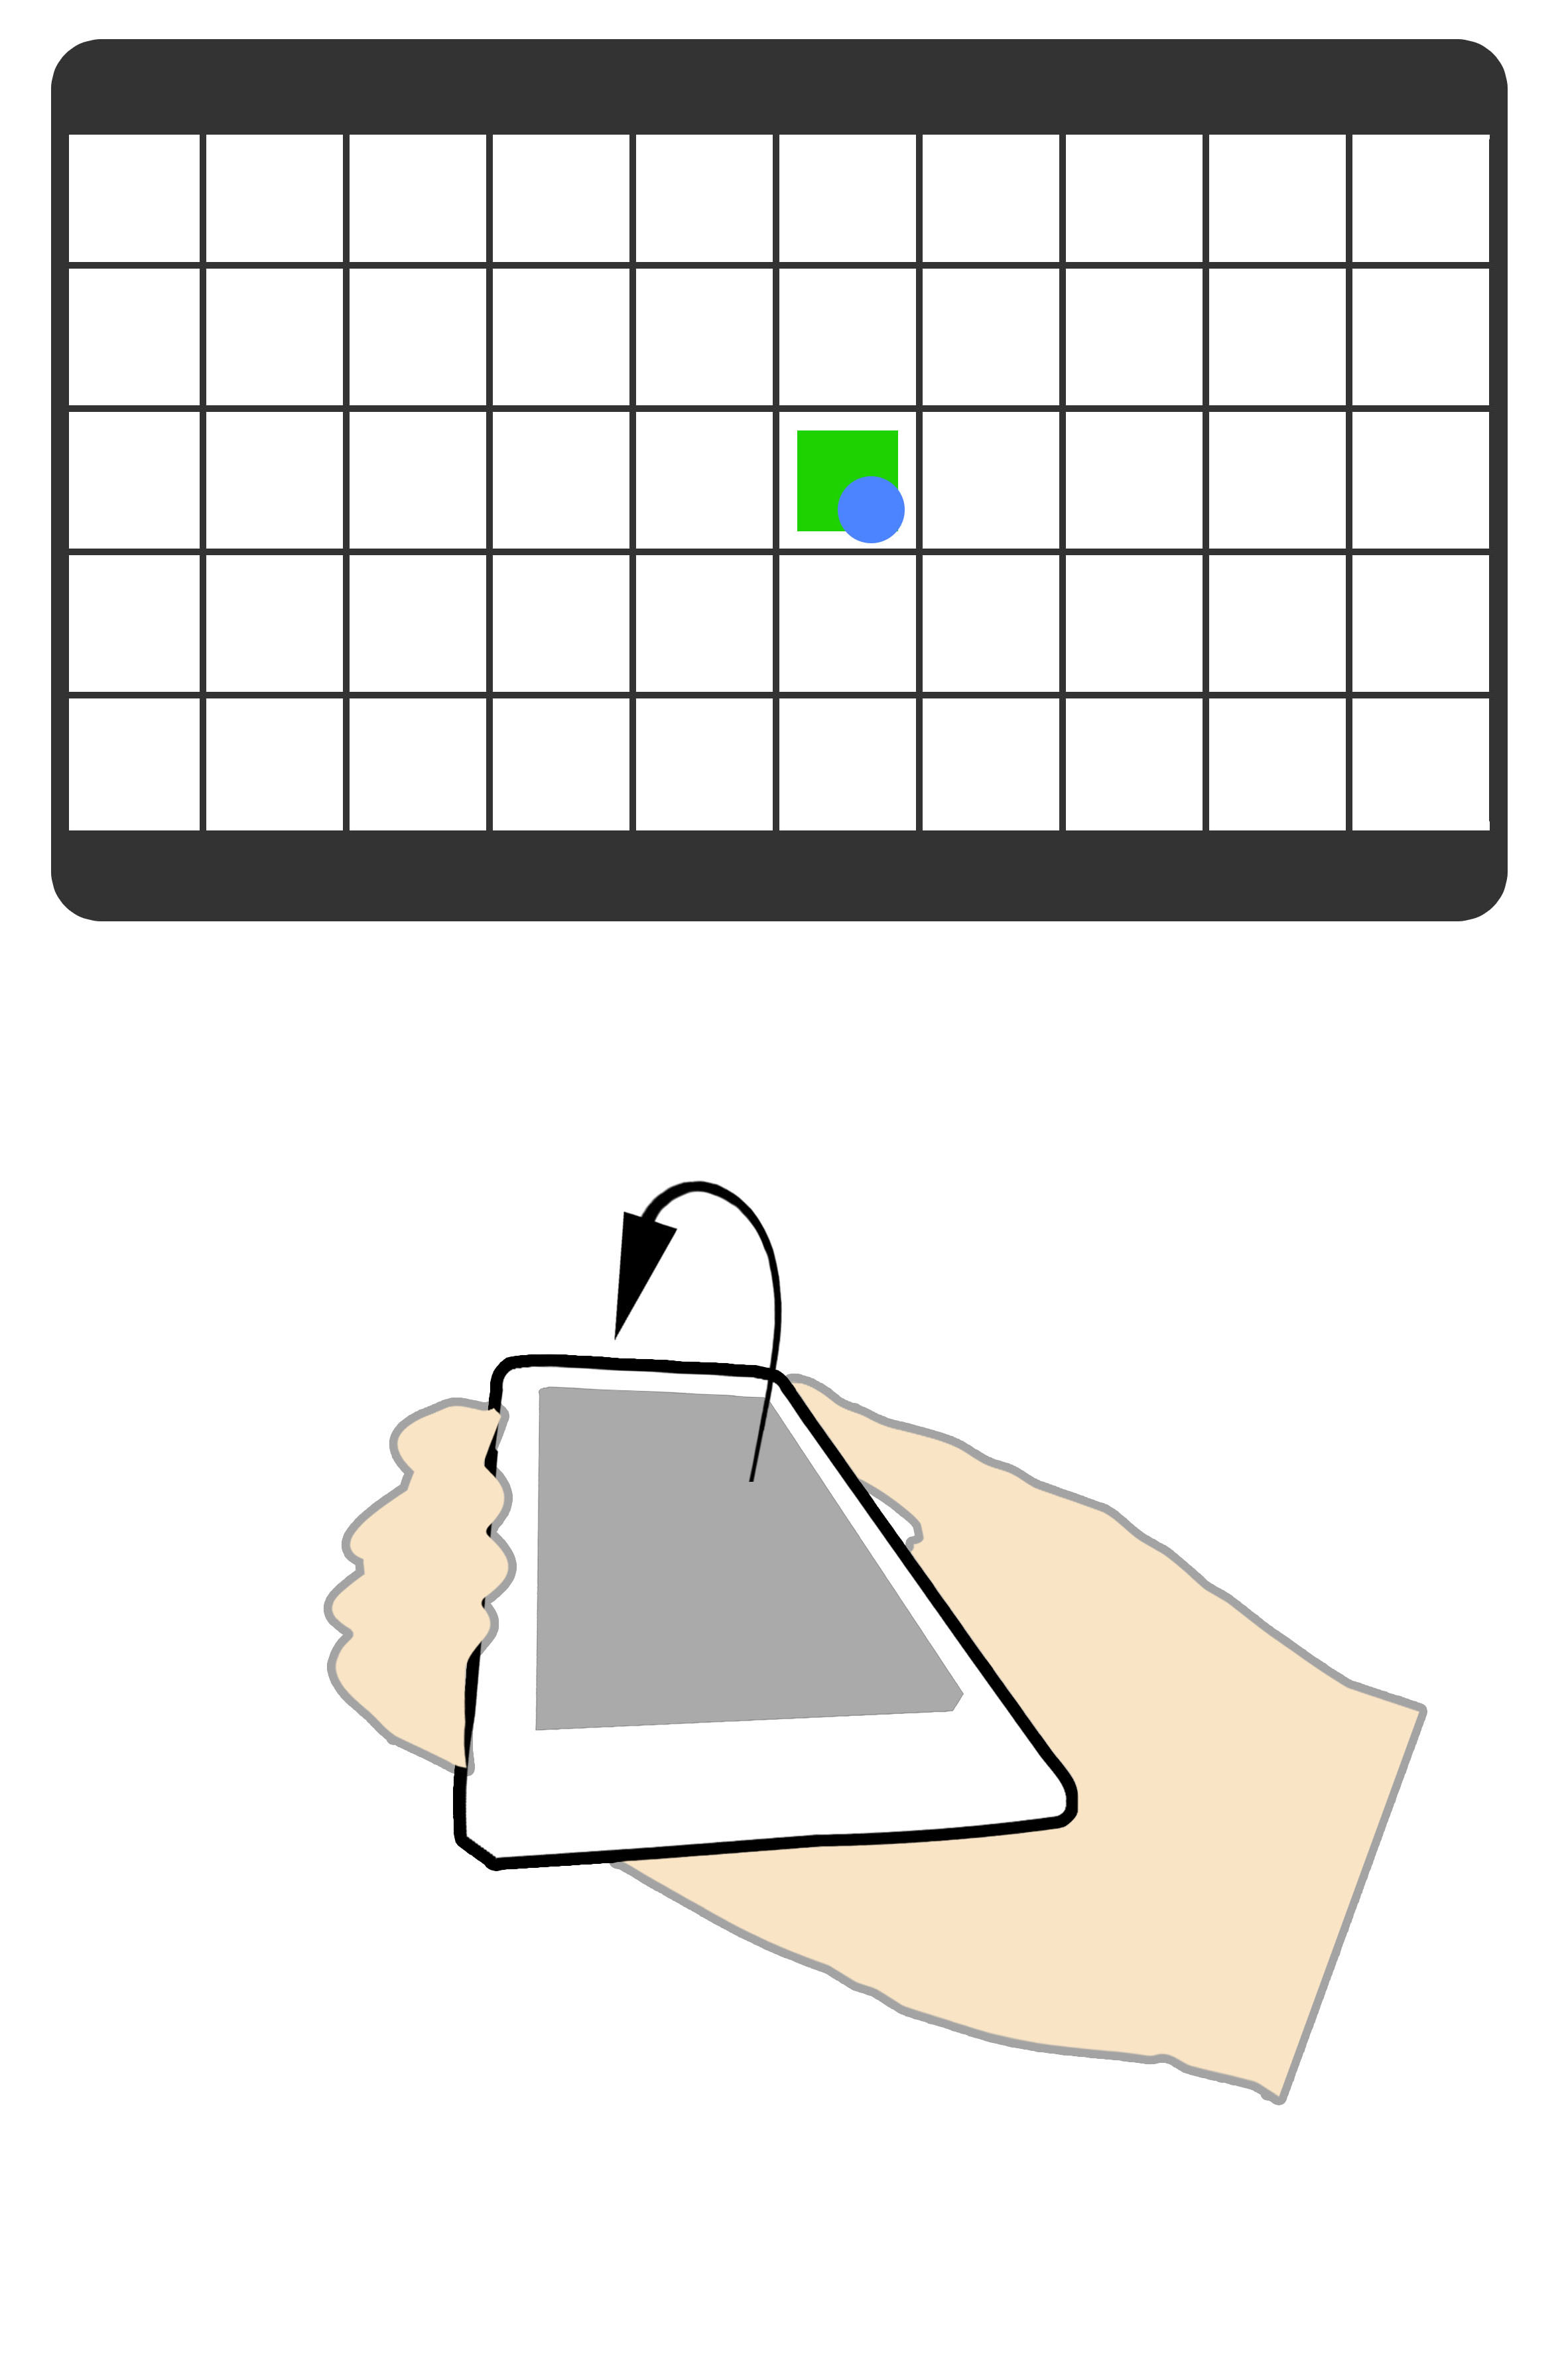
\includegraphics[width = 0.33\columnwidth]{images/techniques/tiltPush3.jpg}\label{fig:tiltPush3}}
	\caption{\push \grab technique}
	\label{fig:grabTechnique}
\end{figure}
\cleardoublepage

% !TEX root = ../report.tex
\section*{Concluding Remarks} \label{sec:conclusion}
\addcontentsline{toc}{section}{Concluding Remarks}

This thesis deals with the theme of cross-device interaction between mobile devices and large displays. 
We approached this theme by finding and implementing 8 different interaction techniques and then performing a comparative study between them.

One of the ideas behind this thesis was to see if we could find any attributes to these techniques that made them successful in regards to accuracy and efficiency.
We initially believed that the some of the important attributes to the success of a technique would be whether or not the phone was in motion during the technique and the amount of hands used to perform the given technique.

Our results did show that there might be some association between the amount of hands and the accuracy and efficiency of each technique. 
There seems to be some indication that one handed techniques are faster to perform that two handed, but that two handed techniques are more accurate.
These are only indications though and in order to more conclusively say that this is indeed the case, more research must be conducted with these specific attributes in mind.  

A much more important attribute though came up and that was the ability to hold the cursor still while performing the technique. 
The two most successful techniques, \emph{Swipe} and \emph{Throw} both had that in common. 
Users where capable of keeping the cursor still while activating and performing the technique.
The other two techniques, \emph{Tilt} and \emph{Grab}, both movements on the cursor pointing hand, causing the cursor to move during activation instead of keeping it stable. 

In the future, we would like to extend our research by examining more closely the relationship between amount of hands and the efficiency and accuracy of each technique. 
This could be done by implementing different techniques were the focus is much more on the amount of hands and the role of each hand while performing the given technique.
Having techniques were the sole role of one of the hands is for aiming, like \emph{Throw}, and others were each hand has some gesture it has to perform in order to activate the technique, such as \emph{Grab}.
A research like this could lead to a much more clear understanding of how the amount of hands affects the performance of a interaction technique.
\cleardoublepage

\newpage\null\thispagestyle{empty}\newpage
\cleardoublepage

% Appendix start
\pagenumbering{Roman}
\setcounter{page}{1}
\pagestyle{appendixplain}

% Appendix TOC
\addtocontents{toc}{\protect\renewcommand{\protect\cftsecleader}{\hfill}}
\cftaddtitleline{toc}{section}{Appendices}{}
\includepdf[pages=-,pagecommand={\thispagestyle{customplain}}]{docs/appendix/appendix.pdf}

\newpage\null\thispagestyle{empty}\newpage
\cleardoublepage

% Appendix input start
\subsection*{\pictures}
\addcontentsline{toc}{subsection}{\pictures}

\subsection*{Setup}
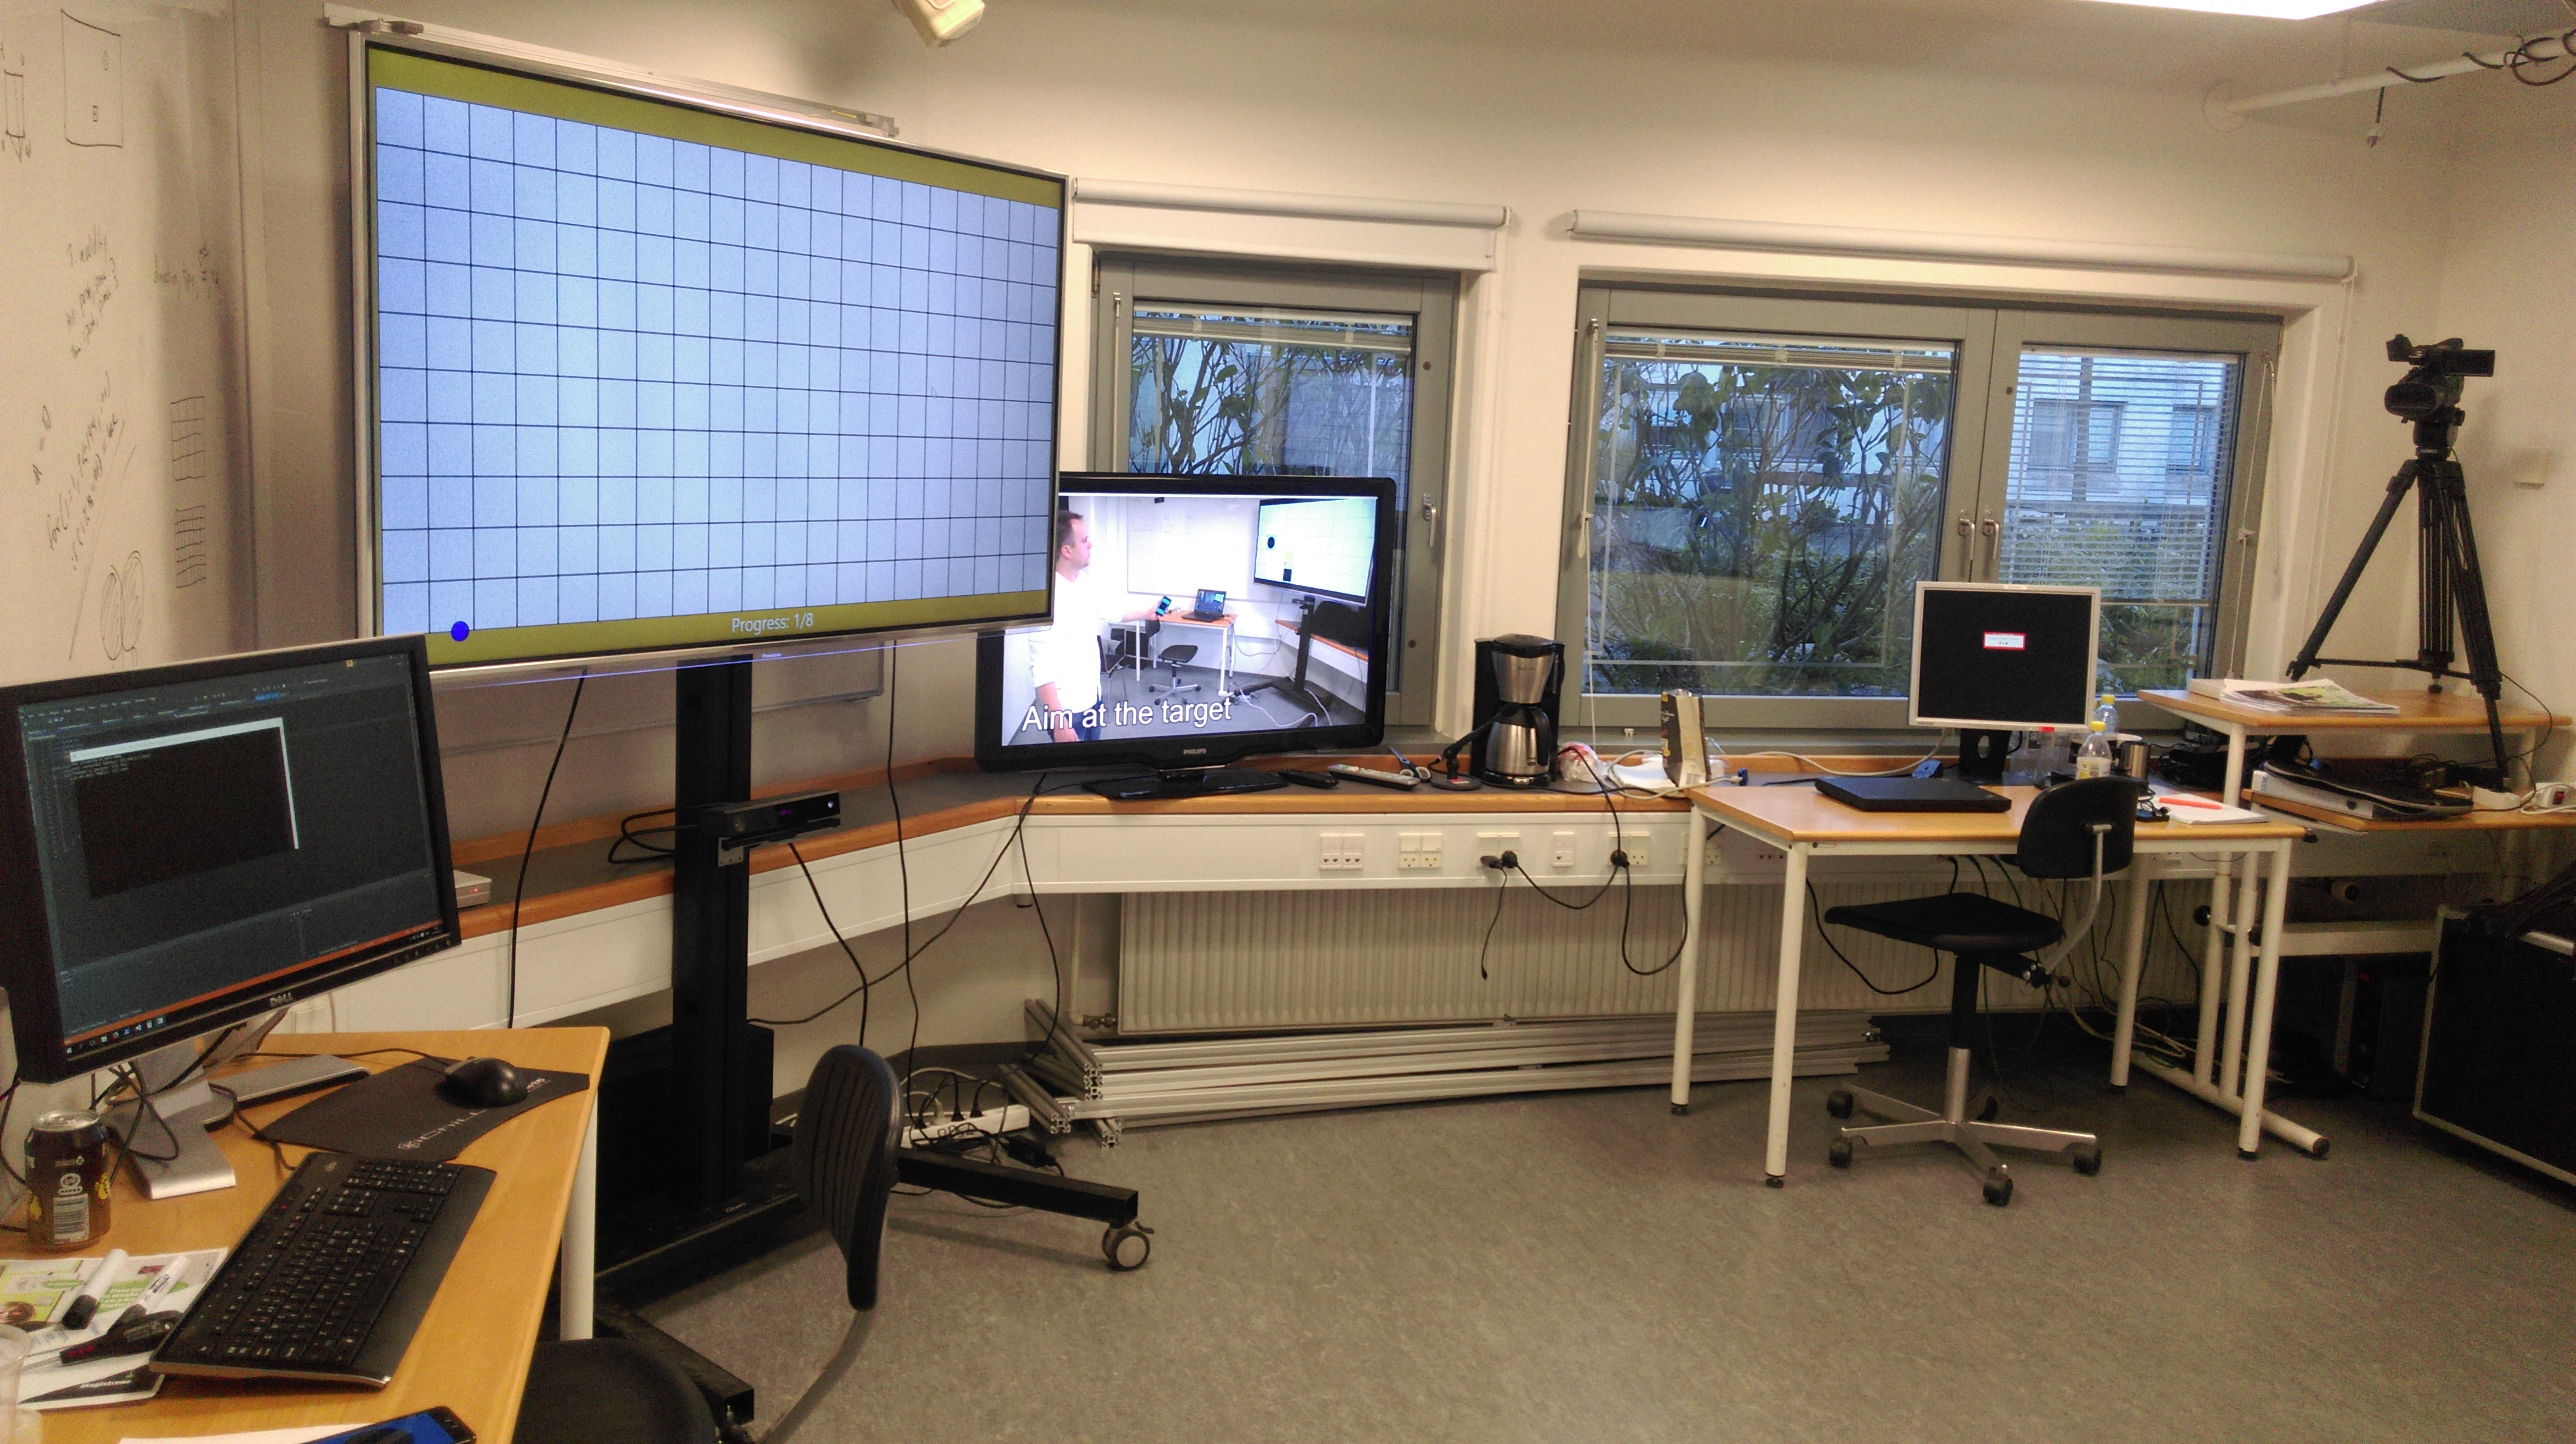
\includegraphics[width=\textwidth]{docs/appendix/files/setup_left.jpg}
\\\\
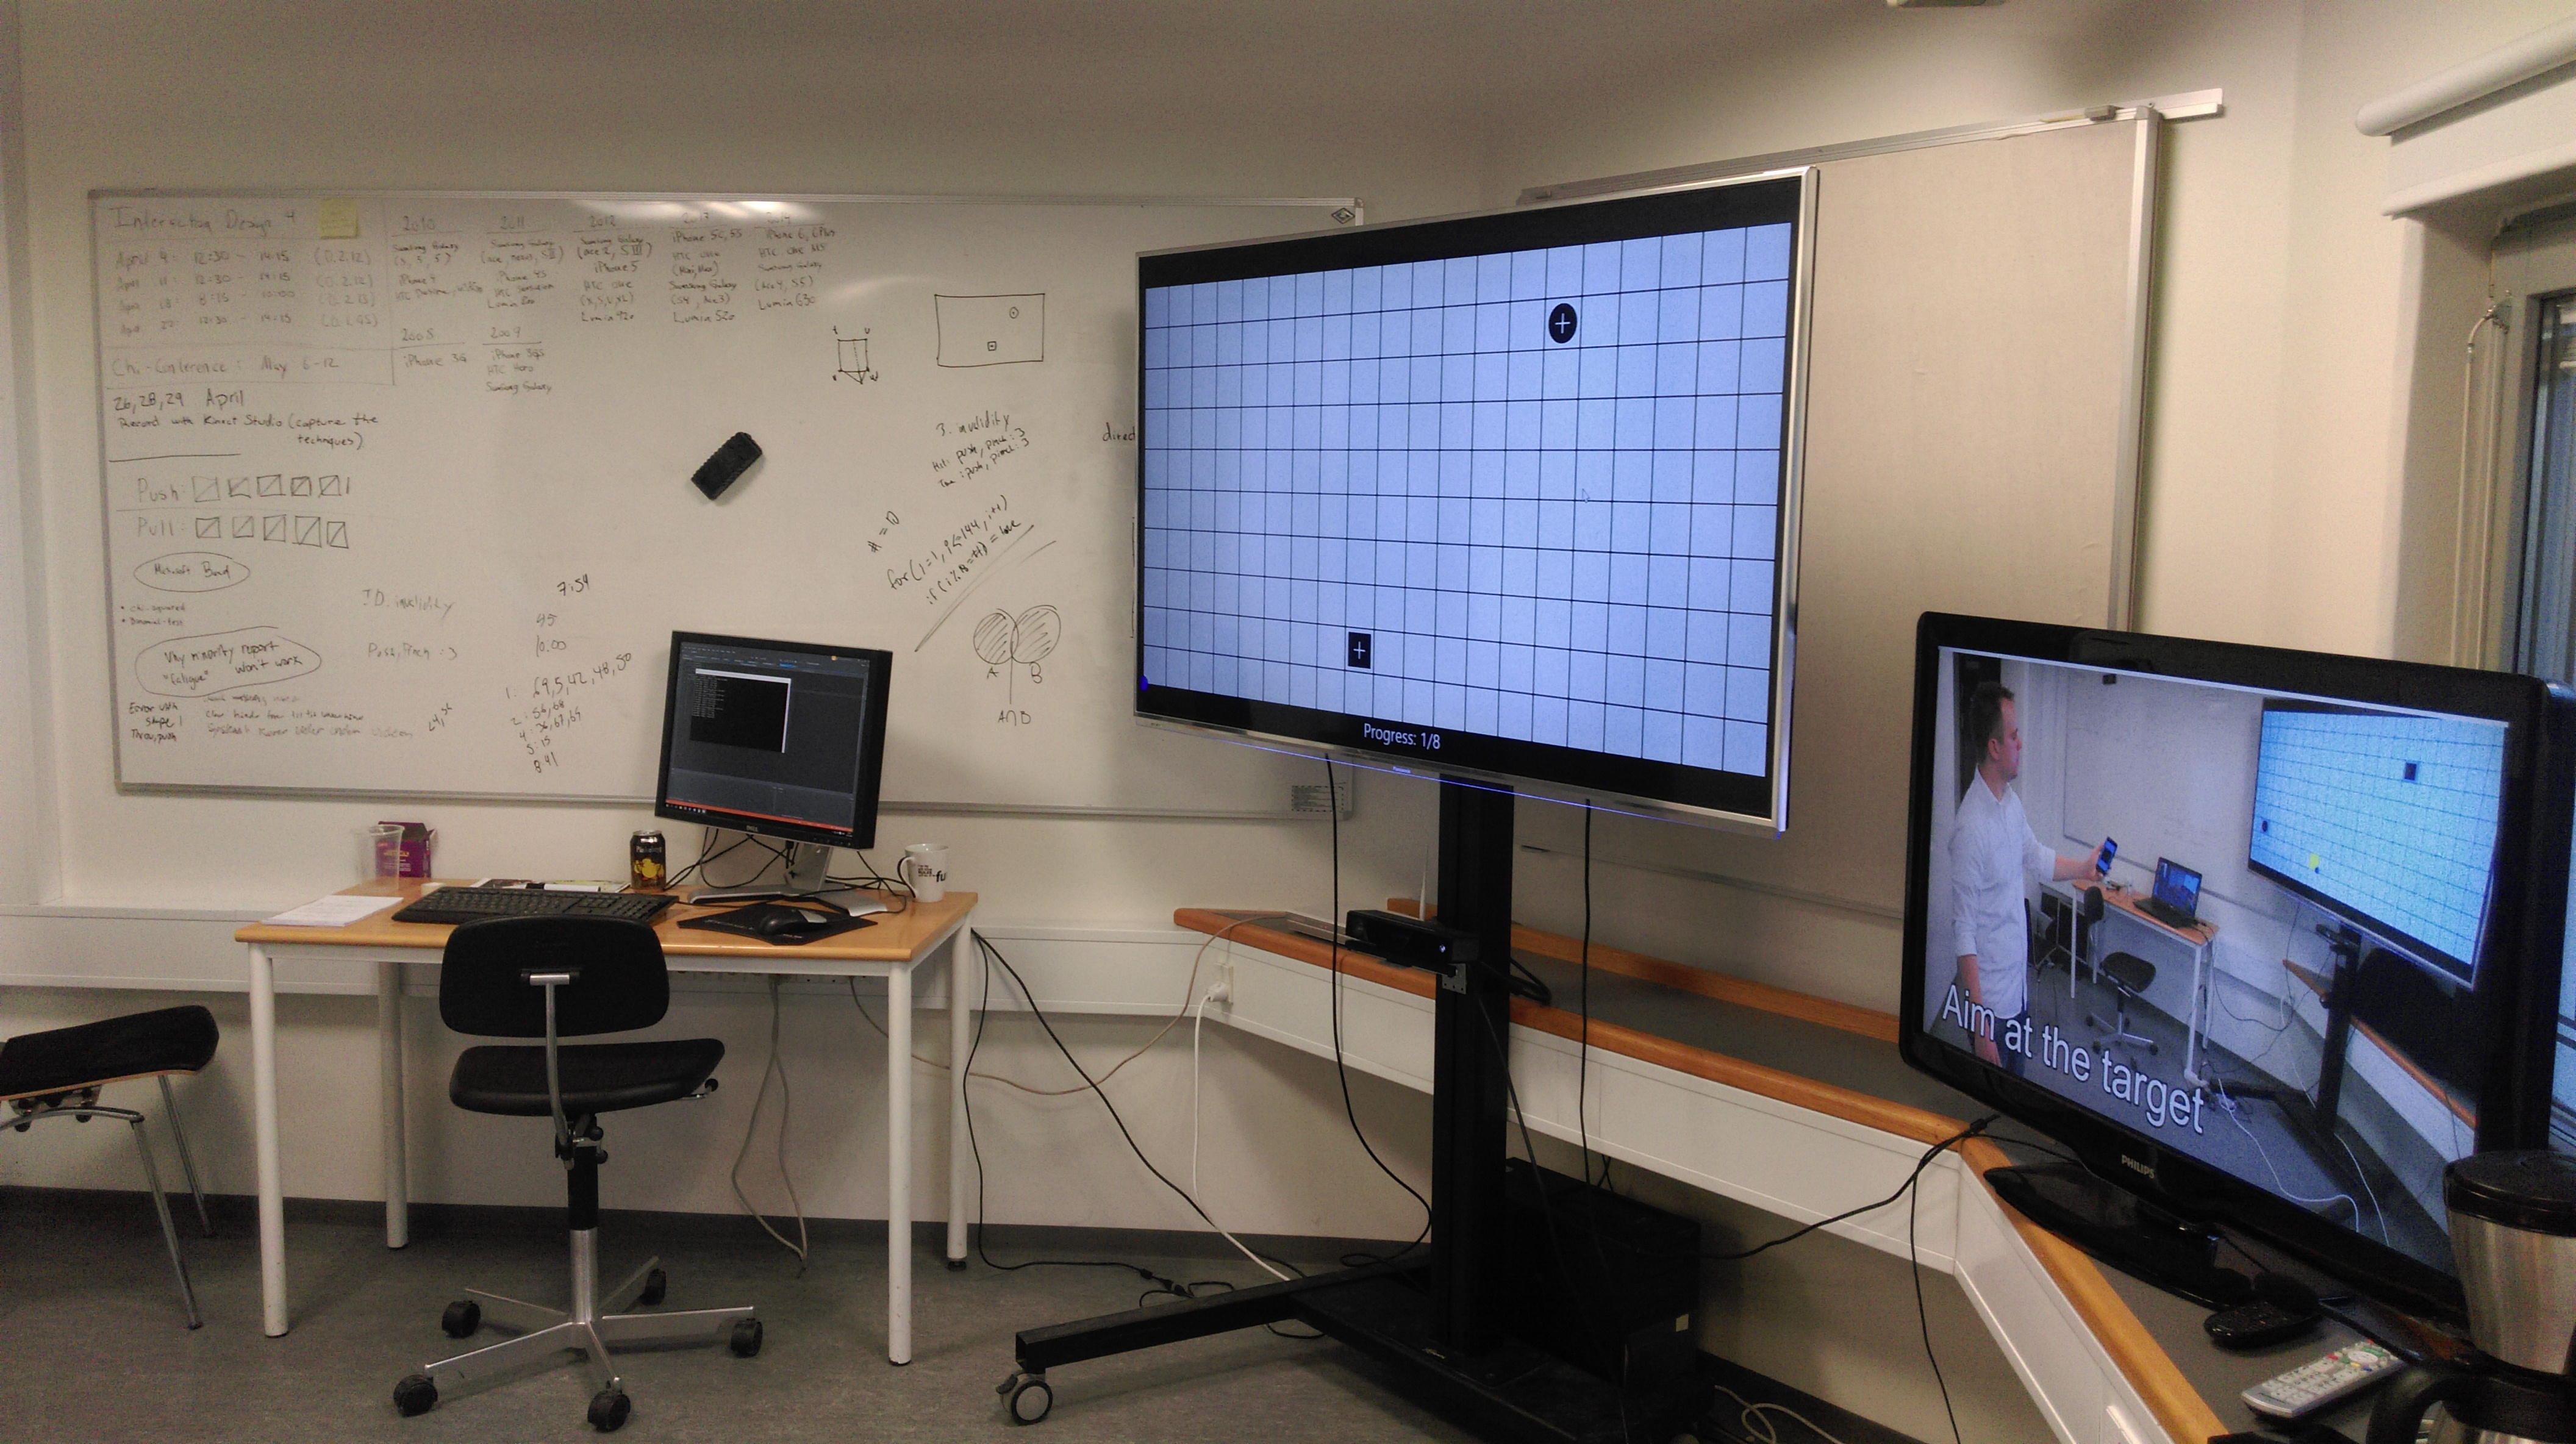
\includegraphics[width=\textwidth]{docs/appendix/files/setup_right.jpg}

\subsection*{Presenting the experiment}
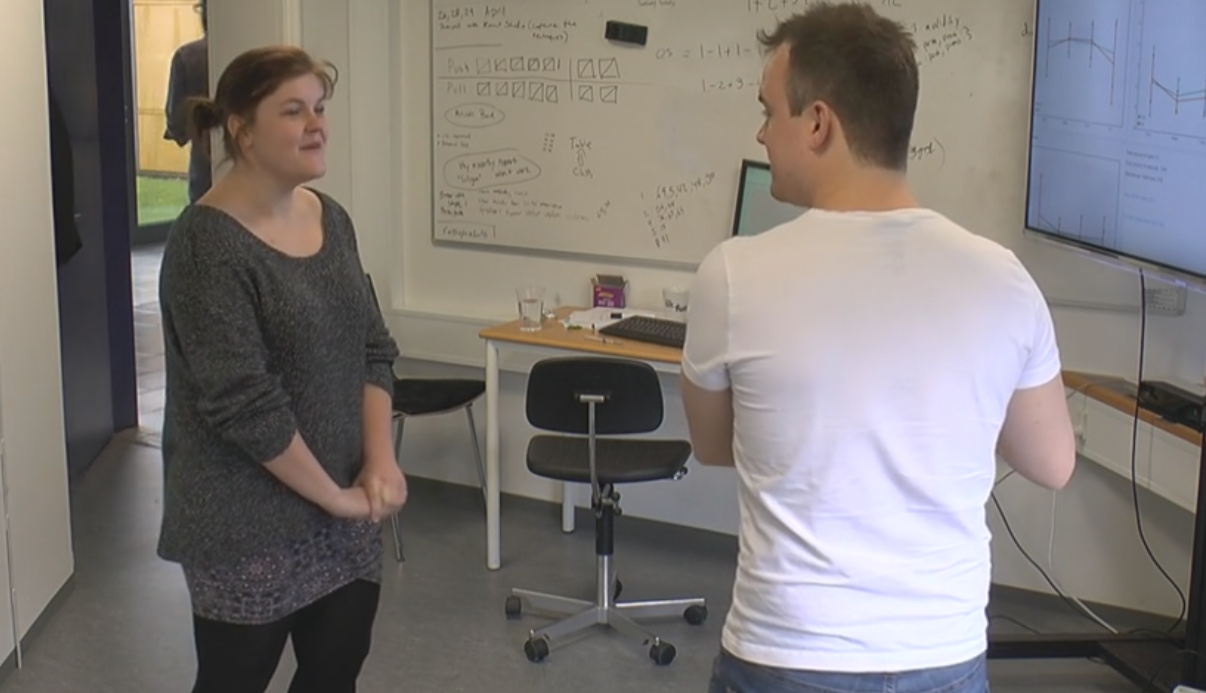
\includegraphics[width=\textwidth]{docs/appendix/files/introduction.png}

\subsection*{Discussing the experiment}
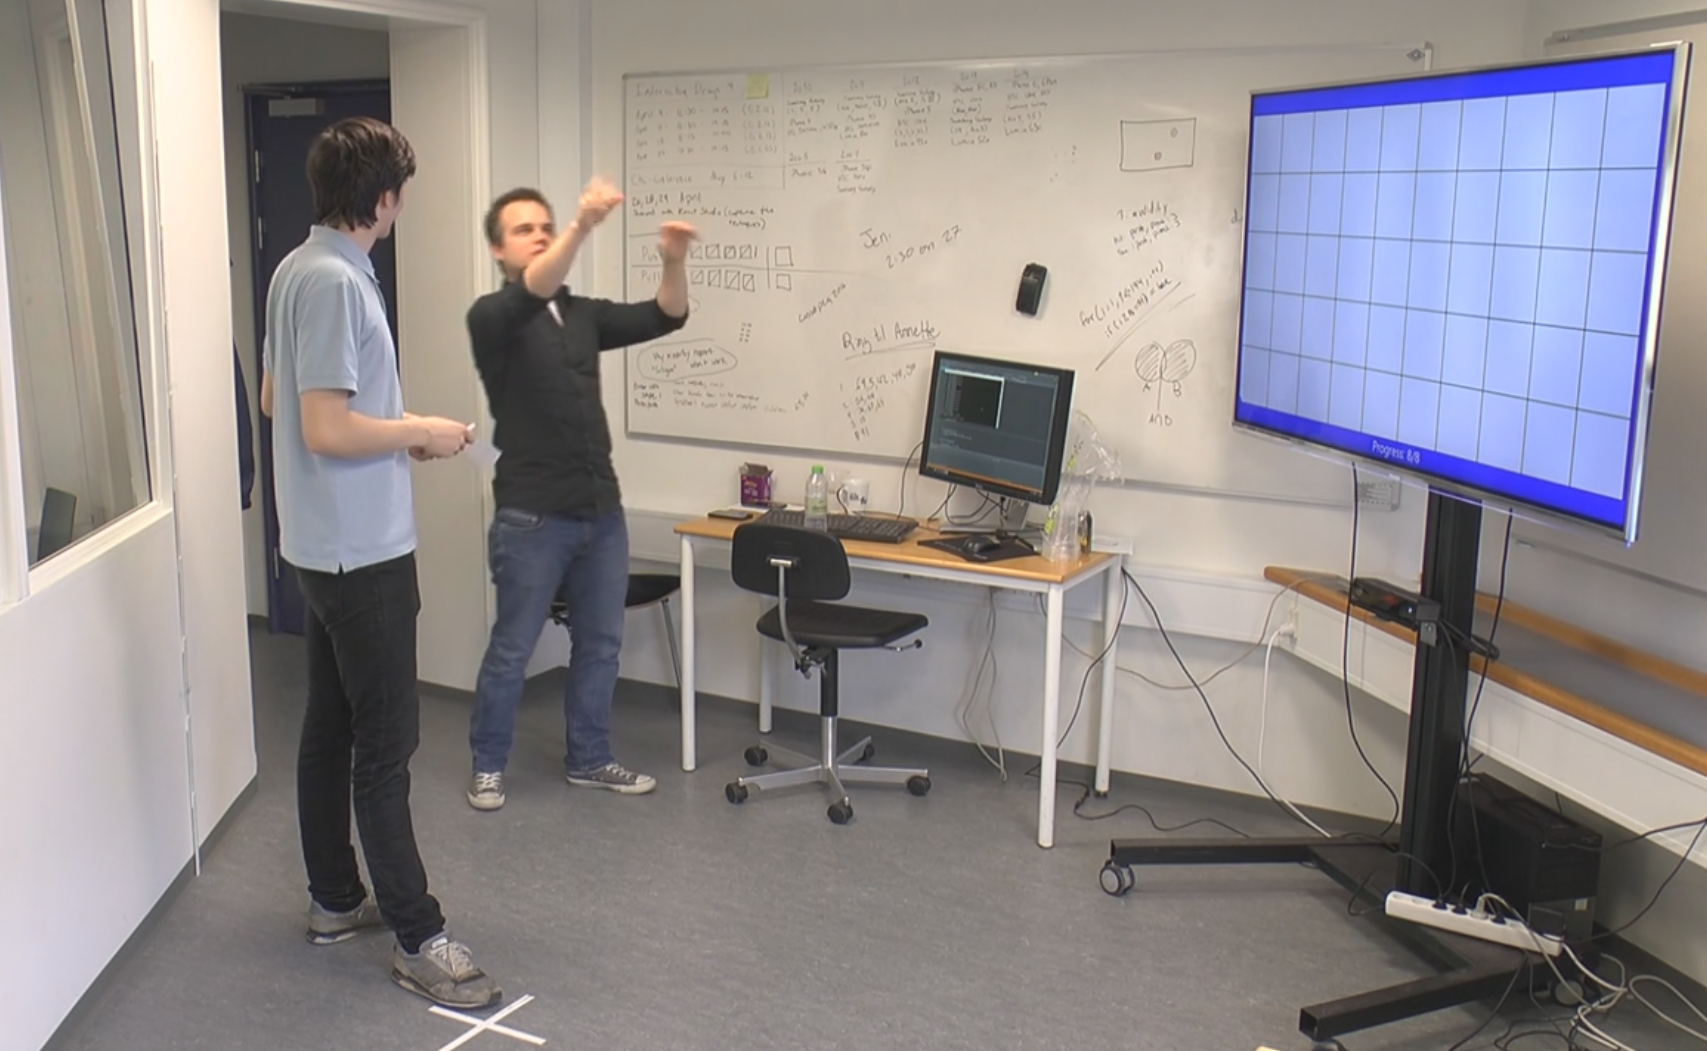
\includegraphics[width=\textwidth]{docs/appendix/files/discussion.png}

\subsection*{Grab technique}
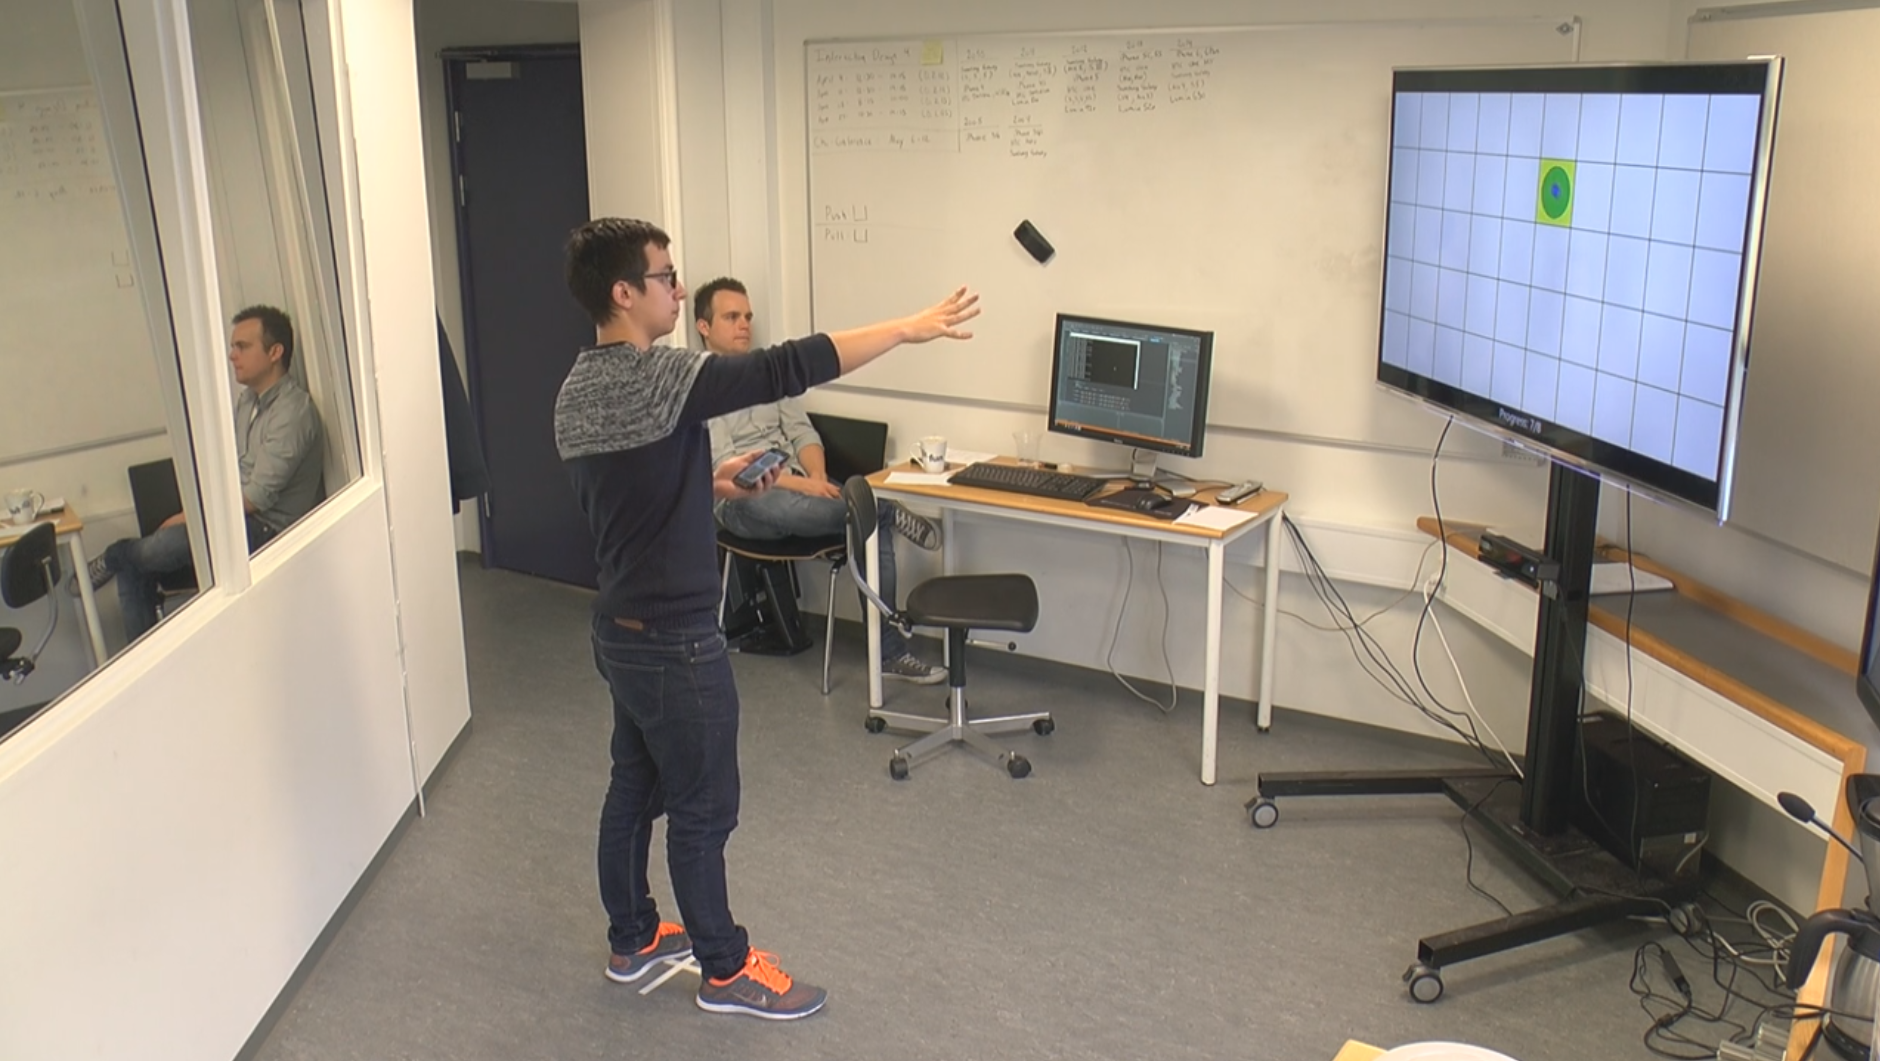
\includegraphics[width=\textwidth]{docs/appendix/files/grab_push.png}
\\ \vspace{1cm}
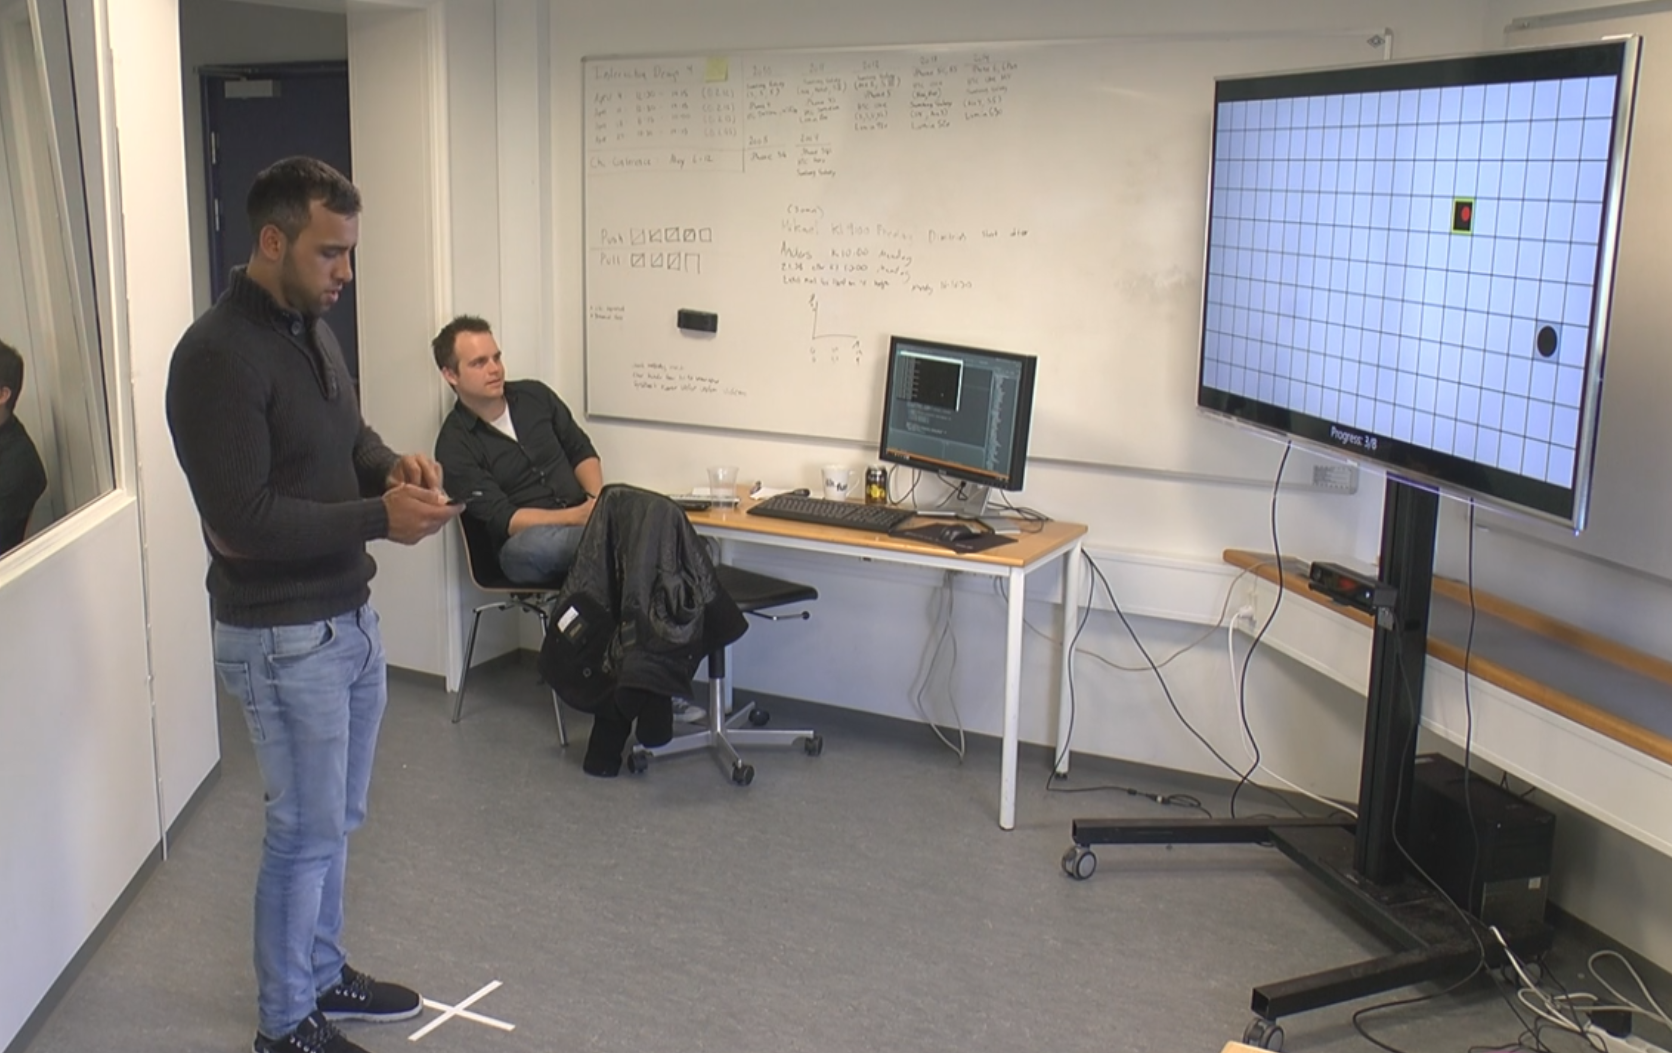
\includegraphics[width=\textwidth]{docs/appendix/files/grab_pull.png}

\subsection*{Swipe technique}
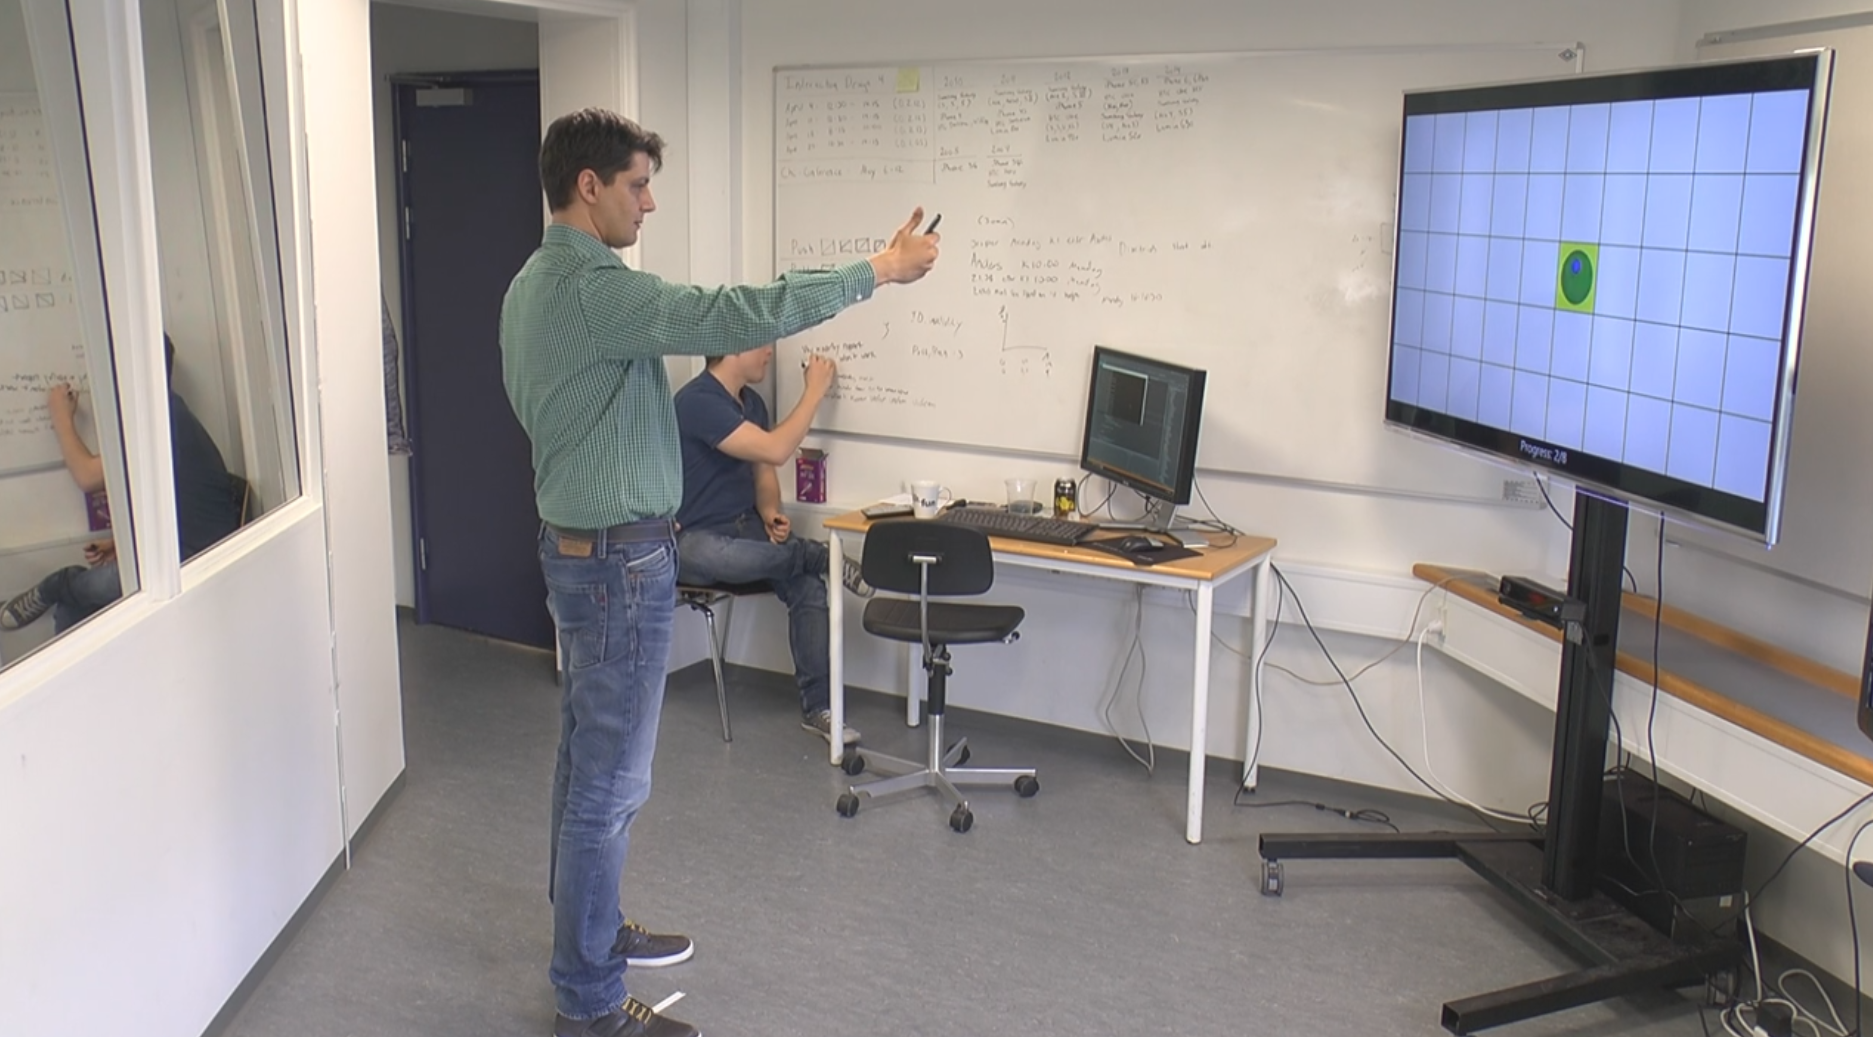
\includegraphics[width=\textwidth]{docs/appendix/files/swipe_push.png}
\\ \vspace{1cm}
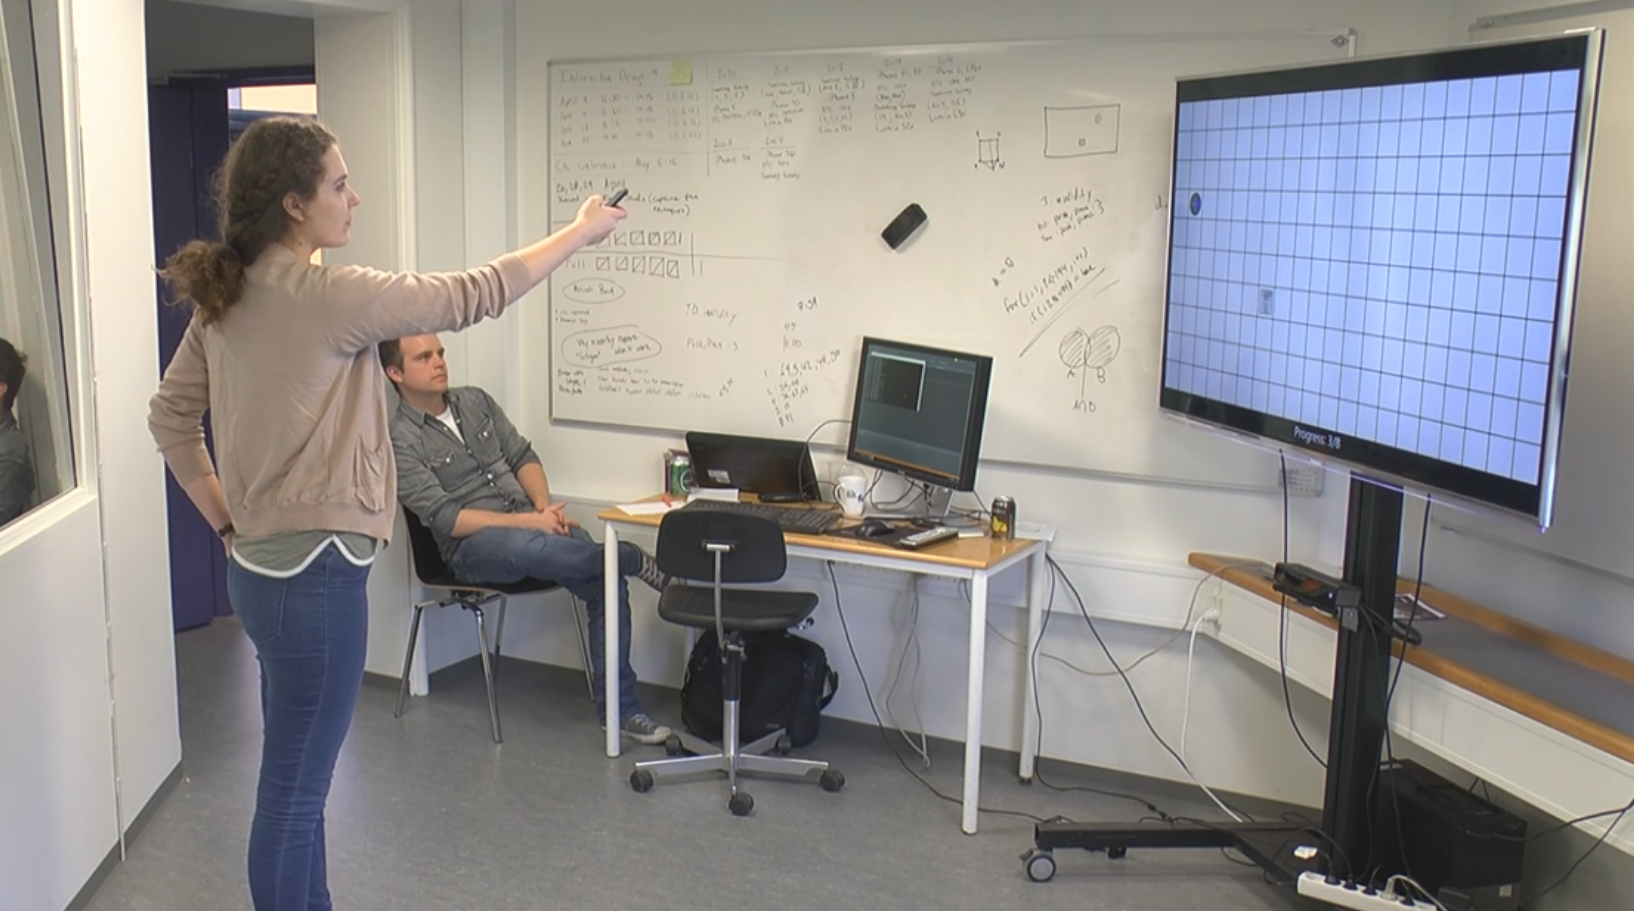
\includegraphics[width=\textwidth]{docs/appendix/files/swipe_pull.png}

\subsection*{Throw technique}
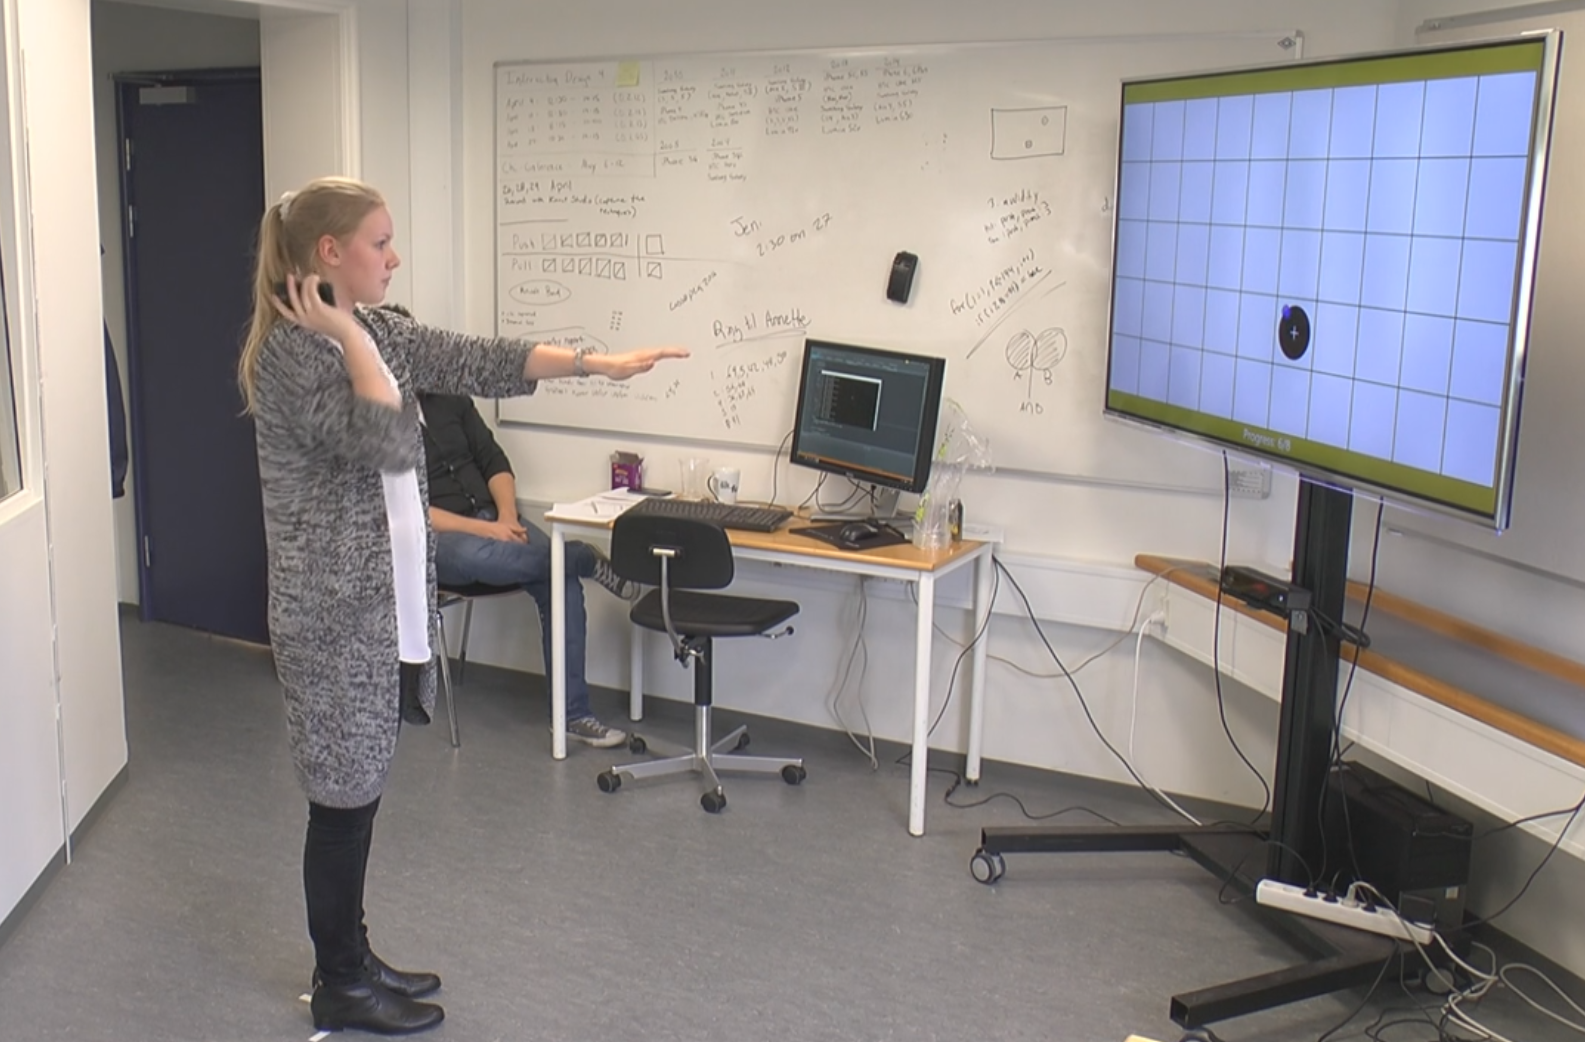
\includegraphics[width=\textwidth]{docs/appendix/files/throw_push.png}
\\ \vspace{1cm}
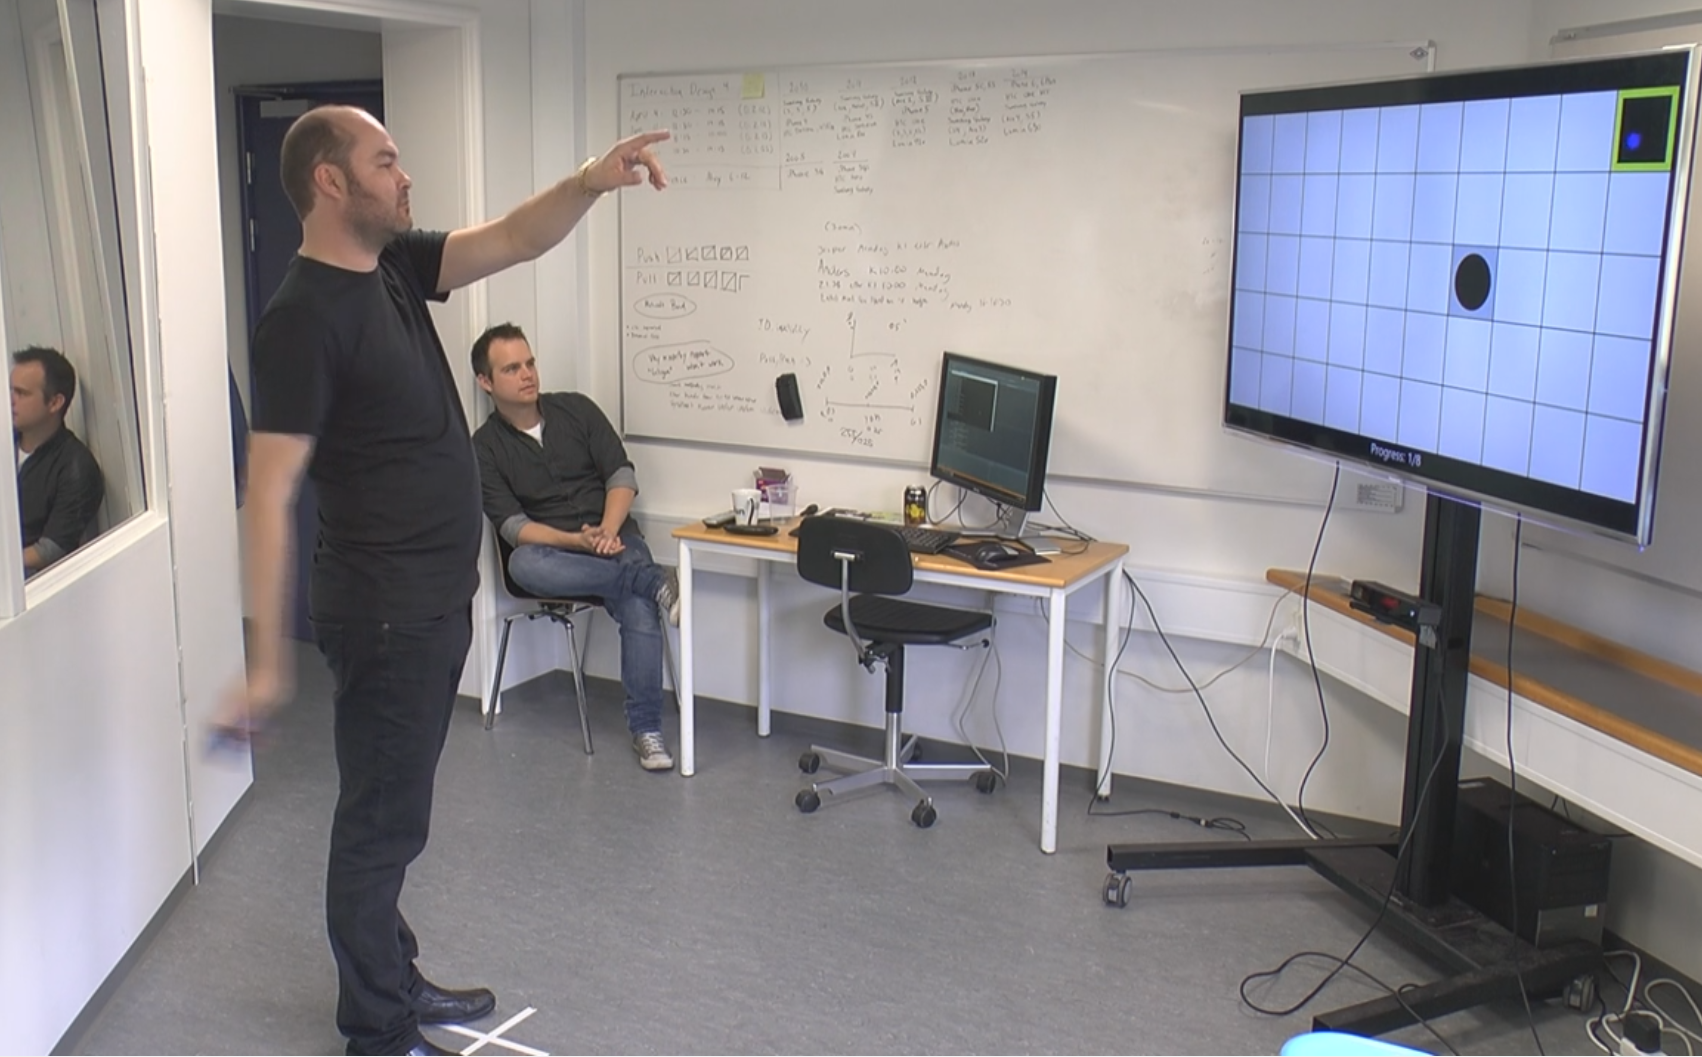
\includegraphics[width=\textwidth]{docs/appendix/files/throw_pull.png}

\subsection*{Tilt technique}
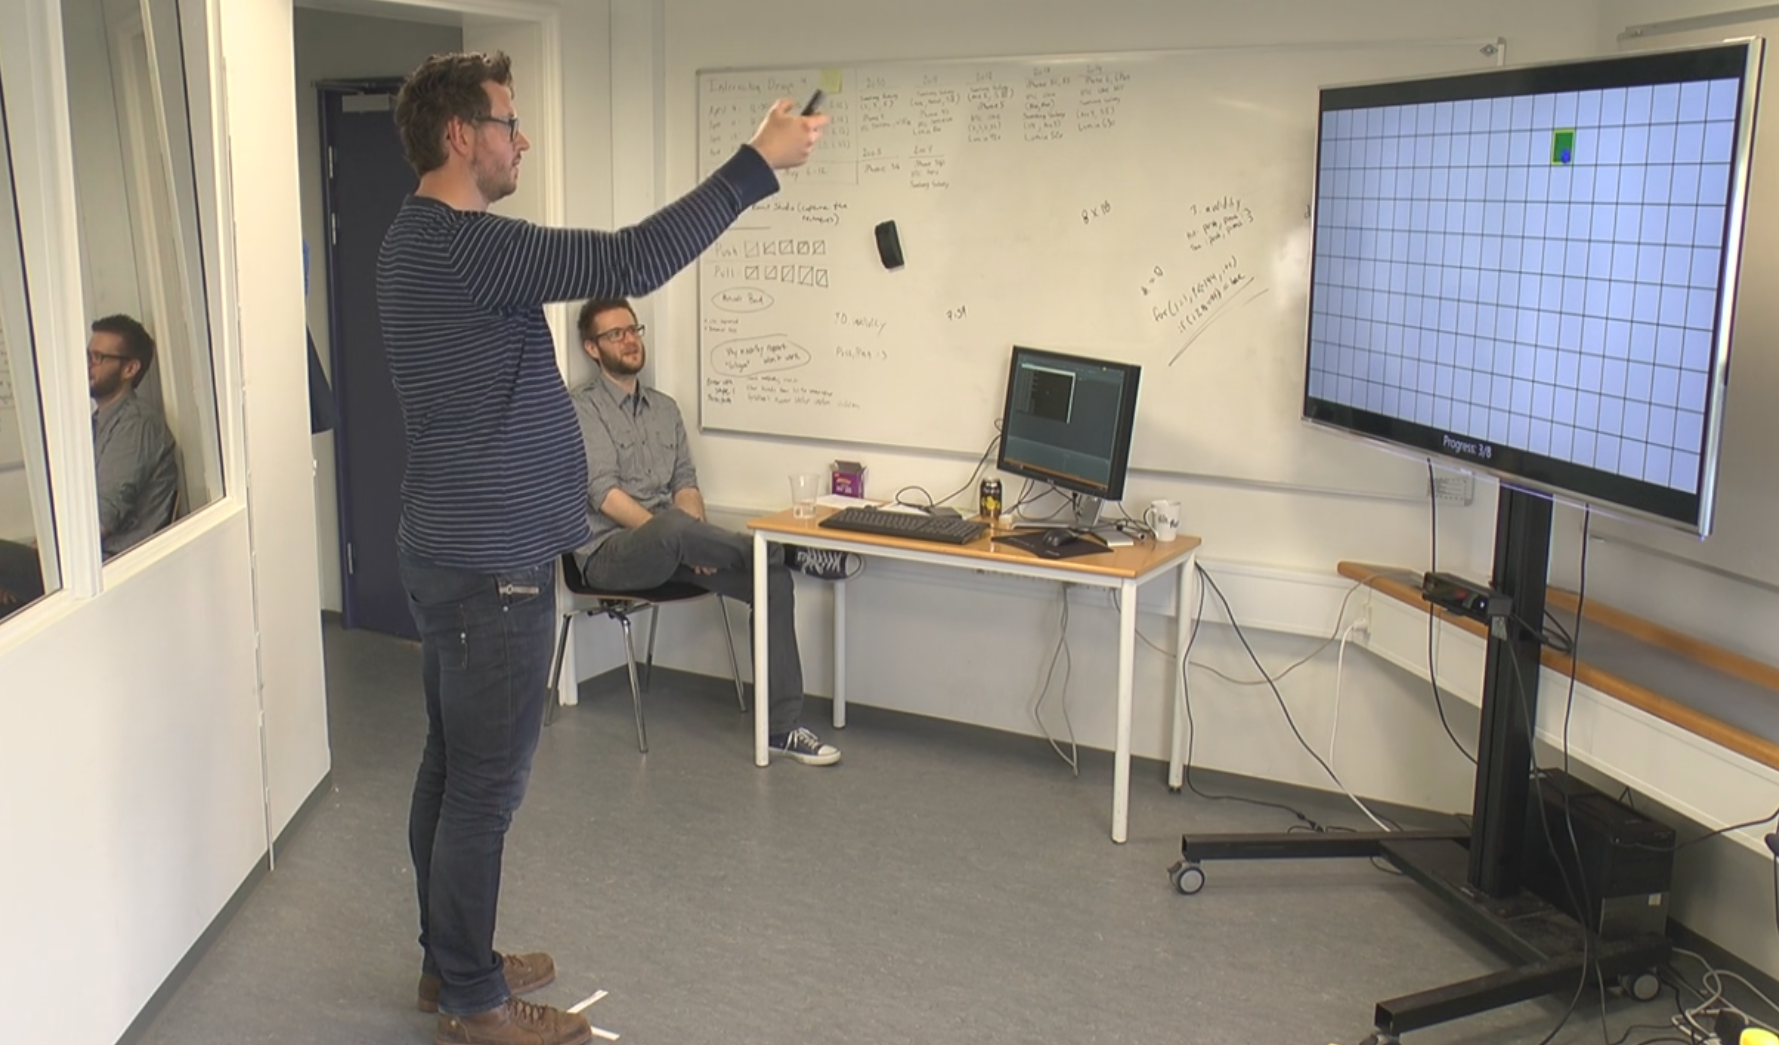
\includegraphics[width=\textwidth]{docs/appendix/files/tilt_push.png}
\\ \vspace{1cm}
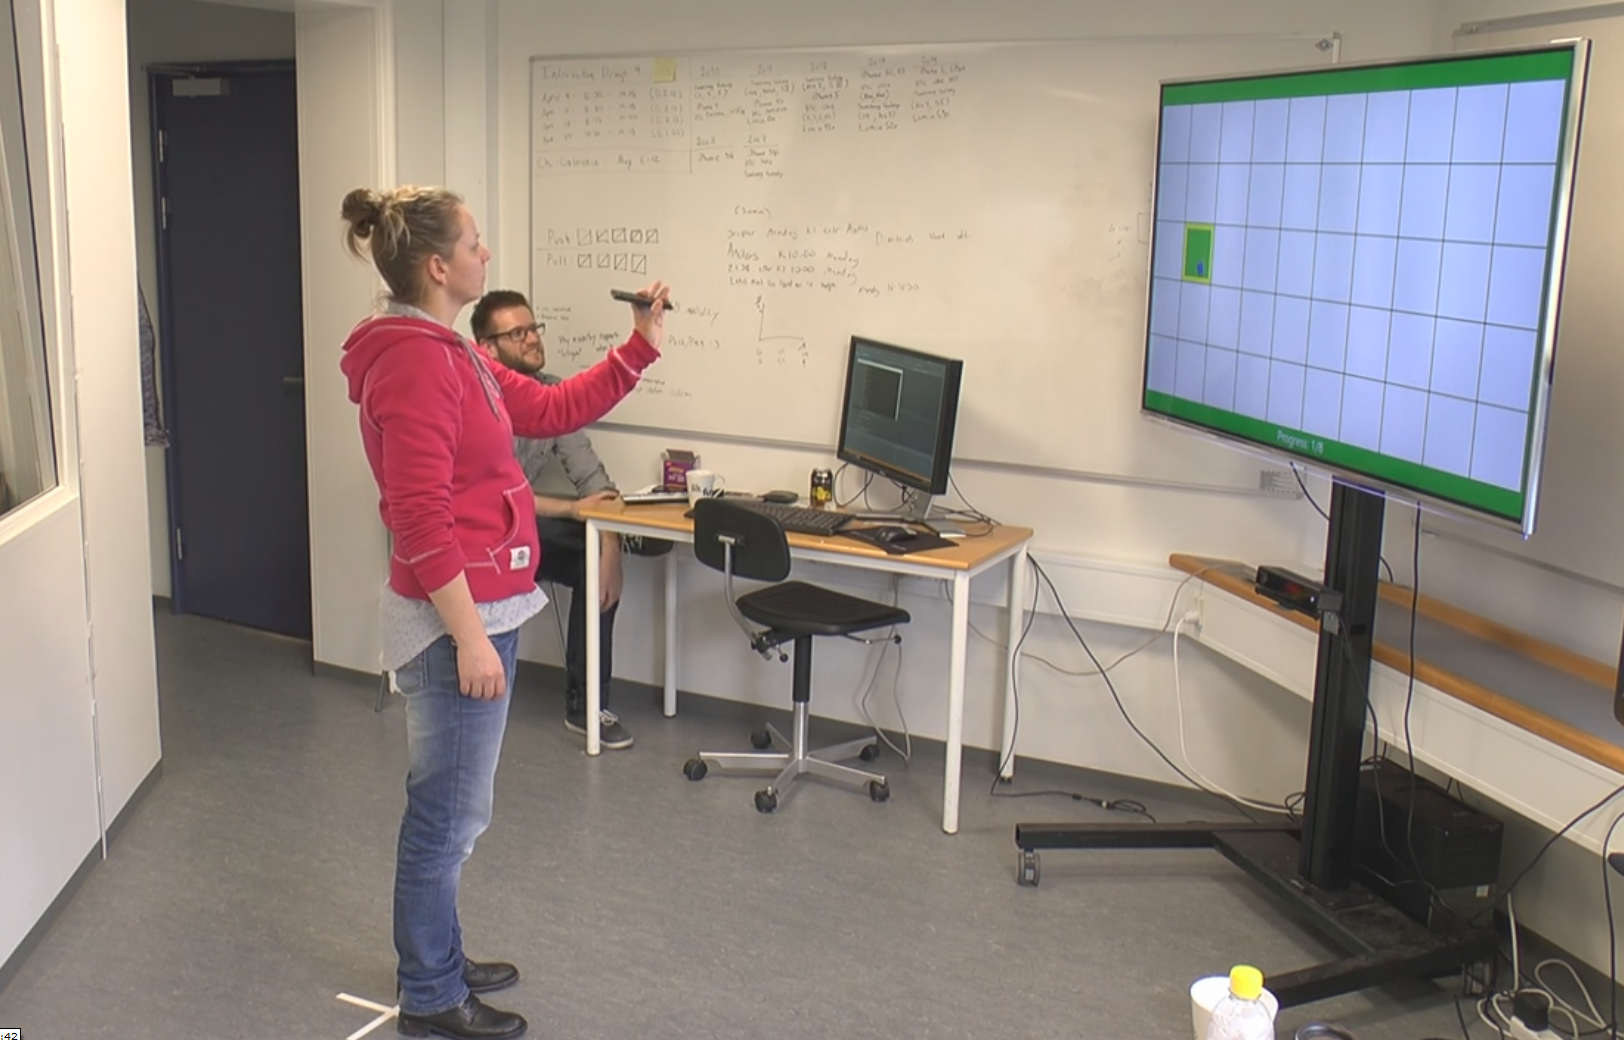
\includegraphics[width=\textwidth]{docs/appendix/files/tilt_pull.png}

\subsection*{Class observer}
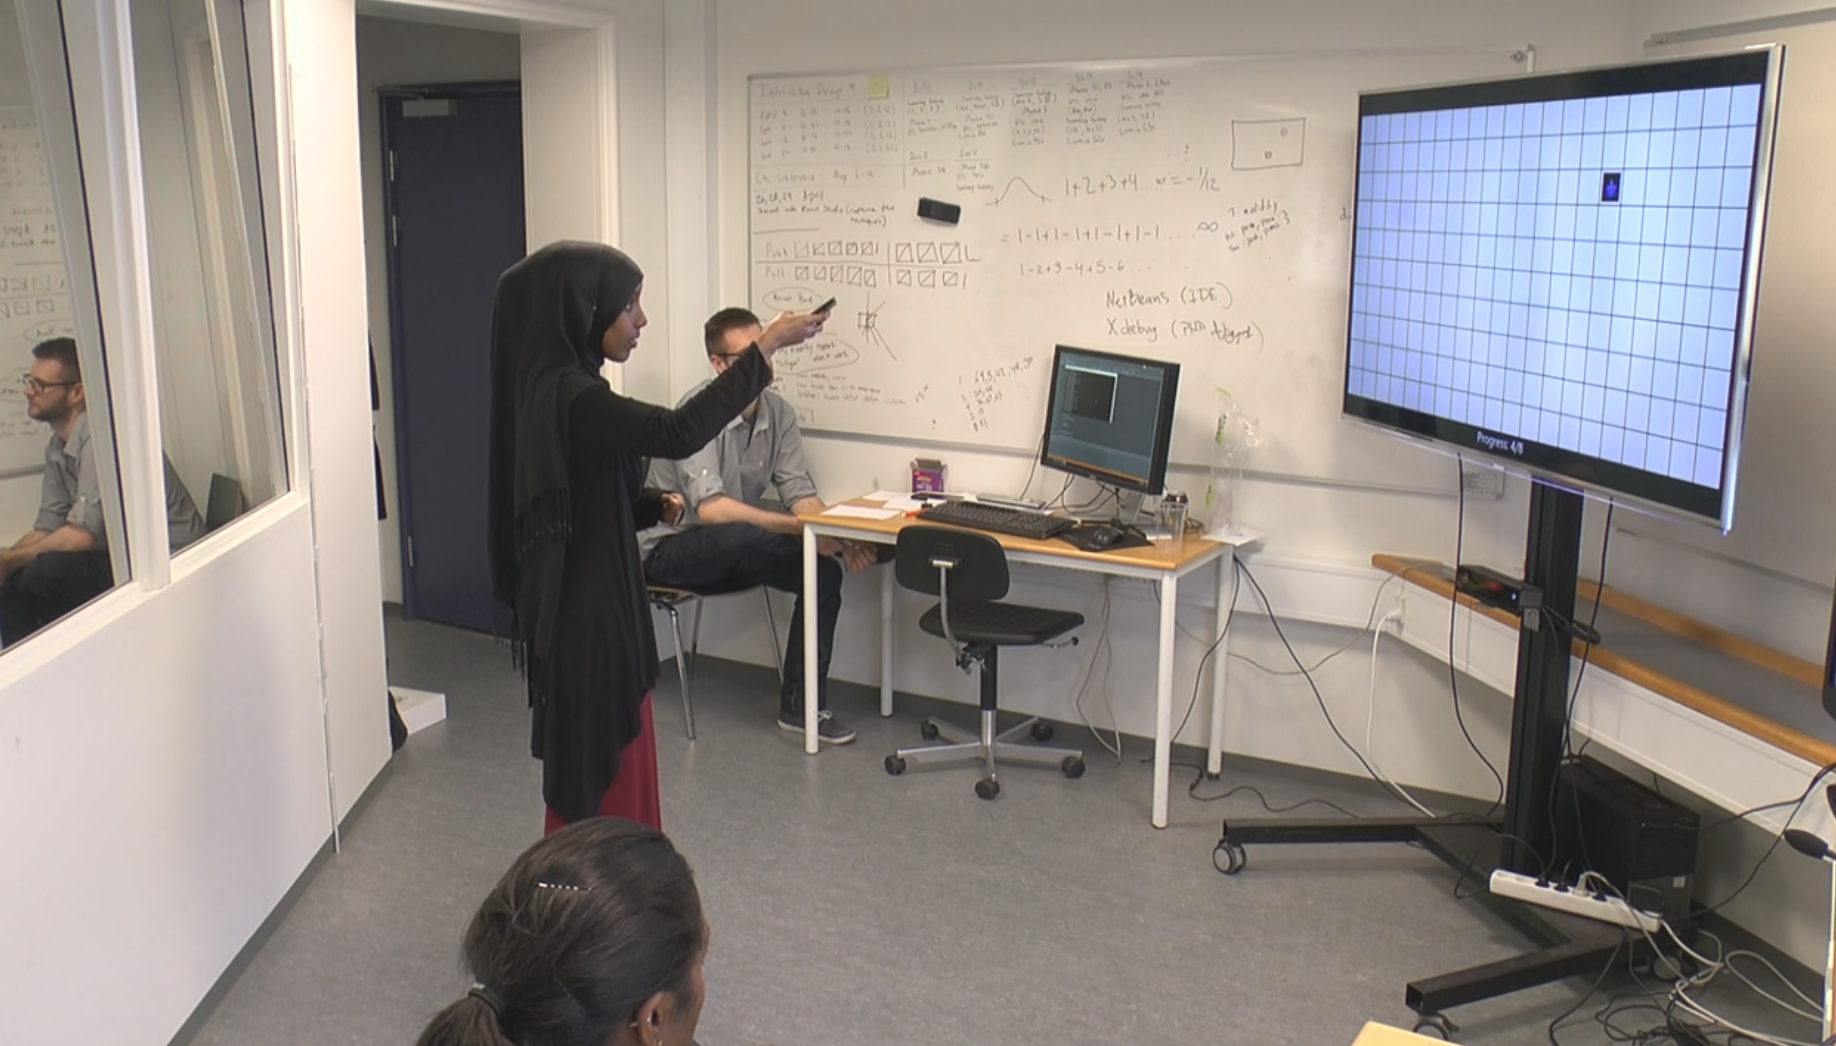
\includegraphics[width=\textwidth]{docs/appendix/files/class_observer.png}

\subsection*{Accuracy study}
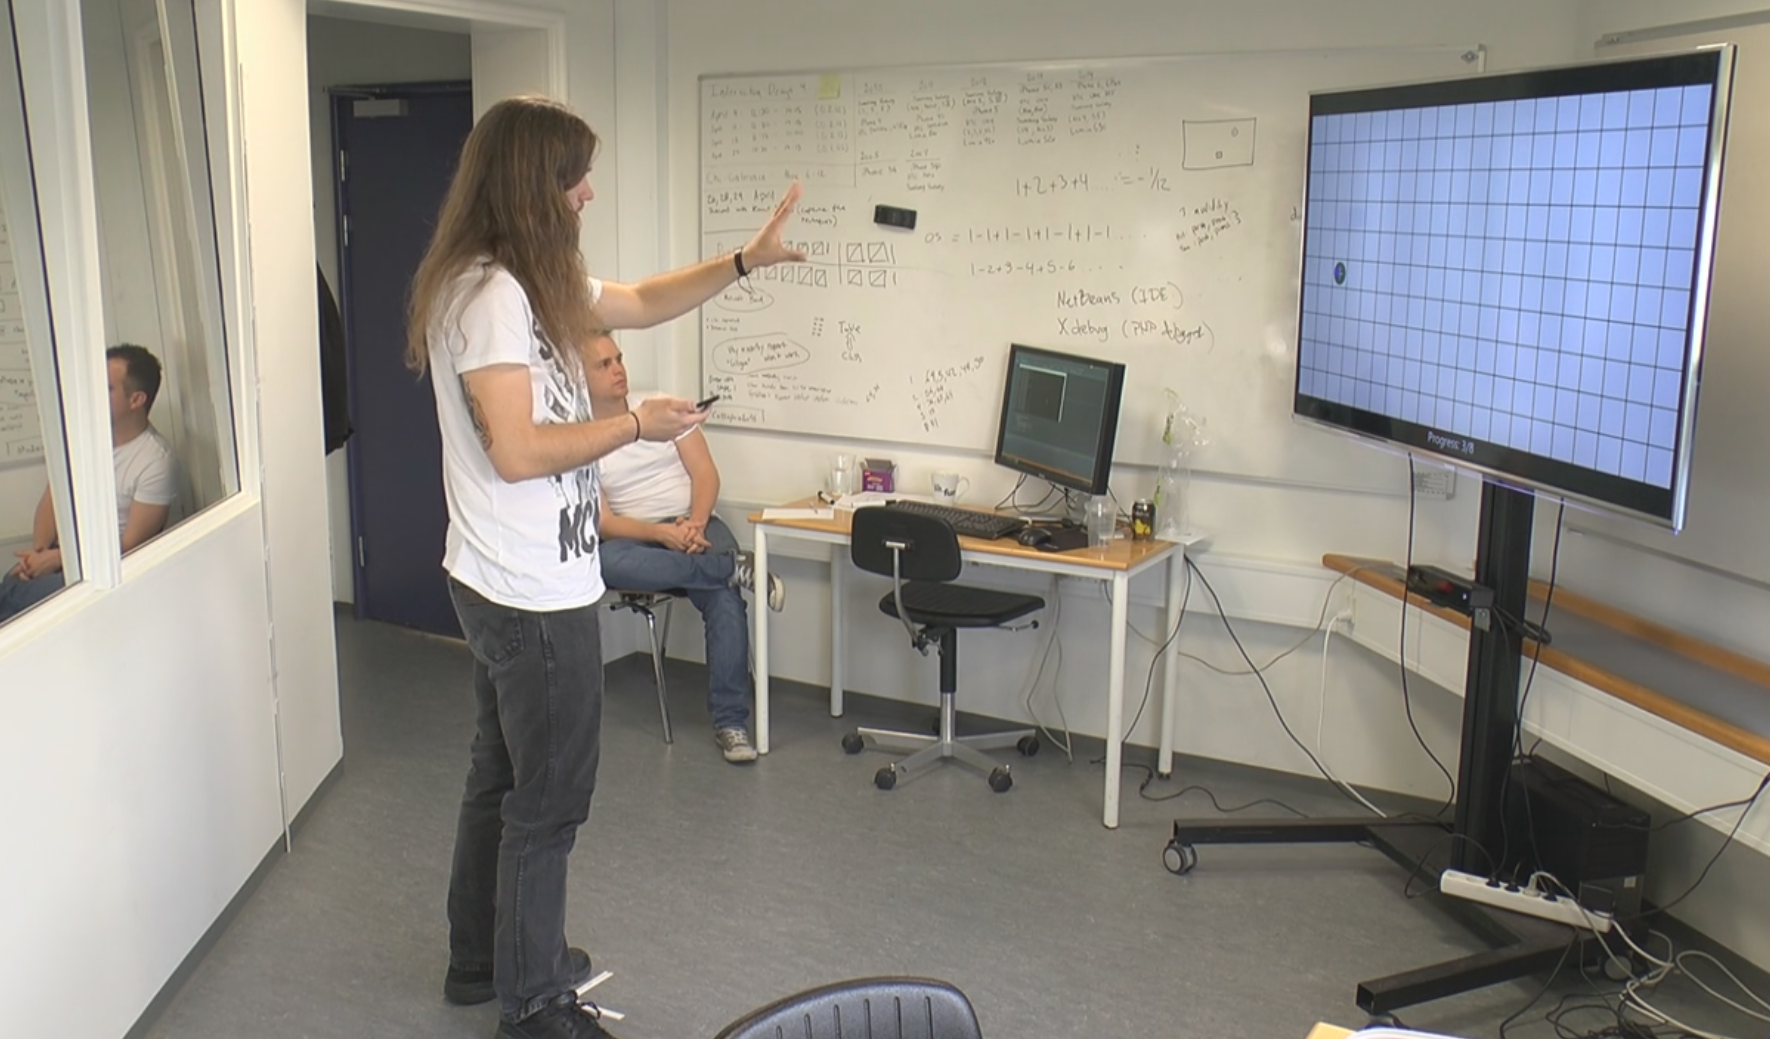
\includegraphics[width=\textwidth]{docs/appendix/files/accuracy.png}

\addbackpage
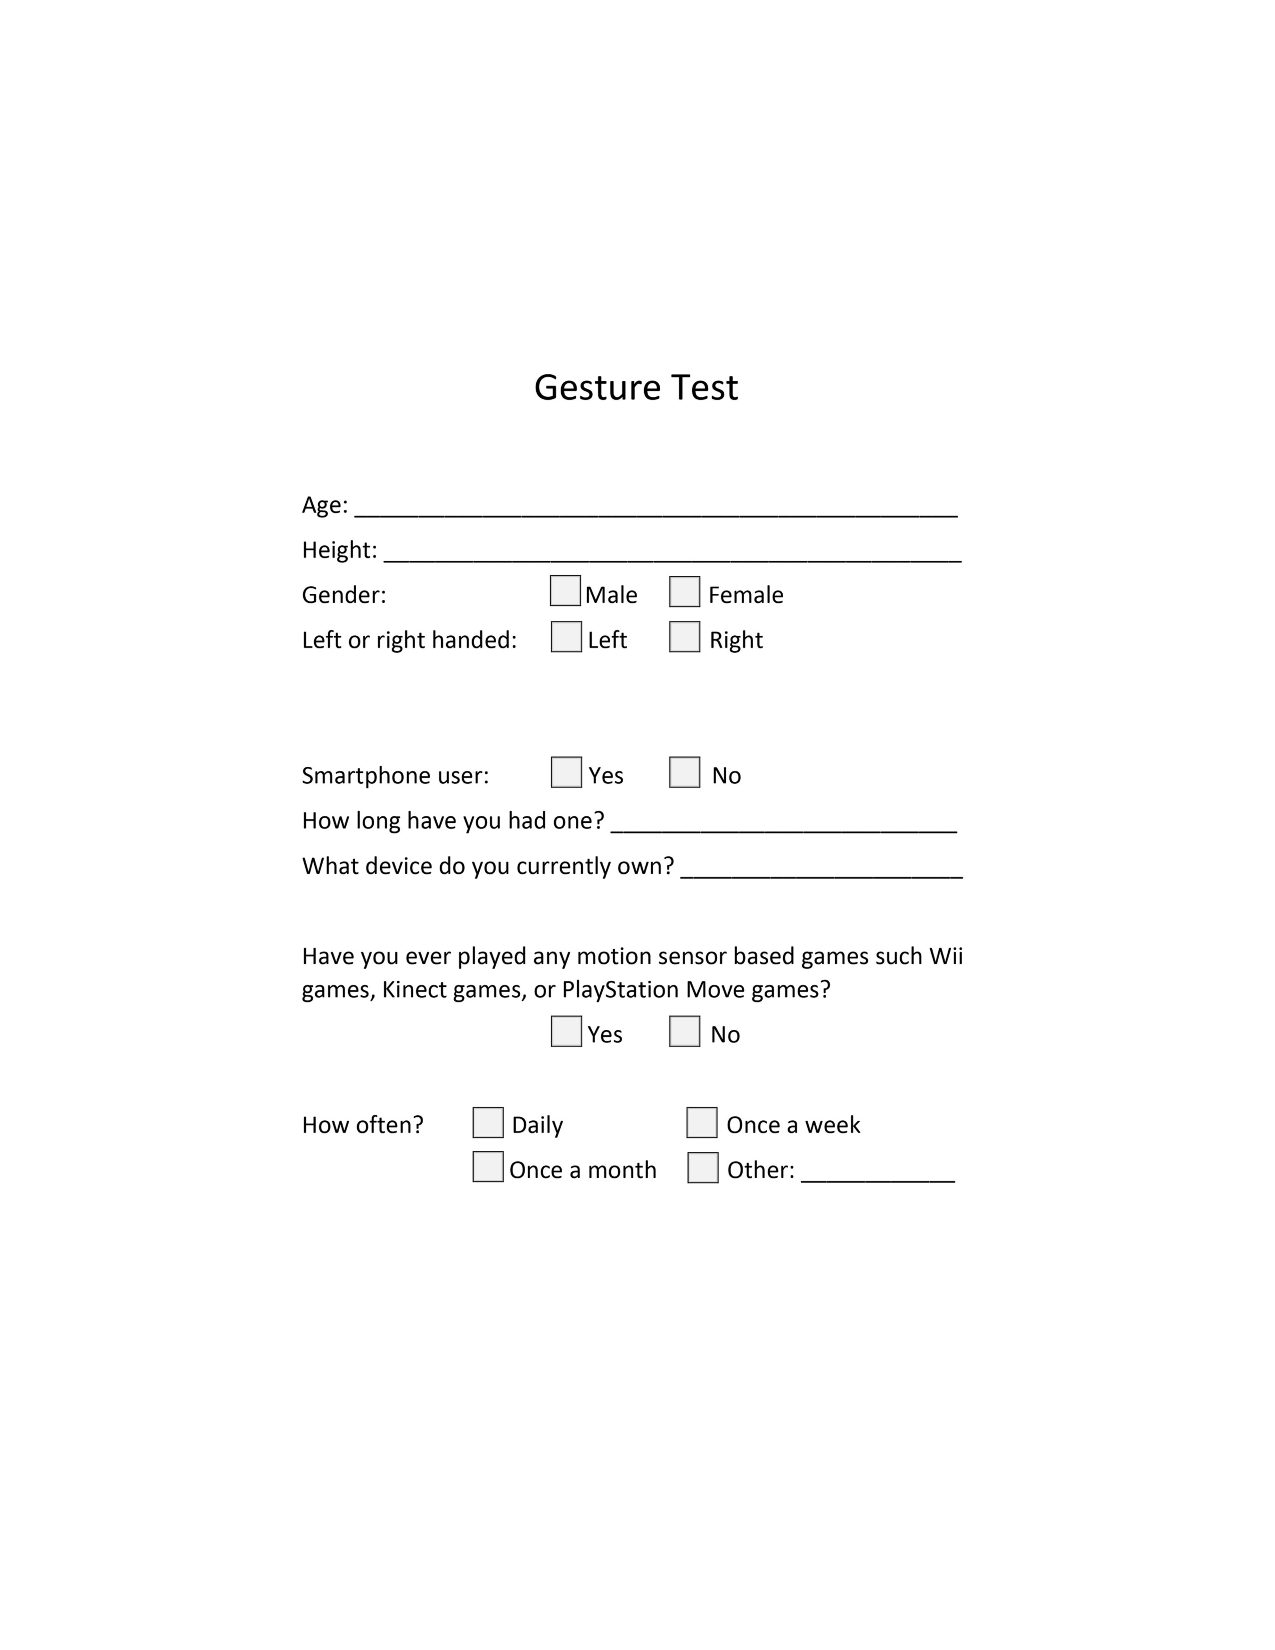
\includepdf[clip,trim=0cm 0cm 0cm -4cm,pages={1},pagecommand={\subsection*{\demographics}\addcontentsline{toc}{subsection}{\demographics}}]{docs/appendix/files/split_demo.pdf} 

\addbackpage
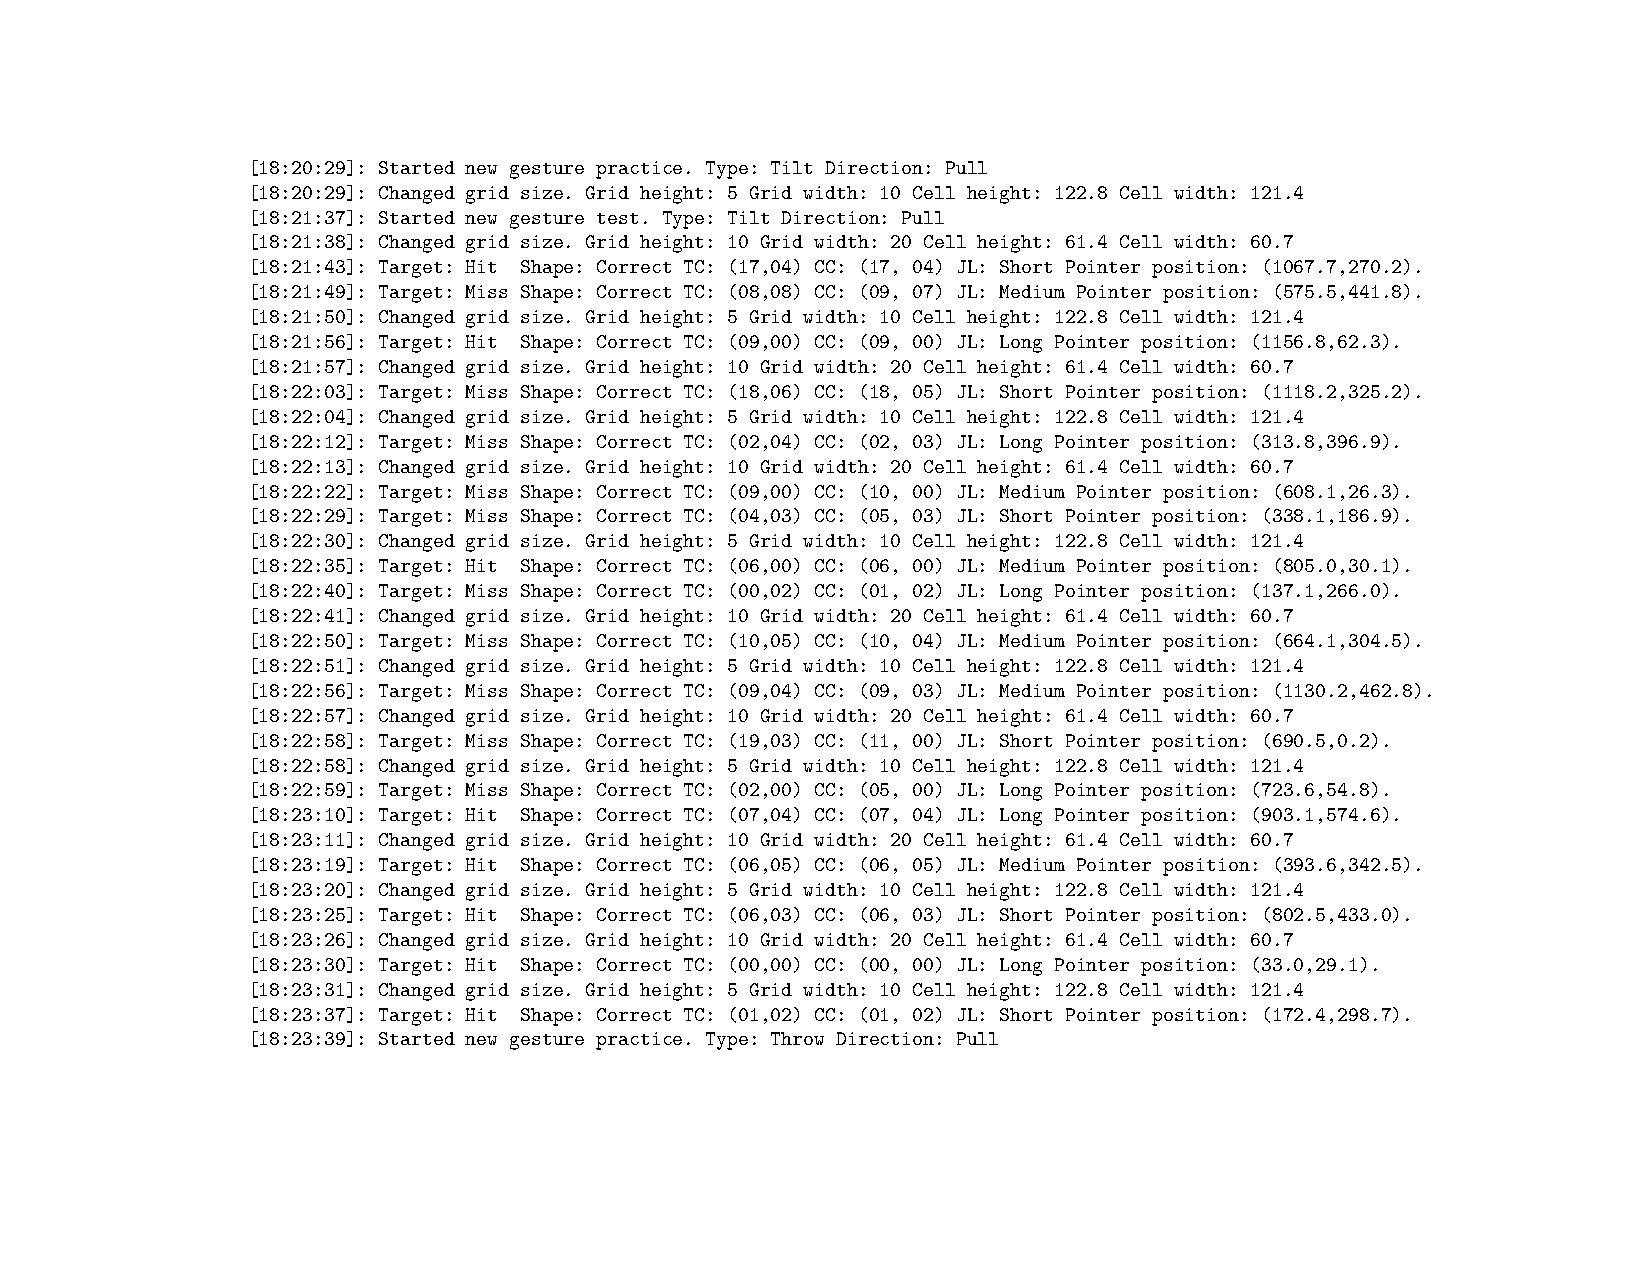
\includepdf[scale=0.95,landscape=true,clip,trim=0cm 0cm 0cm -2cm,pages={1},pagecommand={\subsection*{\rawtestlog}\addcontentsline{toc}{subsection}{\rawtestlog}}]{docs/appendix/files/testlog.pdf} 
\includepdf[scale=0.95,landscape=true,clip,trim=0cm 0cm 0cm 0cm,pages={2-last},pagecommand={}]{docs/appendix/files/testlog.pdf}
\subsection*{\rawcommentslog}
\addcontentsline{toc}{subsection}{\rawcommentslog}
\verbatiminput{files/rawcomments.txt}

\addbackpage
\includepdf[clip,trim=0cm 0cm 0cm -2cm,pages={1},pagecommand={\subsection*{\oldpaper}\addcontentsline{toc}{subsection}{\oldpaper}}]{docs/appendix/files/oldpaper.pdf} 
\includepdf[clip,trim=0cm 0cm 0cm 0cm,pages={2-last},pagecommand={}]{docs/appendix/files/oldpaper.pdf}
% Appendix input end
% Appendix end


\includepdf[pages=-,pagecommand={\thispagestyle{empty}}]{back.pdf} % The last page

\end{document}